\documentclass[a4paper,twoside]{memoir} 
\usepackage[utf8]{inputenc}
\usepackage[frenchb]{babel}
\usepackage[T1]{fontenc}

%
\usepackage{graphicx}
\usepackage{tikz}
\usepackage{float}
\usepackage{framed}




%\usepackage[final]{pdfpages} 

%
\usepackage{amsmath}



%%%%%%%%%style%%%%%%%
%Définition de l'en-tête des pages :

\copypagestyle{memoirStylePages}{headings}
\makerunningwidth{memoirStylePages}{\textwidth}
\makeheadrule{memoirStylePages}{\textwidth}{\normalrulethickness}
%\makefootrule{memoirStylePages}{\textwidth}{\normalrulethickness}{0pt}
\makeevenhead{memoirStylePages}{\itshape\leftmark}{}{}
\makeoddhead{memoirStylePages}{}{}{\itshape\leftmark}
\makeevenfoot{memoirStylePages}{}{\thepage}{}
\makeoddfoot{memoirStylePages}{}{\thepage}{}

%
%\makepsmarks{memoirStylePages}{%
%  \createmark{chapter}{left}{nonumber}{}{}
%}

\pagestyle{memoirStylePages}

\usepackage[
  a4paper,
  twoside,
  bindingoffset=1cm,
  inner=1cm,
  outer=1cm,
  top=3cm,
  bottom=3.5cm,
  headsep=1.2cm
]{geometry}

%\pagestyle{plain}

\pagenumbering{arabic}

%changement de la numérotation équation
\renewcommand{\theequation}{Eq. \thechapter.\arabic{equation}}

% interligne
\renewcommand{\baselinestretch}{1.5}

% Hyperlien
\usepackage{hyperref}
\hypersetup{
    colorlinks,
    citecolor=blue,
    filecolor=blue,
    linkcolor=blue,
    urlcolor=blue
}

%Définir les captions pour les figures :
\usepackage[font=it,labelfont=bf,labelsep=colon]{caption}

%Définir la profondeur des numérotations 
\setcounter{secnumdepth}{4}
\setcounter{tocdepth}{4}

%%%%%%%%end style%%%%%%%

 \def\pgfsys@svg@newline{^^J}

\begin{document}

%%%%%%%%%%%%%%
\title{Thèse brouillon}
\author{Aurélien TROTIER}
\date{\today}
\maketitle
%%%%%%%%%%%%%

%\chapter{Introduction}
\setlength{\footskip}{50pt}
\label{Chap1}

Durant les trente dernières d'années, le développement de méthodes permettant de modifier facilement le génotype ainsi que l'amélioration de la micro-chirurgie ont permis de mimer de nombreuses pathologies humaines chez l'animal ou bien d'en modifier la physiologie. Ces avancées ont joué un rôle important dans la recherche biomédicale qui a vu une forte augmentation de l'utilisation de modèles animaux, en particulier de souris et de rat. En effet, ceux-ci sont régulièrement utilisés pour leurs faibles coût d'entretien, leurs cycles de reproduction courts, leurs disponibilités et leurs relatives facilités de transport. En parallèle de ces avancées, de nombreuses méthodes permettant d'étudier ces modèles ont été découvertes, développées, perfectionnées ou adaptées à une utilisation sur le petit animal. Développer l'imagerie est crucial afin de pouvoir phenotyper et suivre ces modèles. 
\medbreak

Plusieurs modalités sont disponibles pour l'imagerie du petit animal comme la tomographie par émission de positons (TEP) ou monophotonique (TEMP), la tomodensitométrie à rayons X, l'imagerie optique, l'imagerie ultrasonore et l'imagerie par résonance magnétique (IRM). Chaque technique présente des avantages et des inconvénients que ce soit en terme de résolution spatiale, de résolution temporelle, de sensibilité, de spécificité, etc. De par leurs particularités inhérantes aux principes physiques, ces modalités sont donc complémentaires. Certaines seront à favoriser en fonction de l'application et du type d'information à recueillir.
\medbreak

Dans le cas de l'imagerie du système cardiovasculaire de la souris \textit{in vivo} plusieurs spécificités sont à noter. La modalité doit être la moins invasive possible, suffisamment sensible, offrir une résolution spatiale élevée et des contrastes élevés modulables et enfin plusieurs types d'informations doivent être recueillies :
\begin{enumerate}
 \item Des informations anatomiques sur la forme des vaisseaux, du cœur etc.
 \item Des informations fonctionnelles sur la contraction du coeur, la dilatation des artères ou bien les vitesses des flux.
\end{enumerate}
Seules l'imagerie par ultrasons et l'IRM peuvent répondre à ces besoins. Cependant l'IRM permet d'obtenir une visualisation en profondeur des tissus contrairement aux ultrasons dont la profondeur est limitée (de 5 à 15 mm) par la résolution spatiale que l'on souhaite obtenir. De plus, l'imagerie 3D disponible en IRM rend l'acquisition très peu opérateur-dépendant alors que la plupart des systèmes ultrasonores disponible ne permettent que des acquisitions 2D et donc des mesures peu reproductibles. L'IRM, malgré son coût élevé, apparaît donc comme un candidat idéal puisqu'elle répond à la plupart des exigences de l'imagerie du petit animal.

\medbreak
Le principe de l'IRM a vu le jour en 1973 dans une publication de Paul Lauterbur \cite{lauterbur1973image} après 30 ans de recherche sur la résonance magnétique nucléaire (RMN) qui consiste à mesurer le signal produit par un échantillon placé en présence d'un champ magnétique statique qui est ensuite excité par une onde de radiofréquence oscillant à la fréquence particulière de résonance du noyaux que l'on souhaite imager. Depuis, de nombreuses avancées techniques ont fait de l'IRM un outil indispensable dans le domaine de l'imagerie bio-médicale. Aujourd'hui, les imageurs par résonance magnétique utilisés en clinique ont généralement des champ statique de 1,5T ou 3T qui permettent d'obtenir de manière non invasive des images avec différents contrastes selon les paramètres utilisé. Ce très bon contraste permet d'obtenir une très bonne visualisation des structures anatomiques. La percée de l'IRM repose fortement sur sa capacité à obtenir des informations sur une large étendue d'autres paramètres allant de la densité de proton, de la diffusion, des vitesses de flux et de la température jusqu'à des paramètres plus complexes comme la distribution du sang, l'activité cérébrale ou bien l'orientation des faisceaux de fibres nerveuses.

\medbreak
D'un autre côté, l'IRM fait face à deux principales limitations qui sont accrues lors du passage de l'imagerie clinique à l'imagerie pré-clinique. La première est la faible sensibilité de cette modalité qui pose problème dans le cas de l'imagerie de la souris puisqu'il y a un rapport d'environ 1/3000 avec la masse de l'homme. Les résolutions à atteindre pour pouvoir observer les régions anatomiques sont donc bien plus importantes ($< 200 \mu m$ isotrope), ce qui génère une considérable diminution du rapport \gls{SSB} des images. Pour compenser cette diminution la tendance a été d'augmenter le champ statique des imageurs pré-cliniques afin d'accroître la polarisation. Ainsi, les imageurs pré-cliniques ont généralement des valeurs de champ statique supérieur à 4,7T. Cependant, cette augmentation provoque d'autres problèmes comme une diminution des valeurs $T_1$ des tissus, une modification des effets des agents de contraste, une baisse de l'homogénéité du champ magnétique et une augmentation du dépôt d'énergie lors de l'excitation radiofréquence. Une autre alternative pour compenser la faible sensibilité est l'accumulation du signal mais cette méthode allonge fortement les temps d'acquisition car l'augmentation du rapport \gls{SSB} est proportionnelle à la racine carré du nombre d'accumulation.
La deuxième différence importante entre l'humain et la souris est la fréquence des mouvements physiologiques que ce soit cardiaque ou respiratoire. Celle-ci est bien plus importante, par exemple, le rythme cardiaque d'une souris non anesthésiée est de 500 à 600 battements par minutes (bpm) contre 50 à 90 chez l'Homme. La résolution temporelle d'acquisition des images doit donc être augmentée pour permettre d'observer le cœur durant différentes phases du cycle cardiaque.

\medbreak
Pour ces deux principales raisons, l'IRM cardiovasculaire chez la souris est un véritable défi et il est nécessaire de développer des séquences d'acquisitions adaptées au petit animal que ce soit en terme de gain en rapport \gls{SSB}, de réduction du temps d'acquisition ou de sensibilité aux artefacts de mouvements. L'utilisation de séquence avec des trajectoires alternatives semble être une voie prometteuse et en particulier les trajectoires non cartésiennes qui permettent de progresser sur chacune de ces limitations. L'idée d'utiliser des trajectoires non-cartésienne d'échantillonnage du signal n'est pas nouvelle. Lauterbur utilisait déjà l'une d'entre elles dans son article de 1973 \cite{lauterbur1973image}, cependant cette méthode fut rapidement remplacée par les méthodes cartésiennes grâce à leur faible sensibilité aux erreurs instrumentales des premiers systèmes d'imagerie par résonance magnétique. Dans ces travaux de thèse c'est cette stratégie connue sous le nom d'imagerie radiale qui sera développée car elle présente des propriétés intéressantes par rapport à l'imagerie cartésienne qui viennent de la géométrie particulière de recueil des données.

\medbreak
L'objectif de cette thèse est de développer de nouvelles méthodes 3D d'imagerie cardio-vasculaire chez le petit animal basées sur des trajectoires radiales d'échantillonnage du signal. L'aspect 3D des séquences n'est pas anodin puisqu'il permet d'augmenter la résolution dans la direction de coupe, de gagner en rapport \gls{SSB} par rapport à des séquences à 2D. De plus, dans le cas de résolution pratiquement isotrope, le positionnement des coupes d'imagerie est facilité car il est possible de reconstruire des coupes a posteriori selon d'autres plans. Cependant les acquisitions 3D requièrent généralement un temps d'acquisition plus long. Une partie du travail dans cette thèse a consisté à réduire ces durées par rapport à celle que l'on peut trouver actuellement dans la littérature.

Dans cette optique, nous avons développé quatre méthodes d'IRM cardiovasculaire 4D (3D résolue dans le temps). 
Deux méthodes permettant d'obtenir des informations anatomiques et fonctionnelles et deux autres méthodes permettant de visualiser et de quantifier la vitesse des flux sanguins. 
\medbreak


Cette thèse est organisée de la manière suivante : Le chapitre 2 présente le principe de l'imagerie radiale et évoque ses propriétés principales ainsi que la reconstruction particulière de ce type d'acquisition. Le chapitre 3 présente l'amélioration d'une séquence développée au sein du laboratoire en 2006 permettant de visualiser l'avancée des flux sanguins. L'implémentation d'une méthode radiale de type projection-reconstruction couplée à une répartition des trajectoires selon une méthode doublement pseudo-aléatoire a permis de fortement réduire les temps d'acquisitions tout en augmentant la résolution spatiale. 
Les chapitres 4 à 6 présentent de nouvelles méthodes basées sur l'injection d'agent de contraste à base de nanoparticules de fer couplé à l'utilisation de séquences radiales à temps d'écho ultra-court. Cette combinaison permet de rehausser le signal du sang et d'obtenir un contraste positif entre le sang et le myocarde durant une période compatible avec le temps d'acquisition des séquences. Le chapitre 4 présente une séquence 4D (3D résolue dans le temps) anatomique synchronisée sur le rythme cardiaque grâce à des électrodes ECG. La stratégie développée permet de reconstruire, à partir d'un même jeu de donnée, des images avec une forte résolution spatiale et des images avec une forte résolution temporelle. Le chapitre 5 s'attarde sur une méthode d'imagerie anatomique 4D auto-synchronisée sur le rythme cardiaque permettant l'imagerie de modèle animaux dont les signaux électriques de conduction dans le coeur sont perturbés et qui limitent l'utilisation d'électrodes pour la synchronisation sur le rythme cardiaque. Dans le chapitre 6, une méthode de quantification de la vitesse des flux 4D est détaillée, basée sur un module d'encodage des vitesses selon les 3 directions de l'espace positionnée avant une lecture du signal radial. Cette utilisation de la trajectoire radiale permet de limiter les artéfacts de provoqué par les flux turbulents lors de la contraction du coeur.
Le chapitre 7 récapitulera les principales avancées de ce travail et donnera un aperçu sur les futurs travaux cliniques et précliniques.






\chapter{Imagerie radiale}
\setlength{\footskip}{50pt}
\label{Chap2}
\section{Description de l'espace de Fourier}

Une expérience de RMN élémentaire standard nous permet de mesurer un signal provenant d'un volume mais il est impossible d'assigner une position spatiale aux protons à partir de ce seul signal. Cependant, l'information spatiale peut être indirectement obtenue en répétant cette expérience élémentaire avec l'application supplémentaire de différentes combinaisons de gradients de champs magnétiques dans 2 ou 3 directions. Les signaux recueillis peuvent alors être stockés dans une matrice que l'on appelle espace de Fourier (ou espace-K) à partir de laquelle une opération mathématique (Transformée de Fourier) permettra d'obtenir une image. 
Généralement, la construction d'une image nécessite le recueil d'une série de signaux appelés acquisitions. Pour chaque acquisition, une impulsion radiofréquence (RF) engendre une nouvelle valeur d'aimantation transverse à l'origine du signal et qui est alors échantillonnée selon une trajectoire particulière de l'espace de Fourier (figure \ref{fig:Signal2Image}).


\begin{figure}[h]
\centering
\line(1,0){400} \\
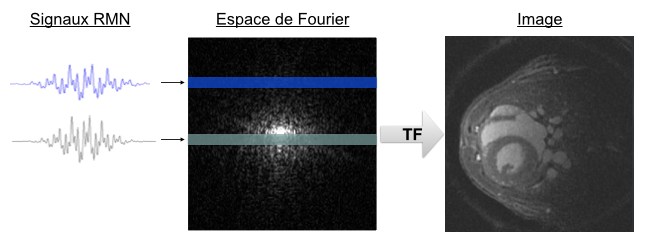
\includegraphics[scale=0.7]{./figure/chap2/Signal2Image.png}
\caption[Formation d'une image à partir de signal RMN]{\label{fig:Signal2Image} \textbf{Formation d'une image à partir du signal RMN.} Les signaux recueillis sont stockés dans l'espace de Fourier qui après une transformée de Fourier (TF) permet d'obtenir une image. }
\line(1,0){400} \\
\end{figure}

%V11 mars 2015. En principe, une image complète d'IRM peut être reconstruite à partir d'une seule acquisition en utilisant une trajectoire qui  parcoure tout l'espace de Fourier. C'est une méthode très souvent utilisé en imagerie fonctionnelle. Cependant, pour la plupart des applications cela entraine l'apparition d'artefacts dans l'image et d'une faible résolution spatial. Cela est due à la décroissance exponentielle du signal qui limite la fenêtre de temps d'acquisition exploitable. Mais cette fenêtre d'acquisition est aussi dicté par la performance du système de gradient et les contraintes physiologiques qui limite la vitesse à laquelle l'espace de Fourier peut être traversé. Il en résulte que la plupart des méthodes d'imagerie IRM utilisent de multiple acquisitions, chacune d'entre elles permettant de recueillir les informations d'une partie de l'espace de Fourier.

En principe, une image complète d'IRM peut être reconstruite à partir d'une seule acquisition en utilisant une trajectoire qui  parcourt tout l'espace de Fourier. Cependant, pour la plupart des applications cela entraîne l'apparition d'artefacts dans l'image et d'une faible résolution spatiale. Cela est dû à la décroissance exponentielle du signal qui limite la fenêtre de temps d'acquisition exploitable. Mais cette fenêtre d'acquisition est aussi dictée par la performance du système de gradient et les contraintes physiologiques qui limitent la vitesse à laquelle l'espace de Fourier peut être parcouru. Il en résulte que la plupart des méthodes d'imagerie IRM utilisent de multiples acquisitions, chacune d'entre elles permettant de recueillir les informations d'une partie de l'espace de Fourier.

Une partie du développement de nouvelles méthodes d'acquisition en IRM consiste à modifier la stratégie et les trajectoires permettant de remplir l'espace de Fourier.


\subsection{Parcours de l'espace de Fourier}
\label{subsec:Parcours}

Un déplacement dans l'espace de Fourier s'effectue grâce à l'application des gradients de codage de l'espace. L'application d'un gradient induit en effet une variation de la fréquence de précession des spins dépendante de leurs positions dans l'espace. Suite à l'arrêt des gradients, les spins précessent à nouveau à la même fréquence mais ont accumulé une différence de phase qui dépend de leur position par rapport à l'isocentre de l'imageur. Le signal mesuré provenant de l'ensemble des ces spins est stocké dans l'espace de Fourier aux coordonnées définies par l'équation :
\begin{equation}
\overrightarrow{k(T)}= \frac{\gamma}{2\pi} \int_0^T \overrightarrow{G(t)}dt
\end{equation}

Le déplacement entre deux points de l'espace de Fourier est proportionnel à l'aire de l'ensemble des gradients appliqués, plus l'aire est importante plus la distance parcouru entre deux points le sera aussi. En appliquant des gradients selon des axes différents, il est possible de parcourir l'espace de Fourier en 2D comme dans la figure \ref{fig:ParcoursKspace} ou en 3D avec l'ajout d'un axe de gradient supplémentaire.

\begin{figure}[H]
\centering
\line(1,0){400} \\
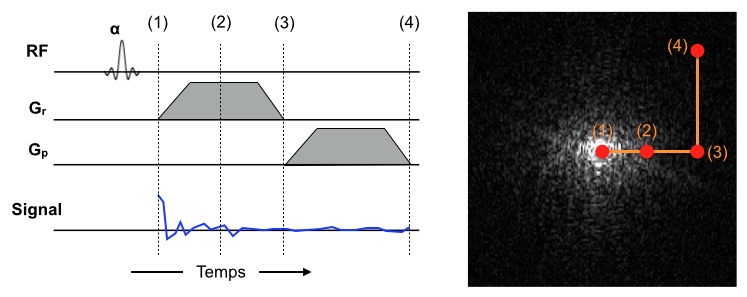
\includegraphics[scale=0.6]{./figure/chap2/ParcoursKspace.png}
\caption[Parcours de l'espace de Fourier en fonction de l'application de gradients.]{\label{fig:ParcoursKspace} \textbf{Parcours de l'espace de Fourier en fonction de l'application de gradients.} Après l'impulsion radiofréquence d'angle $\alpha$, l'espace de Fourier est parcouru suivant un axe horizontal grâce au gradient appliqué sur l'axe $G_r$ puis selon un axe vertical grâce à l'application d'un gradient sur l'axe $G_p$. Les positions des points 1 à 4 dans l'espace de Fourier sont indiqués sur le chronogramme.}
\line(1,0){400} \\
\end{figure}


\subsection{Propriété de l'espace de Fourier}

L'espace de Fourier, de par sa nature, dispose de nombreuses propriétés qui peuvent être exploitées lors du développement de nouvelles méthodes d'acquisition. 

\subsubsection{Régions centrales et extérieures}
\label{subsec:KSpaceRegion}
Les régions centrale et périphérique de l'espace de Fourier contribuent différemment à la construction de l'image. La figure \ref{fig:kSpaceResSig} illustre le fait que le centre de l'espace contient les basses fréquences de l'image et renseignent principalement sur le signal et le contraste, alors que la périphérie encodant les hautes fréquences spatiales renseignent quant à eux sur les détails, les contours ainsi que le bruit.

\begin{figure}[H]
\centering
\line(1,0){400} \\
\includegraphics[scale=0.7]{./figure/chap2/kSpaceResSig.png}
\caption[Contribution des données de l'espace de Fourier en fonction de leur position.]{\label{fig:kSpaceResSig} \textbf{Contribution des données de l'espace de Fourier en fonction de leur position.} Les régions centrale et/ou périphérique de l'espace de Fourier sont utilisées pour reconstruire les images grâce à une transformée de Fourier. La reconstruction avec le centre de l'espace donne une image floue mais contrastée alors que la périphérie de l'espace donne une image détaillée mais avec peu de signal et de contraste.}
\line(1,0){400} \\
\end{figure}

\subsubsection{Résolution et champ de vue}

La résolution de l'image est donnée par la taille de l'espace de Fourier qui est échantillonnée; plus celle-ci est grande plus l'image sera résolue.
\begin{equation}
\Delta x = \frac{1}{2*k_{max}}
\end{equation}
où $k_{max}$ est la position du point échantillonné la plus éloignée du centre de l'espace de Fourier. Le champ de vue est quant à lui déterminé par la densité d'échantillonnage de cette région. Pour obtenir un grand champ de vue, notée ici FOV (Field of view), il faut échantillonner de manière dense l'espace de Fourier. Le FOV est relié à la distance d'échantillonage $\delta k$ par la relation suivante :
\begin{equation}
\label{eq:FOV}
FOV = \frac{1}{\Delta k}
\end{equation}
Généralement, l'espace de Fourier est échantillonné de manière à respecter le critère de Nyquist selon lequel la fréquence d'échantillonnage (1/$\delta t$) doit être au moins 2 fois supérieure à la plus haute fréquence contenue dans le signal. Ce critère aboutit à la relation :
\begin{equation}
\Delta k =\frac{2k_{max}}{n} \leq \frac{1}{FOV}
\end{equation}
où $n$ correspond au nombre de points échantillonnés pour une acquisition. Une violation du critère de Nyquist créera des artefacts dans l'image dépendant du type de trajectoire utilisé pour échantillonner l'espace de Fourier (figure \ref{fig:Undersamp}).
\begin{figure}[H]
\centering
\line(1,0){400} \\
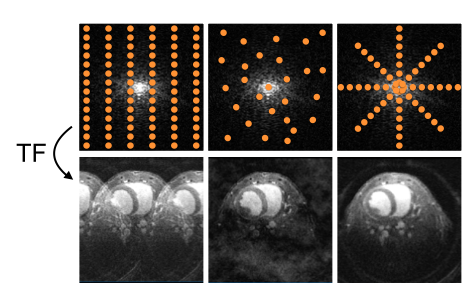
\includegraphics[scale=1]{./figure/chap2/Undersamp.png}
\caption[Sous-échantillonnage de l'espace de Fourier.]{\label{fig:Undersamp} \textbf{Sous-échantillonnage de l'espace de Fourier.} La violation du critère de Nyquist introduit des artefacts dans le domaine image qui dépendent de la trajectoire utilisée. A gauche : Avec une fréquence d'échantillonnage insuffisante d'un facteur 2 pour une acquisition cartésienne, on observe des artefacts de repliement. Au milieu : avec un espace sous-échantillonné aléatoirement avec un facteur 2, on observe des artefacts incohérents. A droite : avec un espace sous-échantillonné 5 fois avec des trajectoires radiales, on observe une diminution de la résolution.}
\line(1,0){400} \\
\end{figure}

\subsection{Trajectoire d'échantillonnage}

La trajectoire la plus couramment utilisée est la trajectoire cartésienne qui consiste en l'acquisition de lignes parallèles de l'espace de Fourier (figure \ref{fig:TrajCart}). Cela s'explique par sa reconstruction extrêmement simple, rapide et robuste qui utilise la Transformée de Fourier Rapide (noté FFT pour "Fast Fourier Transform"), un algorithme de calcul de la transformée de Fourier discrète appellé, selon chaque axe. Et surtout, la reconstruction à partir de cette trajectoire est peu sensible à de nombreuses sources d'imperfections. Le principal problème de ce schéma d'acquisition est sa sensibilité au mouvement et ses artefacts cohérents de repliement qui sont créés en cas de sous-échantillonnage.
%%%%%Modif 08/03/2015
%Cependant, la conception d'une trajectoire est relativement libre et peut permettre d'obtenir certaines propriétés intéressante que ce soit en terme de temps, d'acquisition, faible sensibilité aux mouvement ou pour des applications spécifiques. 
Bien que ces schémas de trajectoires soient majoritairement employés, de nombreux autres ont été développés et sont décrits dans la littérature. Parmis ceux-ci, les trajectoires radiales ont des propriétés intéressantes pour des applications sur le petit animal.

\begin{figure}[h]
\centering
\line(1,0){400} \\
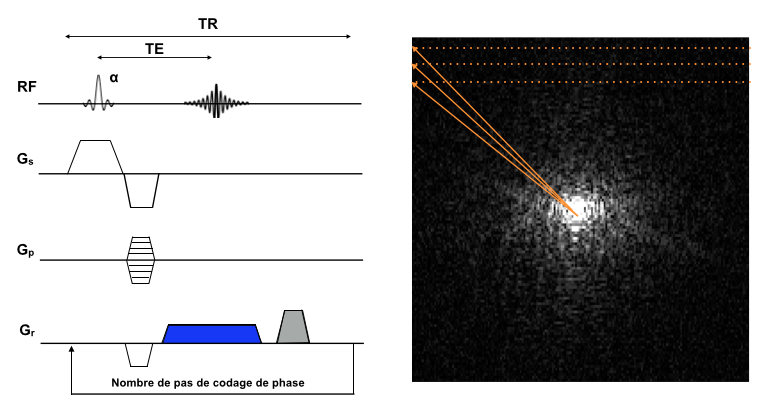
\includegraphics[scale=0.5]{./figure/chap2/TrajCart.png}
\caption[Chronogramme d'une séquence cartésienne]{\label{fig:TrajCart} \textbf{Chronogramme d'une séquence cartésienne}. Pour les trajectoires cartésiennes, la lecture du signal s'effectue durant l'application d'un gradient de lecture constant (selon $G_r$). Les autres gradients servant à positionner le premier point de la lecture après l'impulsion radiofréquence basculant l'aimantation dans le plan transverse.}
\line(1,0){400} \\
\end{figure}

\section{Trajectoire radiale dans l'espace de Fourier}

\subsection{Principe}
Le schéma d'acquisition radiale a tout d'abord été proposé par Lauterbur en 1973 \cite{lauterbur1973image}. Peu après l'introduction des scanners commerciaux, les trajectoires radiales ont été remplacées par des trajectoires cartésiennes car celles-ci étaient plus robustes aux hétérogénéités de champs $B_0$ et à la non-linéarité des gradients qui étaient très présents sur les premiers scanners IRM. Au fil des années, un regain d'intérêt est apparu pour les séquences radiales grâce aux progrès techniques en particulier sur la compensation des courants de Foucault dans les gradients et la meilleure homogénéité du champ statique. 

En imagerie radiale, le signal IRM est échantillonné selon des trajectoires suivant les rayons ou les diamètres d'un disque qui permettent d'obtenir respectivement une séquence à temps d'écho ultra-court (UTE) ou une séquence projection-reconstruction (PR). Dans le cas d'une séquence 2D la trajectoire est inscrite dans un disque et, pour les séquence 3D, dans une sphère. Les différentes trajectoires sont illustrées sur la figure \ref{fig:TrajRad}.

\begin{figure}[H]
\centering
\line(1,0){400} \\
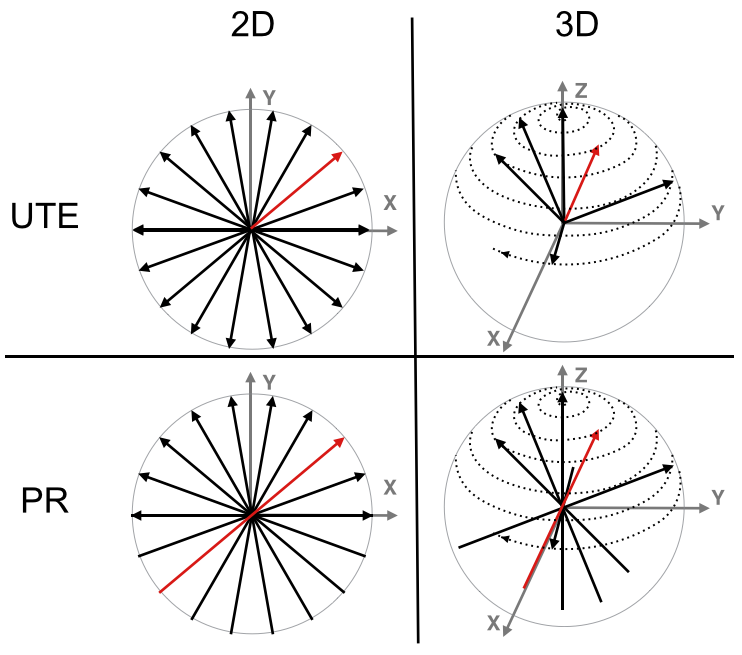
\includegraphics[scale=0.5]{./figure/chap2/TrajRad.png}
\caption[Représentation des types de trajectoires radiales.]{\label{fig:TrajRad} \textbf{Représentation des types de trajectoires radiales.} Les trajectoire radiale 2D et 3D sont représentées schématiquement dans le cas d'une acquisition UTE ou PR.}
\line(1,0){400} \\
\end{figure}




\subsection{Description mathématique}

Pour recueillir le signal selon les trajectoires radiales, l'amplitude des gradients varies selon les 3 axes simultanément selon l'équation :
\begin{equation}
\label{eq:AngleRadial}
\begin{split}
	G_x & =G\cos(\phi)\sin(\theta)\\
	G_y & =G\sin(\phi)\sin(\theta)\\	
	G_z & =G\cos(\theta)
\end{split}
\end{equation}
où $\theta$ et $\phi$ correspondent aux angles définis dans la figure \ref{fig:SphereCoord}.
Puisque les gradients dans les 3 directions sont utilisés pour chaque acquisition radiale de l'espace de Fourier, ils sont considérés comme des gradients de lecture plutôt que des gradients d'encodage de fréquence et de phase comme pour une acquisition cartésienne. Dans le cas d'une acquisition 2D, seul l'angle $\theta = \frac{\pi}{2}$ est utilisé ce qui a pour conséquence de fixer la valeur du gradient z à 0 et de ne faire varier les gradients que selon les axes x et y en fonction des valeurs de $\phi$.

\begin{figure} [H]
\centering
\line(1,0){400} \\
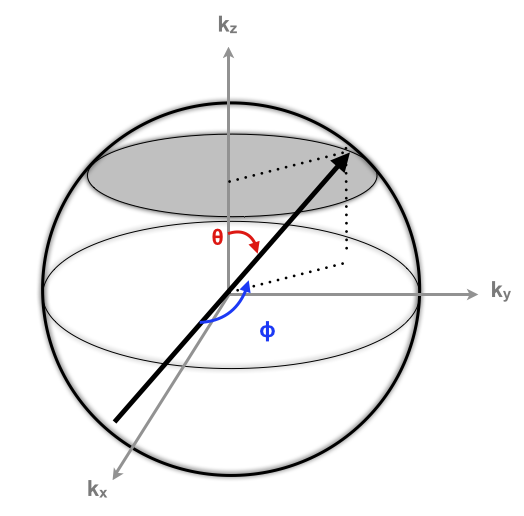
\includegraphics[scale=0.5]{./figure/chap2/SphereCoord.png}
\caption[Définition des coordonnées sphériques.]{\label{fig:SphereCoord} \textbf{Définition des coordonnées sphériques.} Représentation des angles $\theta$ et $\Phi$ utilisés  pour définir les trajectoires radiale en 3 dimensions.}
\line(1,0){400} \\
\end{figure}

Comme pour le cas cartésien, la distance entre deux points échantillonnés sur une projection est généralement définie par la taille du FOV désiré grâce à l'équation \ref{eq:FOV} et n, le nombre de points échantillonnés est définies par la résolution de base désirée. Avec une trajectoire radiale, ces deux paramètres ne sont pas suffisants pour définir la résolution spatiale réelle de l'image car celle-ci dépend aussi de $n_p$, le nombre de projections utilisé. Pour satisfaire le critère de Nyquist, d'après la littérature \cite{bernstein2004handbook}, il est nécessaire d'utiliser un nombre de projections égal à :
\begin{equation}
\label{eq:NyquistRad}
\begin{aligned}
	(2D)\;\;\;\; n_p = \frac{\pi}{2} \times n \\
	(3D)\;\ \ n_p = \pi \times n^2 
\end{aligned}
\end{equation}
qui assure que la distance entre deux points de projections voisines soit inférieure ou égale à $\Delta k$.

\subsection{Chronogramme des séquences}

Comme décrit dans la partie \ref{subsec:Parcours}, une trajectoire dans l'espace de Fourier correspond à l'application de gradient avec une intensité donnée selon un ordre chronologique. Pour représenter une séquence, il est courant d'utiliser un chronogramme qui présente entre autre les gradients de lecture, de phase et de sélection de coupe que l'on notera respectivement $G_r$,$G_p$ et $G_s$ ainsi que les impulsions RF. Les chronogrammes de la séquence radiale 3D PR et UTE sont présentés dans la figure \ref{fig:KspacePR}.

\begin{figure}[h]
\centering
\line(1,0){400} \\
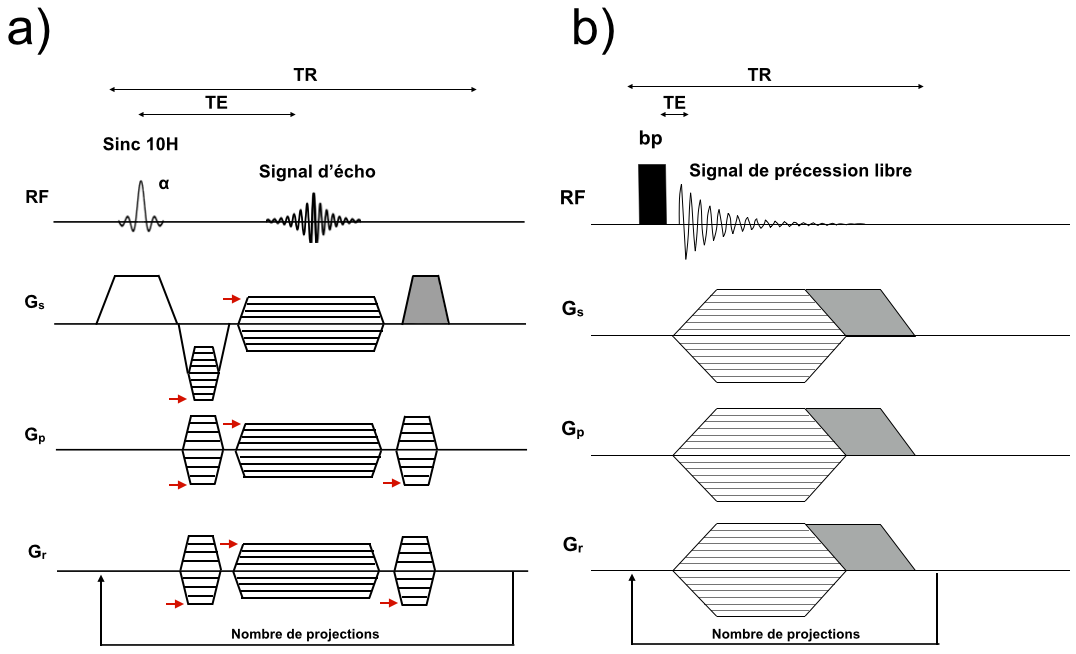
\includegraphics[scale=0.4]{./figure/chap2/KspacePR.png}
\caption[Chronogramme des séquences radiales.]{\label{fig:KspacePR} \textbf{Chronogramme des séquences radiales.} (a) chronogramme d'une séquence radiale 3D PR. (b) Chronogramme d'une séquence radiale 3D UTE. Les gradients grisés permettent de déphaser l'aimantation résiduelle avant la prochaine excitation radiofréquence.} 
\line(1,0){400} \\
\end{figure}

La séquence PR débute avec une impulsion RF qui peut être sélective grâce à l'application d'un  gradient (suivant l'axe $G_s$) suivi par un gradient de rephasage qui compense l'évolution de phase indésirable causée par le gradient de sélection de coupe durant la seconde moitié de l'impulsion RF. Pour réduire la durée entre l'impulsion RF et la lecture du signal, les gradients de codage de l'espace sont appliqués en même temps que le gradient de rephasage de coupe pour atteindre une position périphérique de l'espace de Fourier. A partir de cette position, les gradients sont commutés avec une amplitude opposée de manière à parcourir diamétralement l'espace de Fourier. Durant ce déplacement, le signal est recueilli avec une fréquence d'échantillonnage fixe. La dernière étape de cette séquence consiste à déphaser l'aimantation résiduelle avec des gradients de déphasage de type "spoiler". Pour chaque répétition, l'amplitude des gradients de déphasage puis de "lecture" sont modulés par l'équation \ref{eq:AngleRadial} pour définir les différentes trajectoires des projections.

La séquence UTE est similaire à la séquence PR à ceci près qu'elle n'emploie pas 
de gradient de sélection/rephasage de coupe. La lecture s'effectuant à partir du centre, le signal recueilli est un signal de précession libre et non pas un signal d'écho.

Un autre type de séquence 3D radiale est très souvent utilisé, et appelé Stack-Of-Stars (Empilement d'étoiles). Cette séquence consiste en un empilement de plan contenant des trajectoires 2D UTE ou 2D PR. Le chronogramme de la séquence d'empilement UTE et la trajectoire correspondantes dans l'espace de Fourier sont présentés dans la figure \ref{fig:KspaceStackOfUTE}

\begin{figure}[H]
\centering
\line(1,0){400} \\
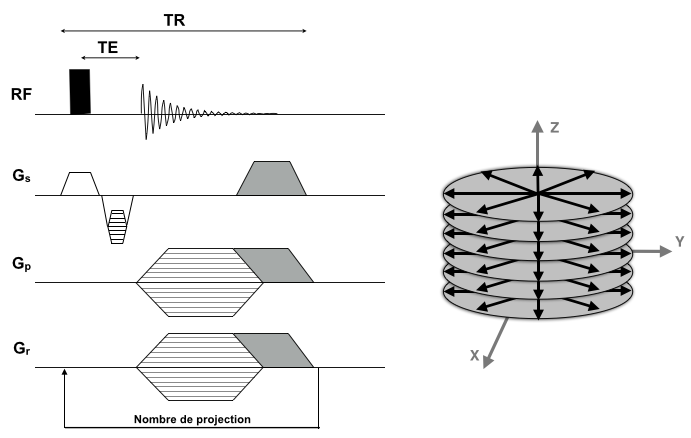
\includegraphics[scale=0.6]{./figure/chap2/KspaceStackOfUTE.png}
\caption[Chronogramme et trajectoire d'une séquence Stack-Of-Stars UTE.]{\label{fig:KspaceStackOfUTE} \textbf{Chronogramme et trajectoire d'une séquence Stack-Of-Stars UTE.} (a) Chronogramme d'une séquence radiale Stack-Of-Stars UTE. (b) Trajectoire d'une séquence Stack-Of-Stars UTE dans l'espace de Fourier. } 
\line(1,0){400} \\
\end{figure}

\subsection{Reconstruction}

\label{subsec:reconstruction}
Différentes approches sont utilisées pour la reconstruction des acquisitions radiales : la rétro-projection filtrée, le remaillage (gridding) ou la FFT non uniforme (nuFFT). Dans cette partie, c'est la reconstruction par remaillage qui sera détaillé puisque c'est cette dernière qui est la plus communément utilisée et qui a été appliquée pour ces travaux de thèse.

La méthode de reconstruction par remaillage a été introduite en imagerie médicale par O'Sullivan en 1985 \cite{o1985fast} et fut plus tard appliquée à la reconstruction d'images IRM recueillies avec des trajectoires d'acquisitions non-cartésiennes. Cette technique consiste à interpoler les points échantillonnés sur une grille rectilinéaire avant d'effectuer une reconstruction avec l'algorithme de FFT (figure \ref{fig:Gridding}).

\begin{figure}[h]
\centering
\line(1,0){400} \\
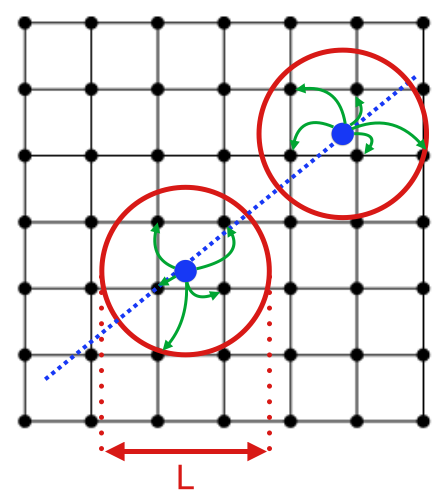
\includegraphics[scale=0.6]{./figure/chap2/Gridding.png}
\caption[Interprétation graphique de l'opération de remaillage.]{\label{fig:Gridding} \textbf{Interprétation graphique de l'opération de remaillage.} L'opération de gridding consiste à regarder quels points de la grille cartésienne (en noir) sont contenus autour d'un point échantillonné (en bleu) à une distance inférieure à $\frac{L}{2}$. La distance séparant chacun des points de la grille au point échantillonné est utilisée comme paramètre $d$ dans le kernel.} 
\line(1,0){400} \\
\end{figure}

Dans le cas de l'imagerie radiale, la densité de points variable dans l'espace de Fourier nécessite d'être compensée a priori ou a posteriori de l'interpolation. Généralement, la fonction de compensation en densité est utilisée comme un poids attribué à chaque point de l'espace de Fourier échantillonné. Pour disposer les points sur une grille cartésienne, le signal mesuré est convolué avec un kernel d'interpolation. La littérature a montré que l'utilisation d'un kernel Kaiser-Bessel est optimale pour l'opération d'interpolation des données pour les acquisitions radiales. Celui-ci permet d'optenir des images de bonnes qualité avec une taille du kernel $L$ raisonnable et est défini par :
\begin{equation}
  K_{kb}(d) = \left\{
      \begin{aligned}
         \frac{1}{L}I_0(\beta \sqrt{1-(2d/L)^2}) \;\;\;\;\;\;  |d| \leq \frac{L}{2}\\
	     0 \;\;\;\;\;\; |d| \leq \frac{L}{2}
      \end{aligned}
    \right.
\end{equation}
où $L$ correspond à la taille du kernel, d à la distance séparant le point à remailler d'un point de grille, $\beta$ est un facteur de forme et $I_0$ correspond à la fonction de bessel modifiée de première d'espèce d'ordre 0 et $I_0$ correspond à la fonction de bessel modifiée de première d'espèce d'ordre 0.
La taille du kernel $L$ impacte la qualité des images reconstruites, plus grand est sa taille plus l'image sera de bonne qualité. Cependant cela influera fortement sur le temps de reconstruction, potentiellement pour un gain faible en qualité. une valeur de 2 à 4 est généralement utilisée permettant d'obtenir une image avec une bonne qualité tout en limitant le temps de reconstruction. Le facteur $\beta$ est sélectionné en accord avec l'équation décrite par Beatty et al. \cite{Beatty:2005fk}. La forme du kernel est représentée dans la figure \ref{fig:KaiserBessel}.
\begin{figure}[H]
\centering
\line(1,0){400} \\
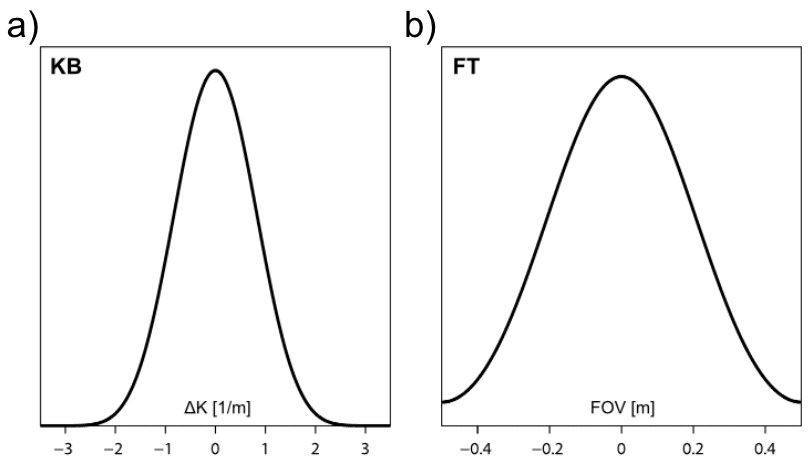
\includegraphics[scale=0.6]{./figure/chap2/KaiserBessel.png}
\caption[Représentation du filtre kernel Kaiser-Bessel.]{\label{fig:KaiserBessel} \textbf{Représentation du filtre kernel Kaiser-Bessel.} (a) Représentation dans le domaine de l'espace de Fourier du filtre kernel Kaiser-Bessel pour une valeur de $L = 6$ et $\beta = 13,8551$, où le champ de vue est normalisé à 1 m. (b) représentationdu kernel présentée en a) dans le domaine image par une transformée de Fourier .}
\line(1,0){400} \\
\end{figure}

Malheureusement la convolution avec un kernel d'une taille finie entraîne sur l'image obtenue après FFT des artefacts de modulation appelés effets roll-off (figure \ref{fig:deapod}). Cette modulation d'intensité de signal peut être compensée en divisant l'image par la transformée de Fourier du kernel qui est approximée par l'équation :
\begin{equation}
	FFT[K_{KB}](d) = \frac{\sin(\sqrt{(\pi L d)^2-\beta^2})}{\sqrt{(\pi L d)^2-\beta^2}}
\end{equation}
La convolution avec un kernel fini a aussi pour effet de créer des lobes secondaires qui sont repliés sur l'image.  Bien que l'amplitude initiale de ces lobes soit généralement faible avec un choix de kernel approprié, leurs intensités sont amplifiées par la correction de l'effet roll-off. Une solution simple à ce problème consiste à augmenter le champ de vue en effectuant le gridding sur une matrice plus grande, généralement d'un facteur 2. L'augmentation du champ de vue est ensuite corrigée en utilisant seulement les pixels centraux de l'image correspondant au champ de vue utilisé.

\begin{figure}[H]
\centering
\line(1,0){400} \\
\includegraphics[scale=0.6]{./figure/chap2/deapod.png}
\caption[ Correction de l'effet Roll-Off.]{\label{fig:deapod}\textbf{ Correction de l'effet Roll-Off.} Effet de la correction de l'effet Roll-Off sur un fantôme. La variation de signal entre le centre et les bords du fantôme est compensée par la division avec la transformée de Fourier du kernel utilisé pour le remaillage. Figure extraite d'une présentation de Otazo R. \cite{otazo:2014Reconstructi} .}
\line(1,0){400} \\
\end{figure}

La procédure de remaillage se compose donc des étapes suivantes :
\begin{enumerate}
\item Compensation en densité
\item Interpolation sur une grille par convolution avec un kernel
\item FFT
\item Correction de l'effet roll-off
\item Découpe de l'image
\end{enumerate}

\subsection{Avantages et désavantages de la trajectoire radiale}

La trajectoire radiale offre des propriétés uniques du fait de sa géométrie ou de l'ordonnancement de l'acquisition de l'espace de Fourier. Certaines de ces propriétés sont avantageuses par rapport à une acquisition cartésienne mais d'autres peuvent se transformer en inconvénients. Dans cette section, nous discuterons de ces propriétés en gardant en vue les applications possibles.
 
\subsubsection{Fonction d'étalement du point}

Pour comprendre les caractéristiques de n'importe quel système d'imagerie, il est souvent très intéressant d'étudier la fonction d'étalement du point (Point Spread Function : PSF). La PSF décrit la réponse du système à une impulsion (un dirac) et permet de conclure sur comment un objet est imagé par celui-ci. En IRM, la PSF est fortement liée à la trajectoire utilisée dans l'espace de Fourier. En ignorant les phénomènes de relaxation pour plus de simplicité, la PSF d'une séquence IRM peut être obtenue en reconstruisant une image avec des données égales à 1 suivant la trajectoire radiale.

La figure \ref{fig:PSF} présente : 1) les PSFs obtenues en fonction de $n_p$ le nombre de projection en imagerie UTE et 2) les images correspondantes acquises sur un thorax de souris avec une résolution de base de $n = 128$ pixels. D'après l'équation \ref{eq:NyquistRad}, pour la résolution de 128 pixels, il est nécessaire pour une acquisition UTE de recueillir 402 projections. Dans ce cas, on observe un pic au centre de la PSF bien distinct qui est entouré par des oscillations circulaires mineures dont les amplitudes diminuent en s'écartant du centre. Ces oscillations sont dues à l'utilisation d'un espace de Fourier fini, et sont à l'origine d'un effet dit de troncature. Si l'on diminue le nombre de projections $n_p$ utilisé pour la reconstruction, par exemple à 134 projections, on peut voir qu'une démarcation apparaît dans la PSF correspondante à une certaine distance du centre délimitant ainsi une région sans artefact (double flèches blanches) \cite{Scheffler:1998fk} et que des artefacts de "streaking" apparaissent en dehors de ce disque. De plus, la largeur à mi-hauteur du pic central est plus large ce qui traduit une légère diminution de la résolution. Chaque "point" de l'objet étant convolué avec la PSF durant la reconstruction, le motif de "streaking" apparaît sur l'image reconstruite à une distance correspondant à la taille de cette région sans artefact dans la PSF. Lorsque l'on réduit le nombre de projections utilisé, le diamètre de cette région diminue et les artefacts sont plus prononcés. Cela est particulièrement visible sur la PSF et l'image reconstruite avec 40 projections.
En 3D, les artefacts de "streaking" sont plus diffus ce qui se traduit plutôt comme un bruit sur l'image et permet donc un sous-échantillonnage plus important de l'espace \cite{Gu:2005aa}.

\begin{figure}[h]
\centering
\line(1,0){400} \\
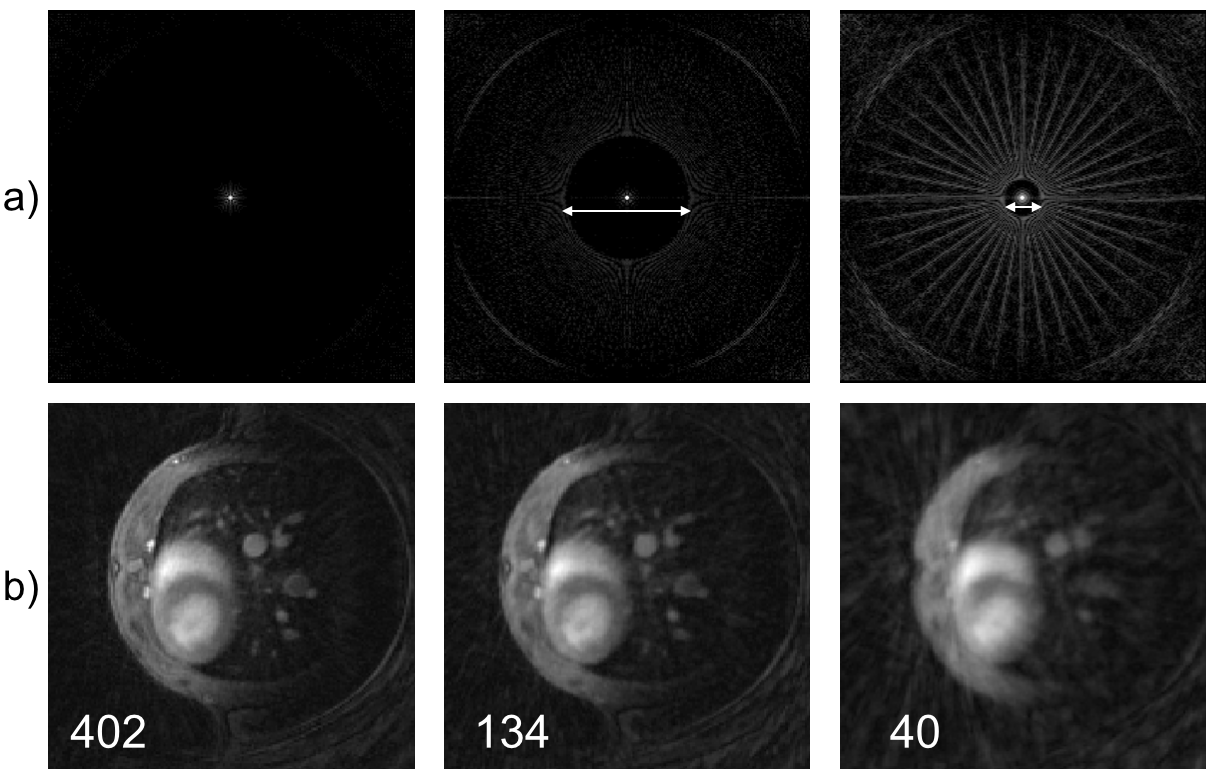
\includegraphics[scale=0.4]{./figure/chap2/PSF.png}
\caption[Effet du sous-échantillonnage sur la fonction d'étalement du point.]{\label{fig:PSF} \textbf{Effet du sous-échantillonnage sur la fonction d'étalement du point.} a) Images des PSFs reconstruitent à partir d'une trajectoire UTE 2D avec 402, 134 et 40 projections (résolution de base : 128 pixels) ainsi que (b) la reconstruction des images correspondantes acquises sur un thorax de souris. Les flèches blanches montrent le diamètre correspondant au champ de vue sans artefacts.}
\line(1,0){400} \\
\end{figure}

Par rapport à une trajectoire cartésienne, le nombre de lignes de l'espace de Fourier à recueillir est supérieur pour respecter le critère de Nyquist, ce qui augmente a priori le temps d'acquisition requis pour les séquences radiales. En pratique, il est néanmoins tout à fait possible de recueillir un nombre plus restreint de projection. Cela vient du fait que la région d'intérêt est souvent positionnée à l'intérieur de l'objet et donc que la présence d'artefacts de "streaking" aux bords de l'image peut ne pas gêner l'interprétation ou la quantification. Puisque la région centrale de la PSF est faiblement affectée par le nombre de projection utilisé, la trajectoire radiale offre une intéressante possibilité de sous-échantillonnage de l'espace de Fourier. Contrairement à l'acquisition cartésienne où une réduction du nombre de ligne recueillies aura pour conséquence une importante perte en résolution ou l'apparition d'artefact de repliement rendant l'image inutile, avec une trajectoire radiale, la plupart des informations restent visibles malgré la nette présence d'artefact de "streaking".

\subsubsection{Distribution des points échantillonnés}

En imagerie radiale, puisque toutes les projections passent par le centre du plan de Fourier, le nombre de points échantillonnés est plus important pour les basses fréquences de l'espace de Fourier que pour les hautes fréquences. Cela est très différent des acquisitions cartésiennes où toutes les fréquences sont couvertes de la même façon. Bien que le fait d'avoir une distribution variable de points échantillonnés dans l'espace de Fourier implique quelques difficultés pour la reconstruction (voir section \ref{subsec:reconstruction}), cela peut néanmoins devenir avantageux pour la plupart des objets à imager. En effet, la plupart des images du monde réel sont caractérisées par une concentration en énergie près du centre de l'espace de Fourier, cela est aussi bien valable pour les images médicales de tomographie que pour les autres images naturelles \cite{srivastava2003advances}. C'est pourquoi il est intéressant de mesurer les basses fréquences plus "précisément" même au détriment du nombre de points échantillonnés dans les régions périphériques de l'espace de Fourier contenant moins d'informations. 

Des images avec une faible résolution peuvent être reconstruites à partir d'une partie des projections recueillies. Cela est possible car le nombre de points échantillonnés est suffisamment dense au centre de l'espace de Fourier pour satisfaire le critère de Nyquist et obtenir une image sans artefact comme expliqué dans la section précédente. De nombreuses applications peuvent alors être envisagées, par exemple en 2D, une série d'images résolues dans le temps peuvent être extraites d'un jeu de donnée complet pour identifier et corriger des artefacts de mouvement qui peuvent survenir durant l'acquisition.

Une caractéristique supplémentaire de la géométrie radiale est que chaque projection apporte autant d'information sur les basses et hautes fréquences, alors qu'avec une acquisition cartésienne, les informations de basses fréquences ne sont contenues que dans quelques lignes. Cela fait de l'imagerie radiale une option attractive quand une mise à jour continue de l'image est importante, par exemple en imagerie interventionnelle (\cite{Peters:2004aa} ou bien pour de la prise de contraste dynamique \cite{Prieto:2010oq}). Récemment, une méthode alternative nommée "Highly Constrained Backprojection" utilise ce rafraîchissement constant de l'image durant l'injection d'un agent de contraste. Cette méthode autorise des sous-échantillonnages très importants et assure une forte résolution temporelle tout en gardant une bonne résolution spatiale \cite{Wu:2011vn,Grist:2012fk}.

\subsubsection{Mouvements et flux}
\label{subsec:MouvEtFlux}
L'avantage le plus important d'une acquisition radiale réside dans sa faible sensibilité aux mouvements comparé aux séquences cartésiennes qui sont extrêmement sensible aux mouvements ceci s'explique principalement par deux raisons. La première est que cette sensibilité est une conséquence de la propriété de translation de la transformée de Fourier; un mouvement dans le domaine image se traduit par une modulation de la phase dans l'espace de Fourier. La forme de cette modulation dépend du type de mouvement et dans la littérature on distingue généralement des mouvements périodiques, pulsatiles ou ayant une vitesse constante \cite{Glover1991Phase-offset-mu}. Bien que ces mouvements soient différents, ils causent tous l'apparition du même type d'artefact qui sont des copies des parties mouvantes à d'autres positions dans l'image. Ces artefacts apparaissent exclusivement dans la direction d'encodage de phase ou de coupe et selon le type de mouvement peuvent créer une ou plusieurs copies qui peuvent gêner l'interprétation. 

\begin{figure}[h]
\centering
\line(1,0){400} \\
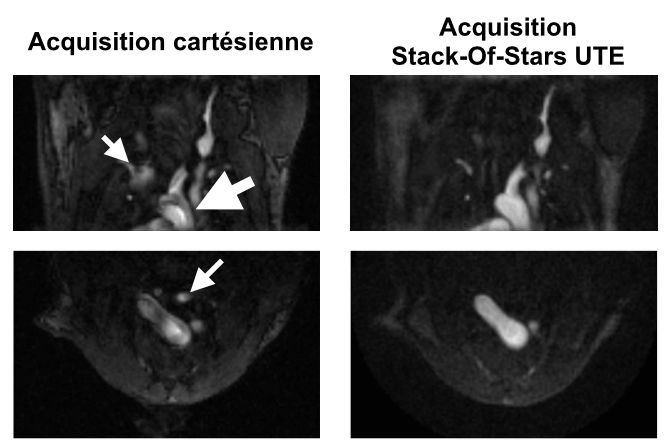
\includegraphics[scale=0.5]{./figure/chap2/Fig13.png}
\caption[Mouvements et imagerie radiale.]{\label{fig:MotionArt} \textbf{Mouvements et imagerie radiale.} Vue axiale des carotides d'une souris obtenue avec une séquence 3D PR à gauche et avec une séquence 3D cartésienne à droite. La flèche montre un artefact de flux sur l'image cartésienne qui correspond à une copie de la crosse aortique.}
\line(1,0){400} \\
\end{figure}

En imagerie radiale, les artefacts de mouvement se traduisent par du flou ou des artefacts de "streaking" qui se propagent perpendiculairement à la direction de lecture et qui sont éloignés de l'objet en mouvement d'une certaine distance, ce qui disperse l'erreur de manière plus ou moins homogène. Cette dispersion est encore plus efficace pour les séquences radiales 3D que 2D. Ces artefacts sont généralement moins dérangeants pour le diagnostic que les artefacts apparaissant en imagerie cartésienne (figure \ref{fig:MotionArt}).
Une deuxième raison expliquant la faible sensibilité aux mouvements pour l'imagerie radiale repose sur le sur-échantillonnage du centre de l'espace de Fourier grâce auquel un moyennage des projections contrebalance les erreurs enregistrées durant les phases de mouvement.
Ces deux propriétés réunies permettent d'expliquer le fort engouement des séquences 3D radiales pour l'imagerie d'organes en mouvement ou de patients peu coopératifs comme en pédiatrie \cite{block2014towards,Nayak:2014aa}.
Les séquences UTE bénéficient enfin d'un autre avantage car, après l'excitation, les spins sont déphasés puis rephasés par moins de gradient qu'avec des séquences cartésiennes. Cela permet de limiter les artefacts de déphasage de flux qui se traduisent par une absence de signal (figure \ref{fig:FluxArt}).

Pour toutes ces raisons, l'utilisation de séquences radiales est un choix intéressant en particulier pour des applications en angiographie et sur le petit animal. 
\begin{figure}[H]
\centering
\line(1,0){400} \\
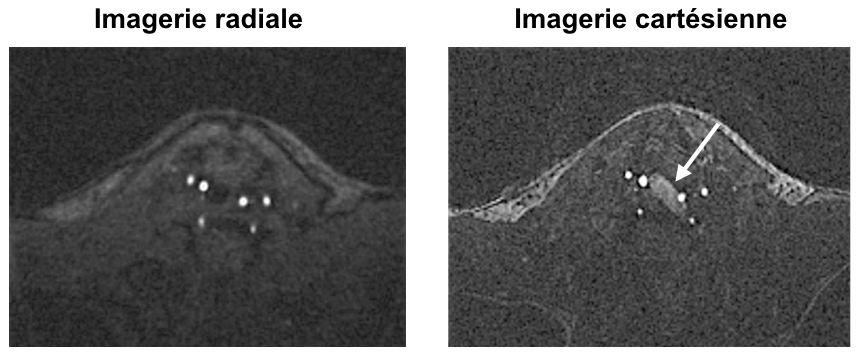
\includegraphics[scale=0.5]{./figure/chap2/Fig14.png}
\caption[Flux et imagerie radiale.]{\label{fig:FluxArt} \textbf{Flux et imagerie radiale.} Vue coronale (en haut) et axiale (en bas) de la crosse aortique d'une souris obtenues avec une séquence 3D cartésienne à gauche et avec une séquence 3D Stack-Of-Stars UTE à droite. Les deux acquisitions ont été effectuée sans synchronisation cardiaque ou respiratoire. La flèche épaisse montre une inhomogénéité du signal dans la crosse aortique qui sont des artefacts de déphasage du flux et les autres flèches  des artefacts de mouvement.}
\line(1,0){400} \\
\end{figure}

\subsubsection{Sur-échantillonnage en lecture}

Puisque l'espace de Fourier est échantillonné de manière discrète en IRM, la reconstruction de l'objet est périodique. C'est pour cela que l'on observe des effets de repliements de l'image si les points échantillonnés sont trop distants dans l'espace de Fourier et que les copies voisines se chevauchent dans le domaine image. Pour une résolution spatiale fixée, ce problème peut être éliminé en suréchantillonant la lecture, c'est-à-dire en utilisant une bande passante de réception plus grande. Cela permet donc d'augmenter le champ de vue mais aussi de compenser la diminution du rapport signal-sur-bruit induite par l'augmentation de la bande passante.

Pour l'imagerie cartésienne, cette possibilité de sur-échantillonnage est limitée à la direction de lecture car une augmentation du nombre de points dans les autres directions nécessitera l'acquisition de lignes supplémentaires. Pour l'imagerie radiale, cette limitation n'existe pas et le sur-échantillonnage peut être employé dans toutes les directions. C'est une particularité particulièrement  intéressante pour l'imagerie abdominale ou cardiaque \cite{block2014towards,Johnson:2012uq} où les régions d'intérêts sont localisées au centre. Cela permet de réduire le champ de vue nécessaire et donc de réduire le temps d'acquisition nécessaire.

\begin{figure}[H]
\centering
\line(1,0){400} \\
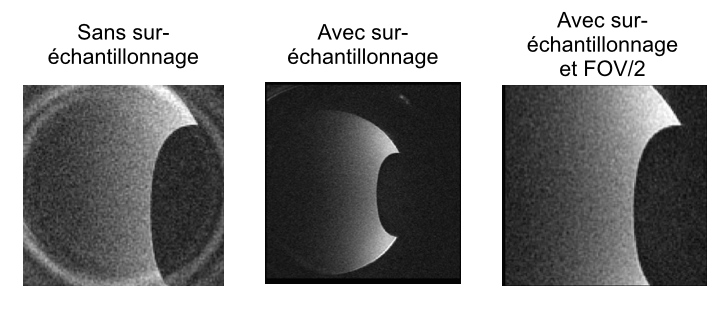
\includegraphics[scale=0.7]{./figure/chap2/Oversampling.png}
\caption[artefact de flux]{\label{fig:Oversampling} Vue axiale d'un fantôme. A gauche : Image acquise sans sur-échantillonnage (Nombre de points recueillis = 70 et bande passante de réception = 100 kHz). Au centre : Image acquise sans sur-échantillonnage (Nombre de points receuillies = 140 et bande passante de réception = 200 kHz). A droite : Image du centre coupé de manière à avoir la même dimension que celle de gauche. On observe que l'artefacts en cercle n'est plus présent sur l'image avec sur-échantillonnage ainsi qu'une amélioration du rapport signal-sur-bruit grâce à l'absence de repliement avec un champ de vue deux fois plus grand.}
\line(1,0){400} \\
\end{figure}

\subsubsection{Déviations des gradients}

Au cours des acquisitions IRM, les gradients de champ magnétique doivent rapidement monter puis descendre en intensité à de multiples reprises ce qui implique la création de courants de Foucault dans les bobines. Cela va modifier la trajectoire d'échantillonnage des points dans l'espace de Fourier.
Pour les séquences cartésiennes, cela ne pose pas de problème majeur car des formes de gradients identiques sont générées dans la direction de lecture pour toutes les répétitions. Cela résultera durant la reconstruction à une translation de la position des points échantillonnés selon la direction de lecture et donc à une modulation de phase dans le domaine image qui disparaitra lorsque l'image en magnitude sera calculée.

Cela est différent pour l'imagerie radiale car la direction de lecture varie pour chaque répétition. Dans cette situation, un simple délai de réponse des gradients cause une erreur non-uniforme de positionnement des points. Cela se traduit par des pertes de signal et du flou dans les images. C'est pour cela qu'il est nécessaire d'utiliser des méthodes de correction. Différentes techniques ont été proposées \cite{Alley:1998vn,Addy:2012kx} mais la méthode utilisée durant ces travaux de thèse est celle originellement décrite par Zhang et al \cite{Zhang:1998uq}.
Celle-ci consiste à mesurer le signal dans deux coupes positionnées symétriquement par rapport à l'isocentre, perpendiculairement à la direction du gradient. La phase du signal est extraite du signal puis déroulée pour éviter les repliements. La trajectoire dans l'espace selon cette axe est alors calculée en utilisant la phase des deux coupes. Cette méthode est reproduite sur chaque axe pour obtenir les trajectoires dans la $2^\text{ème}$ ou $3^\text{ème}$ dimension selon la séquence. Le chronogramme, la position des coupes et l'algorithme sont présentés dans la figure \ref{fig:SeqTraj}.

\begin{figure}[H]
\centering
\line(1,0){400} \\
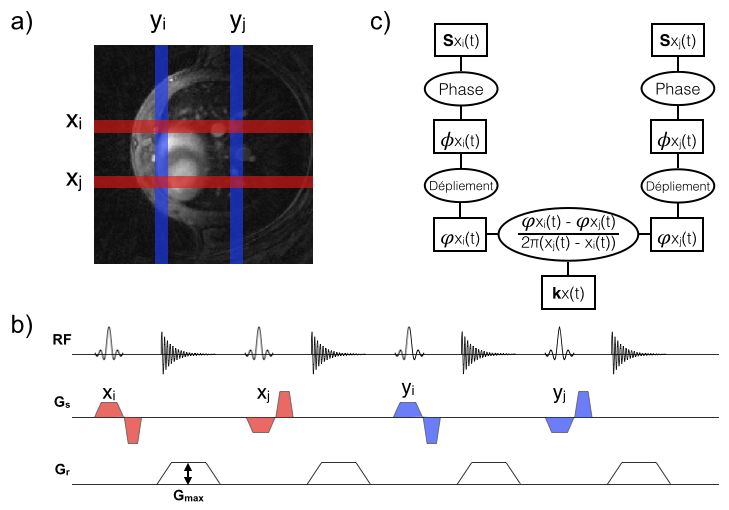
\includegraphics[scale=0.6]{./figure/chap2/SeqTraj.png}
\caption[Méthode mesure trajectoire]{\label{fig:SeqTraj}  
Mesure de trajectoire 2D UTE : (a) Positionnement des coupes de mesure symétriques par rapport à l'isocentre. (b) Chronogramme de la séquence utilisée. (c) Diagramme décrivant l'algorithme utilisé pour obtenir la trajectoire de l'axe verticale dans l'espace de Fourier à partir du signal dans les coupes $x_i$ et $x_j$.}
\line(1,0){400} \\
\end{figure}

\subsubsection{Sensibilité aux effets d'Off-Résonance}

En imagerie radiale les artefacts d'off-résonance sont différents de ceux en imagerie cartésienne. La variation d'évolution de la phase cause un déplacement des informations spatiales selon chaque orientation des projections qui crée donc un flou dans l'image (figure \ref{fig:OffRes}).
On peut distinguer plusieurs sources d'artefacts (la graisse, les effets de susceptibilité, l'inhomogénéité du champ statique, etc). La correction de ces artefacts a postériori n'est pas triviale et une stratégie plus rationnelle consiste à les réduire en modifiant la méthode d'acquisition avec :
\begin{enumerate}
\item Une augmentation de la bande passante de réception
\item L'utilisation de séquence à temps d'écho court
\item L'utilisation de séquence de type Echo de Spin
\end{enumerate}

Généralement, la principale source d'artefact d'off-résonance est la présence de graisse. En imagerie cardio-vasculaire sur petit animal, la graisse est peu présente autour des zones d'intérêt comme le cœur, la crosse aortique ou les carotides ce qui limite les artefacts. Cependant pour des méthodes nécessitant de longs temps d'écho, par exemple, pour obtenir un contrast $T_2^*$, l'imagerie radiale n'est pas conseillée et il est alors préférable d'utiliser une approche cartésienne ou bien une méthode de suppression de graisse (saturation, excitation sélective etc).
\begin{figure}[H]
\centering
\line(1,0){400} \\
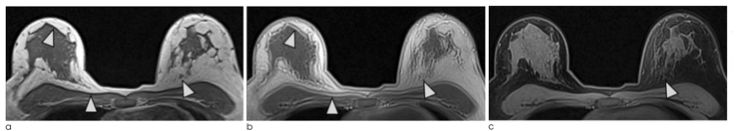
\includegraphics[scale=0.7]{./figure/chap2/OffRes.png}
\caption[artefact d'Off-résonance]{\label{fig:OffRes}  
(a) En imagerie cartésienne, la présence de graisse crée un artefact de déplacement chimique dans la direction de lecture. (b) A cause de la modification de l'orientation de la direction de lecture en imagerie radiale, les artefacts apparaissent comme un flou entourant les zones graisseuses. (c) Ces artefacts peuvent être éliminés en utilisant une méthode de suppression de graisse. Figure extraite d'un article de Block et Al. (JKSMRM 2014)}
\line(1,0){400} \\
\end{figure}

\section{Résumé}

Avec un schéma d'acquisition radiale, les données de l'espace de Fourier sont recueillies selon des projections plutôt que des lignes parallèles. La modification d'une séquence cartésienne existante en une séquence radiale peut généralement être facilement effectuée que ce soit en 2D ou en 3D. Cependant, à cause de la position non équidistante des points, une méthode de reconstruction spéciale doit être utilisée comme le remaillage des données.

L'imagerie radiale dispose de plusieurs avantages par rapport à une acquisition cartésienne comme une faible sensibilité aux artefacts de flux et de mouvement, la possibilité de sur-échantillonner l'acquisition dans toutes les directions sans augmenter le temps d'acquisition requis ce qui élimine les artefacts de repliement. De plus, le centre de l'espace de Fourier est sur-échantillonné, ce qui autorise alors un intéressant sous-échantillonnage de l'acquisition. Bien que l'acquisition d'un nombre réduit de projections puissent créer des artefacts de "streaking", une grand partie des informations de l'objet reste visible même avec un fort facteur d'accélération, ce qui n'est pas le cas avec une trajectoire cartésienne. De plus, chaque projection acquière un niveau équivalent d'information de haute et de basse fréquences, ce qui offre une mise à jour des informations plus homogène pour des applications en temps réel ou dynamique en IRM.

D'un autre côté, le nombre de projections à recueillir pour obtenir un espace de Fourier complet est plus important qu'en imagerie cartésienne ce qui peut prolonger le temps d'acquisition. L'imagerie radiale est aussi plus sensible aux déviations des valeurs des gradients, bien qu'aujourd'hui cela soit un problème moins important avec les systèmes récents d'IRM. Le principal problème de cette méthode est sa sensibilité aux artefacts de déphasage et en particulier de déplacement chimique. C'est pourquoi l'utilisation de séquence radiale n'est pas recommandée pour obtenir un contraste $T_2^*$.


%\chapter{Développement d'une méthode d'angiographie dynamique avec une séquence d'imagerie radiale à encodage pseudo-aléatoire par un double angle d'or ciné.}
\setlength{\footskip}{50pt}
\chaptermark{Angiographie dynamique avec double angle d'or}

\label{Chap3}
\section{Contexte}

Dans de nombreuses pathologies vasculaires, l’intégrité physique du vaisseau est touchée. Afin de visualiser les vaisseaux de manière non invasive, l’Angiographie par Résonance Magnétique (ARM) est devenue une technique de référence en clinique. Elle permet en effet d’apprécier l’anatomie des vaisseaux et visualiser les déformations de ces derniers (sténose, anévrisme, …). Néanmoins, dans de nombreuses pathologies, ou dans le cas d’un diagnostic précoce, l’imagerie anatomique n’est pas un examen suffisant et les informations obtenues apparaissent normales. Il apparait donc intéressant de développer des méthodes d'investigation fonctionnelles, permettant de visualiser et quantifier le flux sanguin dans les vaisseaux. Pour obtenir ces informations, il est nécessaire de recueillir des images à la fois en trois dimensions et résolues dans le temps. On parle alors d’angiographie 4D.

Les problématiques que l'on peut rencontrer chez le petit animal ne sont pas les mêmes que chez l'humain ce qui limite l'utilisation de certaines séquences ou nécessite une adaptation. L'une des limitations principales pour effectuer la mesure de flux chez la souris est son rythme cardiaque supérieur à 400 battements par minutes lorsque celle-ci est anesthésiée. La résolution temporelle de la séquence doit dont être importante pour obtenir une bonne visualisation de la dynamique des flux. Afin d’apprécier la vitesse du sang dans les vaisseaux plusieurs méthodes sont disponibles en IRM chez l’homme : 
\begin{itemize}
\item L’imagerie de prise de contraste du Gadolinium. Pour cette technique, les acquisitions sont faites assez rapidement pour visualiser l’arrivée du produit dans lez zones d’intérêt. Aujourd’hui, avec les progrès instrumentaux et méthodologiques, il est possible d’obtenir des images sub-millimétriques en moins d’une seconde \cite{Wu:2011ys}. Ces méthodes sont aujourd’hui les méthodes de référence chez l’homme. En revanche, leurs transfert chez le petit animal apparaît difficile voir impossible compte tenu de la taille des vaisseaux observés et de la cinétique de biodistribution des agents de contraste (moins de 2 secondes pour le premier passage d’un agent de contraste classique à base Gadolinium).

\item L’imagerie 4D par contraste de phase \cite{Markl:2012pi}. Cette méthode est aujourd’hui de plus en plus répandue en clinique et a permis d’étudier de nombreuses pathologies comme les complications après la réparation d'un anévrisme ou d'une dissection de l'aorte \cite{frydrychowicz2011aortic} , des pathologies associées aux remplacements des valves aortiques \cite{kvitting2004flow} ou bien pour étudier l'hypertension pulmonaire artérielle \cite{sanz2007pulmonary}.
Grâce à l’application d’un gradient bipolaire de durée et d’intensité déterminées, le déphasage des spins est alors proportionnel à la vitesse du flux. Cette méthode a pour principal avantage d’offrir une visualisation de la vitesse et de la direction du flux voxel par voxel. Toutefois, l’inconvénient majeur de cette technique est son temps d’acquisition long puisqu’il est nécessaire de répéter la séquence 4 fois pour encoder la vitesse dans toutes les directions \cite{Johnson:2010uq,Robson:2010uq,Wu:2013ys}. 
Chez le petit animal, une fois de plus, compte tenu de la taille des zones à observer, du manque de rapport signal-sur-bruit, ce type d’acquisition de mesure des flux est peu répandu. En imagerie 2D seules quelques publications ont montré le potentiel de la méthode, et à notre connaissance en imagerie 3D+t, seule une publication est rapportée \cite{Janiczek:2011qm}.

\item L’imagerie par marquage de spin. Cette méthode permet d’estimer la vitesse des flux grâce à des acquisitions multiples avec ou sans marquage des spins sanguins puis une soustraction des images obtenues (Koktzoglou and Edelman \cite{Koktzoglou:2009fe}). Le desavantage de cette méthode est qu’elle necessite deux acquisitions, donc un temps d’acquisition relativement important.
Une méthode alternative basée sur l’imagerie ciné temps-de-vol (Time-Of-Flight : TOF) a été développée au sein du laboratoire par  Miraux et al. \cite{Miraux:2006fu} et appliquée chez le petit animal. Celle-ci consiste, après la détection d’un pic ECG, à saturer le signal dans le volume d'imagerie puis à recueillir le signal du sang frais progressant dans les vaisseaux (voir figure \ref{fig:SeqSylvain}) à l’aide de séquences ciné 3D.
\end{itemize}

\begin{figure}[H]
\centering
\line(1,0){400} \\
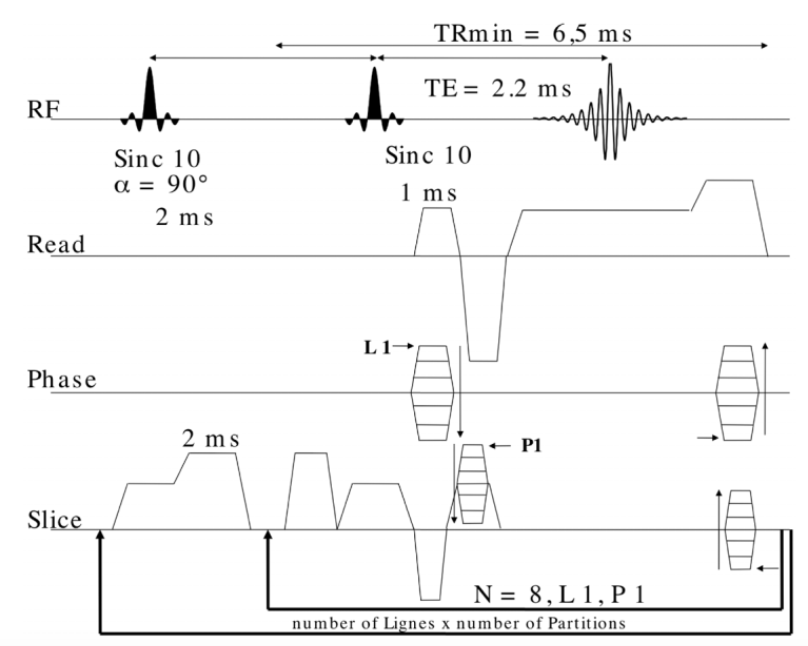
\includegraphics[scale=0.5]{./figure/chap3/SeqSylvain.png}
\caption[Séquence d'angiographie dynamique.]{\label{fig:SeqSylvain} \textbf{Séquence d'angiographie dynamique.} Chronogramme de la séquence utilisée pour obtenir une ARM "sang-blanc" résolue dans le temps. L = Nombre de ligne, P = Nombre de partition, N = Nombre d'images résolues dans le temps reconstruites. (Figure extraite de Miraux et al. 2006 \cite{Miraux:2006fu})}
\line(1,0){400} \\ \end{figure}

La méthode d'imagerie de flux par temps-de-vol a permis de mesurer les flux sanguins dans diverses artères chez la souris : carotides \cite{Miraux:2006fu}, pulmonaires \cite{Cochet:2013dk} et même coronaires \cite{Cochet:2010ec} ainsi que dans le polygone de Willis.

Néanmoins, le temps d’acquisition pour cette angiographie ciné 3D reste long, en particulier lorsqu’il est nécessaire d’obtenir des images avec des résolutions spatiale et temporelle élevées. Pour réduire ces temps d’acquisition, les techniques d’imagerie parallèle peuvent être utilisées mais avec le matériel disponible en imagerie pré-clinique un gain maximum d’un facteur 2 peut être atteint et ceci au détriment du rapport signal-sur-bruit. 

C’est pourquoi, il a été choisi de s'orienter vers une autre stratégie afin de diminuer les temps d’acquisition de manière significative. Cette stratégie se base sur les techniques d’acquisition radiale parce qu’elles permettent en théorie d’obtenir de forts facteurs de sous-échantillonnage. Elles sont également extrêmement flexibles et adaptables aux méthodes de rehaussement de résolution spatiale de type fenêtre glissante.

Le but des travaux présentés dans ce chapitre est donc de combiner la méthode d’angiographie dynamique par temps-de-vol avec des trajectoires 3D radiales afin de générer des images à fortes résolutions spatiale et temporelle rapidement. Pour cela nous avons mis au point une méthode originale d’encodage doublement pseudo-aléatoire.


\section{Angiographie à partir de séquence radiale.}

L'un des inconvénients de la trajectoire cartésienne est son manque de flexibilité dans la reconstruction de l'image. Une fois que la résolution temporelle a été déterminée par le nombre de lignes successives à recueillir pour chaque répétition, il est difficile d'obtenir des images de bonne qualité (à partir du même jeu de donnée) avec une résolution temporelle différente.
Les trajectoires radiales sont plus flexibles car elles permettent de reconstruire des images intermédiaires sans attendre d'avoir recueilli toutes les projections de l'espace de Fourier. Mais, comme montré dans la figure \ref{fig:SousEchan}, cela est très dépendant de la méthode de répartition des projections qui est employée. La répartition linéaire permet d'obtenir une répartition homogène des projections lorsque toutes les données sont recueillies mais elle manque de flexibilité lors de la reconstruction d'une image n'utilisant seulement qu'une partie des données recueillies durant un temps donné. Il est donc nécessaire de proposer des répartitions pseudo-aléatoires qui permettront de répartir de manière plus homogène les projections au cours du temps et donc d'obtenir des images de meilleure qualité par exemple dans la figure \ref{fig:SousEchan}.droite.

De nombreuses méthodes de répartition pseudo-aléatoire des projections 2D et 3D ont été étudiées : les méthodes utilisant des trajectoires multi-spirale \cite{Chan:2009uq}, la méthode quasi-"random" \cite{Tibiletti2015Multistage-thre}, les méthodes d'inversion de bit \cite{Theilmann2004View-ordering-i}, les séquences Halton \cite{chan2009halton} ou bien encore des méthodes utilisant l'angle d'or\cite{Winkelmann:2007fk}. Winkelmann et al. \cite{Winkelmann:2007fk} et Song et al. \cite{Song:2000fk} ont montré que l'imagerie radiale 2D est plus flexible en utilisant un angle d'or, dérivé du facteur d'or (décrit dans la prochaine section). Par exemple en imagerie de prise de contraste dynamique, en positionnant les projections dans l'espace de Fourier avec cet angle, il est possible à partir de n'importe quelle position de reconstruire une image. Le nombre de projection à utiliser peut être adapté à la résolution spatio-temporelle souhaitée. Chan et al. \cite{Chan:2009uq} ont montré qu'il était possible d'étendre la notion d'angle d'or à l'imagerie radiale 3D et ont montré son application à l'imagerie dynamique de prise de contraste dans les tumeurs du sein.

La méthode se basant sur l’angle d’or a été privilégiée dans les travaux montrés ici.

\begin{figure}[H]
\centering
\line(1,0){400} \\
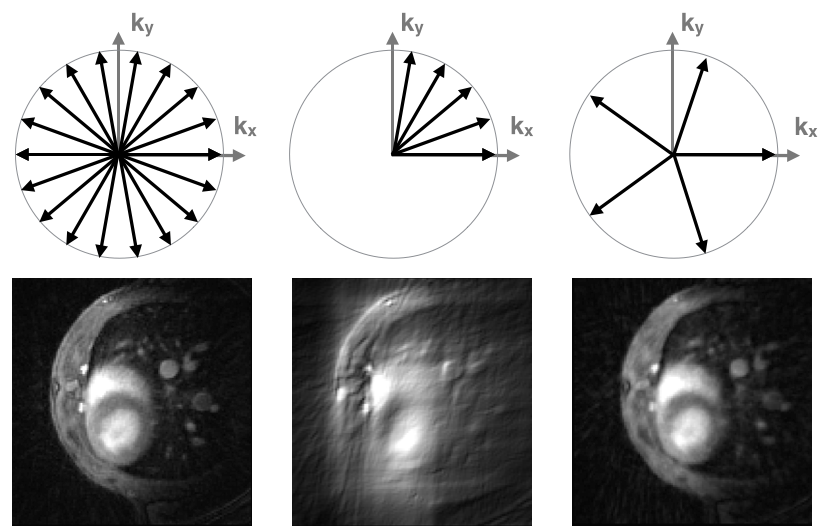
\includegraphics[scale=0.5]{./figure/chap3/SousEchan.png}
\caption[Homogénéité de répartition des projections.]{\label{fig:SousEchan} \textbf{Homogénéité de répartition des projections.} Vues axiales obtenues avec une séquence UTE 2D sur le coeur de souris en fonction de la répartition des projections dans l'espace de Fourier. A gauche : l'image est reconstruite avec les 402 projections réparties de façon homogène dans l'espace de Fourier pour atteindre le critère de Nyquist. Au centre : l'image est acquises avec 100 projections réparties de manière adjacente. A droite : l'image est reconstruite avec 100 projections réparties de manière uniforme sur le plan.}
\line(1,0){400} \\ \end{figure}

\subsection{Angle d'or}

L'angle d'or $\phi$ est dérivé du facteur d'or qui est extrait de la suite de Fibonacci. Il est utilisé en IRM pour de nombreuses applications permettant de répartir au mieux des données dans l'espace de Fourier. En imagerie radiale 2D, cet angle d'or $\phi$ est égale à $111,24 \degres$. Chaque projection est donc séparée de la précédente par cet angle $\phi$. Cela a pour effet de bien répartir spatialement et temporellement les projections au cours du temps (figure \ref{fig:Gold2D})

\begin{figure}[h]
\centering \line(1,0){400} \\
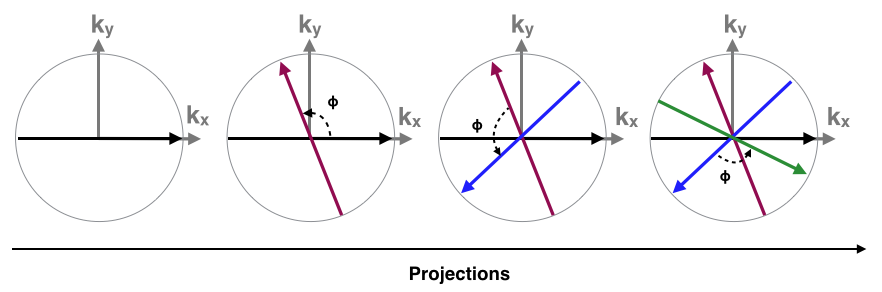
\includegraphics[scale=0.7]{./figure/chap3/Gold2D.png}
\caption[Angle d'or 2D.]{\label{fig:Gold2D} \textbf{Angle d'or 2D.}  Répartitions des projections radiales dans l'espace de Fourier basé sur l'angle d'or 2D.}
\line(1,0){400} \\ \end{figure}

\begin{figure}[h]
\centering \line(1,0){400} \\
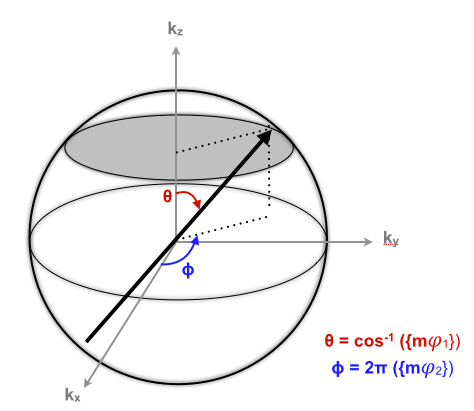
\includegraphics[scale=0.4]{./figure/chap3/Gold3D.png}
\caption[Angle d'or 3D.]{\label{fig:Gold3D} \textbf{Angle d'or 3D.} Positionnement des projections radiales dans l'espace de Fourier basé sur l'angle d'or 3D.}
\line(1,0){400} \\ \end{figure}

Ce principe d'angle d'or a été étendu à l'imagerie 3D. Deux facteurs d'or sont nécessaires à son implémentation ($\phi_1=0,4656$=,$\phi_2=0,6823$). Ici, la méthode de répartition des projections employée pour l'imagerie 3D utilise $\phi_1$ pour orienter la projection d'un angle $\phi$ par rapport à l'axe $k_z$ et $\phi_2$ pour déterminer l'angle polaire $\theta$ de la projection dans le plan $(k_x,k_y)$ (figure \ref{fig:Gold3D}) selon les équations suivantes :
\begin{equation}
\label{eq:GoldPremier}
\begin{array}{c}
\Phi_i=2\pi \times mod(\phi_1 \times i,1) \\
\theta_i=2 \times acos(mod(\phi_2 \times i,1)) -1
\end{array}
\end{equation}
où i est le numéro de la projection. Comme montré dans la figure \ref{fig:ComparTraj}, on observe que la répartition des projections au cours du temps est uniforme dans l'espace.

\begin{figure}[h]
\centering \line(1,0){400} \\
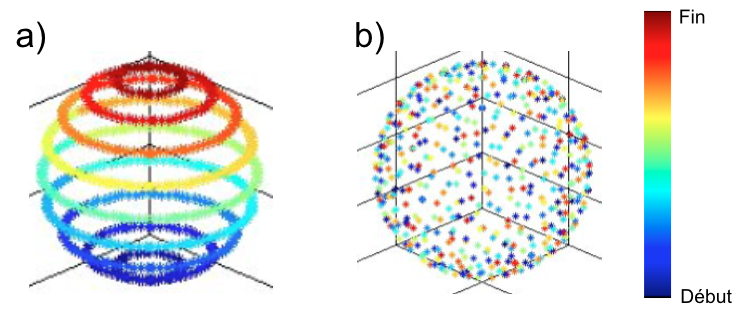
\includegraphics[scale=0.4]{./figure/chap3/ComparTraj.png}
\caption[Comparaison du positionnement des projections au cours du temps.]{\label{fig:ComparTraj} \textbf{Comparaison du positionnement des projections au cours du temps.} Positionnement des derniers points de chaque projection radiale dans l'espace de Fourier au cours du temps selon les méthodes : (a) utilisée sur les imageurs Brüker (b) méthode basée sur l'angle d'or 3D.}
\line(1,0){400} \\ \end{figure}

\subsection{Angiographie anatomique avec l'angle d'or et sous-échantillonnage}

Des images d'angiographie temps-de-vol au niveau des carotides de plusieurs souris ont été acquises avec une séquence d'imagerie radiale 3D et une répartition des projections à l'aide de l'angle d'or. Le nombre de projections utilisé au départ (40 000) pour reconstruire les images a ensuite été réduit à 8 000, 4 000 et 2 500. Ces images ont été comparées qualitativement à une image obtenue avec un encodage cartésien.

\begin{figure}[H]
\centering \line(1,0){400} \\
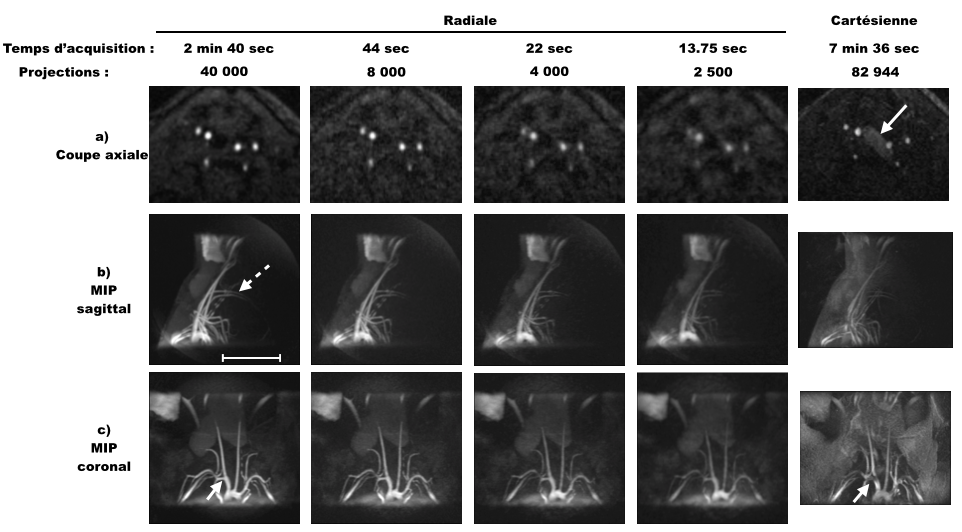
\includegraphics[scale=0.5]{./figure/chap3/RadialAnat.png}
\caption[Sous-échantillonnage en imagerie radiale 3D avec l'angle d'or 3D.]{\label{fig:RadialAnat} \textbf{Sous-échantillonnage en imagerie radiale 3D avec l'angle d'or 3D.}  Coupe axiale et projections d'intensité maximale (sagittale et coronales) issues d'une imagerie anatomique 3D positionnée au niveau des carotides d'une souris en acquisition radiale et cartésienne. Le nombre de projection utilisée en méthode radiale est de 40 000, 8 000, 4 000 et 2 500 projections. La barre d'échelle correspond à une longueur de 10 mm. }
\line(1,0){400} \\ \end{figure}

Comme on peut le voir sur la figure \ref{fig:RadialAnat}, malgré des facteurs de sous échantillonnage importants en imagerie radiale (5, 10, 16) la plupart des gros vaisseaux sont visibles sur les images avec aussi bien 8 000, 4 000 que 2 500 projections. Néanmoins, l’effet du fort sous-échantillonnage se traduit par une difficulté à distinguer les parties des artères les plus petites en taille sur les images d’intensité de projection maximale (MIP) comme indiqué par la flèche en pointillée. Cependant, l’angiogramme complet est bien défini avec seulement 4 000 projections correspondant à un temps d’acquisition de 22 secondes. 
Sur les images recueillies avec la séquence cartésienne, en dépit d’un temps d’acquisition beaucoup plus élevé, de nombreux artéfacts sont observés. On distingue en effet la présence du repliement de la crosse aortique provoqué par un artéfact de flux sur l’image axiale qui n’est pas présent en imagerie radiale. Le signal du sang apparaît moins important et moins homogène que sur les images radiales en particulier au niveau des flux turbulents comme montré par la petite flèche blanche.
L’acquisition de ces images anatomiques a permis de montrer la robustesse aux artéfacts de flux et de mouvement des séquences radiales en comparaison avec les séquences cartésiennes.  
L’utilisation de l’angle d’or 3D permet de répartir l’information uniformément en fonction du temps dans l’espace de Fourier et ainsi obtenir des images de qualité dans un temps restreint.

\section{Angiographie radiale résolue dans le temps.}

\subsection{Séquence}

La séquence d’imagerie radiale utilisée pour la visualisation du flux chez le petit animal est montrée en figure \ref{fig:SeqARMAurel}. Elle est basée sur la séquence publiée en 2006 par Miraux et al. \cite{Miraux:2006fu}. Elle est constituée, en amont, d'un module de saturation sélectif du volume d'imagerie. Après ce module, une séquence d'écho de gradient 3D rapide est appliquée et répétée un nombre de fois N correspondant au nombre d'images ciné que l'on souhaite reconstruire. Cette séquence d'écho de gradient est constituée d'une impulsion radiofréquence sélective dans l'espace permettant d'obtenir un signal temps-de-vol dans le volume imagé. L'impulsion est suivie d'un gradient de rephasage de coupe combiné à des gradients de déphasage selon les trois axes permettant de se déplacer vers l'extérieur de l'espace de Fourier. Les gradients sont ensuite inversés pour permettre la lecture du signal selon une projection donnée. 
L'intensité des gradients sur les axes x, y et z est modulée en fonction du numéro de la trajectoire à recueillir, ici noté i, et déterminée grâce à un calcul préalable des coordonnées $kx_i$, $ky_i$ et $kz_i$ du point de départ de la projection. Ces coordonnées sont données par les équations suivantes :
\begin{equation}
\label{eq:GoldSecond}
\begin{array}{c}
kx_i = kmax \times \cos(\Phi_i) \sin(\theta_i) \\
ky_i = kmax \times \sin(\Phi_i) \sin(\theta_i) \\
kz_i = kmax \times \cos(\theta_i)
\end{array}
\end{equation}
où $\Phi_i$ et $\theta_i$ sont obtenues grâce à l'équation \ref{eq:GoldPremier} définissant les trajectoires selon l'angle d'or 3D. Des gradients de "spoiling" sont ensuite appliqués pour déphaser le signal résiduel à chaque TR.

\begin{figure}[H]
\centering \line(1,0){400} \\
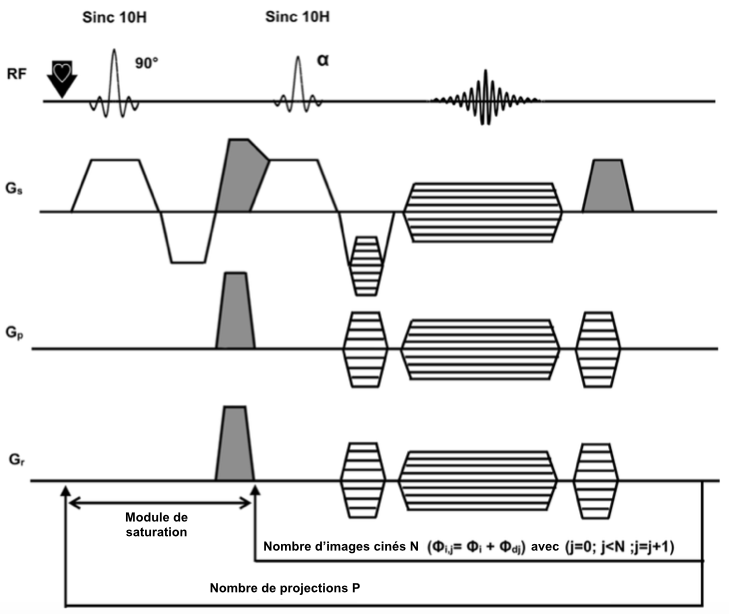
\includegraphics[scale=0.5]{./figure/chap3/SeqARMAurel.png}
\caption[Chronogramme de la séquence ARM sang blanc 3D radiale synchronisée sur l'ECG.]{\label{fig:SeqARMAurel}\textbf{ Chronogramme de la séquence ARM sang blanc 3D radiale synchronisée sur l'ECG.} Un module de saturation a été ajouté avant l'acquisition de N images cinés. Chacune de ces images a été acquises avec $P(\Phi_{i,j},\theta_i)$ projections. Pour chaque image ciné, $\Phi_{i,j} = \Phi_i+\Phi d_j$, où i est le nombre de projection et j est le nombre de ciné. Les gradients de déphasage sont indiqués en gris. La flèche noire représente la synchronisation ECG.}
\line(1,0){400} \\ \end{figure}

\subsection{Second angle d'or}

Généralement en imagerie résolue dans le temps, N signaux IRM sont recueillis successivement avec la même trajectoire dans l'espace de Fourier. Cela est répété de manière à pouvoir remplir N espaces de Fourier complets afin de pouvoir reconstruire N images (souvent appelé image ciné). Lorsque les temps de répétition sont courts par rapport aux mouvements que l'on souhaite observer, la différence entre les images est très faible et l'on obtient donc une redondance importante dans les informations contenues dans l'espace de Fourier. Or, comme expliqué dans la section \ref{subsec:KSpaceRegion}, il est possible d'exploiter les hautes fréquences pour augmenter la résolution de l'image. Cependant la méthode standard d'imagerie résolue dans le temps ne permet pas de flexibilité spatiotemporelle entre les différentes images reconstruites. Cette propriété est présente que l'on utilise des trajectoires cartésiennes ou non-cartésiennes car il provient seulement du fait que les trajectoires utilisées entre les images ciné sont les mêmes. Pour résoudre ce problème, il est donc nécessaire de modifier les trajectoires entre les images ciné de manière à pouvoir ensuite les manipuler par exemple en additionnant deux espaces de Fourier ce qui permet de gagner en résolution spatiale et en signal mais réduit la résolution temporelle. 

La méthode choisie a été de recueillir le signal de chaque moment du cycle cardiaque avec des trajectoires similaires mais subissant une rotation autour de l'axe $k_z$. L'angle employée, noté $\Phi d_j$ est aussi basé sur l'angle d'or 2D $v_2$ et s'intègre dans les équations précédentes de la manière suivante :
\begin{equation}
\begin{array}{c}
\Phi_i=2\pi \times mod(\phi_1 \times i,1) +\Phi d_j\\
\theta_i=acos(mod(\phi_2 \times i,1)) \\
avec\ \ \Phi d_j=2\pi \times  mod( v_2 \times j)
\end{array}
\end{equation}
où j correspond au numéro de l'espace de Fourier du cycle cardiaque qui sera complété par cette projection. Cette méthode permet donc d'obtenir une répartition des projections similaire mais avec des trajectoires d'échantillonnage de l'espace de Fourier différentes (figure \ref{fig:GoldCine}) en fonction de la position dans le cycle cardiaque. Cette méthode est plus efficace qu'une simple rotation de la trajectoire d'un angle (360/Nombre d'images cinés) car, lors de la reconstruction, les espaces de Fourier ainsi recueillis seront très proches. Il est au contraire intéressant d'avoir un angle plus élevé qui permettra d'obtenir des trajectoires très différentes sur les cinés adjacentes plutôt que des trajectoires proches qui donneront peu de nouvelles informations pour améliorer la résolution spatiale. 
L'implémentation de ces trajectoires dans une séquence d'ARM dynamique de flux est décrite dans la figure \ref{fig:SeqARMAurel} sous forme de chronogramme.
 
\begin{figure}[H]
\centering \line(1,0){400} \\
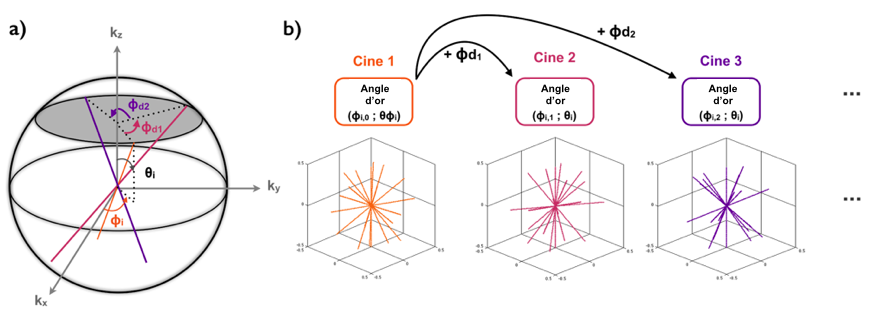
\includegraphics[scale=0.5]{./figure/chap3/GoldCine.png}
\caption[Répartition grâce à l'angle d'or entre les images cinés.]{\label{fig:GoldCine} \textbf{Répartition grâce à l'angle d'or entre les images cinés.} Description de la méthode utilisée pour obtenir une répartition différente des projections entre des images ciné consécutives. (a) Le segment orange représente la trajectoire d'une projection définie par le premier angle d'or, correspondant à l'image ciné 1 . Pour l'image ciné 2 (rose), la nouvelle trajectoire est obtenue en ajoutant l'angle $\Phi d_1$. Pour l'image ciné 3 (violet), l'angle ajouté est égale à $\Phi d_2$. La même valeur d'angle $\theta_i$, est utilisée entre les projections des images ciné adjacentes. (b) Exemple sur la distribution 9 projections pour 3 images ciné consécutives.}
\line(1,0){400} \\ \end{figure}

\subsection{Filtre temporel}

Grâce à la méthode d’encodage doublement pseudo-aléatoire implantée, il est possible, a posteriori, d’utiliser un filtre temporel pour reconstruire une image ciné à un temps donné du cycle cardiaque. Ce filtre temporel permet de regrouper les données de l'espace de Fourier que l'on veut reconstruire avec une partie des hautes fréquences des espaces de Fourier adjacents. De nombreux filtres différents peuvent être créés et adaptés a posteriori lors de la reconstruction comme des filtres exponentiels ou linéaires qui s'utilisent pour des images de prises de contraste dynamiques \cite{Lin:2008uq}.
Il a ici été décidé d'utiliser un filtre défini par 2 paramètres, Q et R ($Q \leq R$) qui correspondent à des distances temporelles entre les espaces de Fourier dans le cycle cardiaque par rapport à l'espace de Fourier à reconstruire. Pour reconstruire l'image située à la position x du cycle cardiaque, tout l'espace de Fourier à cette position sera utilisé auquel sera ajouté la moitié des hautes fréquences des espaces situés à une position s tel que : $x-Q < s \leq x+Q$. Et enfin il sera également ajouté le quart des hautes fréquences des espaces de Fourier situés à une position $x-Q-R \leq s < x-Q$ et $x+Q \geq s \geq x+Q+R$. La forme de ce filtre est illustrée dans la figure \ref{fig:filtre} pour des valeurs R = 3 et Q = 1.
La résolution temporelle est donc étalée sur 7 TR mais le fait de ne pas utiliser les basses fréquences dans les images ciné adjacentes permet de réduire la résolution temporelle effective.
Après application du filtre temporel, on obtient un espace de Fourier que l'on peut exploiter avec la méthode de remaillage des données ("gridding") standard décrit dans le chapitre précédente.
L'utilisation d'un filtre temporel n'est pas uniforme sur tout le cycle cardiaque. En effet, des effets de bords réduiront la qualité des images que l'on peut obtenir au début et à la fin du cycle cardiaque.

\begin{figure}[H]
\centering \line(1,0){400} \\
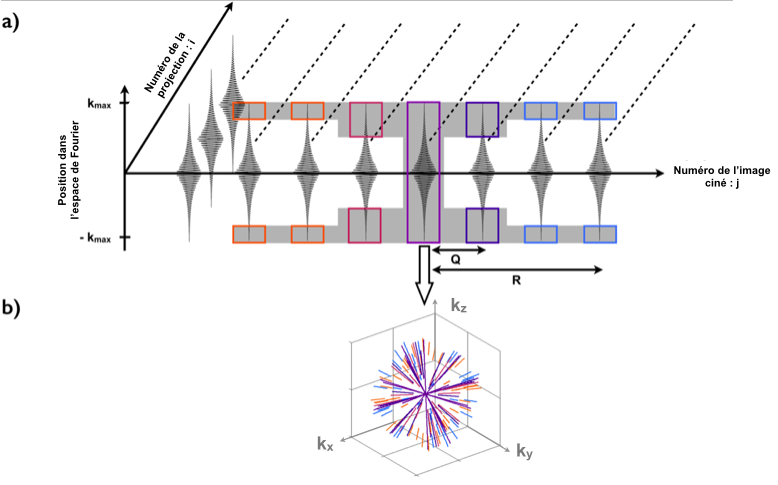
\includegraphics[scale=0.45]{./figure/chap3/filtre.png}
\caption[Exemple de filtre temporel.]{\label{fig:filtre} \textbf{Exemple de filtre temporel.} Représentation du filtre temporel (en gris) utilisé pour reconstruire l'image ciné 5 avec Q = 1 et R = 3. (a) Les données sont reconstruites en utilisant la moitié des hautes fréquences des projections recueillies à une distance temporelle maximum Q, et un quart des projections receuillies à des distances temporelles plus élevées (de Q à R). (b) Représentation schématique de l'espace de Fourier de l'image ciné 5 après application du filtre temporel.}
\line(1,0){400} \\ \end{figure}

\subsection{Résultats}

Toutes les expériences décrites dans cette partie ont été effectuées sur un imageur 7T Brüker Biospec (Ettlingen, Allemagne) équipé avec un système de gradient capable de fournir 660 mT/m au maximum et avec un temps de montée des gradients de 110 $\mu$s.
Une antenne volumique quadratique (Diamètre interne 75.4 mm, longueur = 70 mm) est utilisée pour l'excitation et une antenne de surface à 4 éléments (dimension extérieure d'un élément d'antenne: 12 $\times$ 16 mm$ ^2$; dimension extérieure totale: 26 $\times$ 21 mm$ ^2$) est utilisée pour la réception du signal.

\subsubsection{Validation de la séquence sur fantômes}

La séquence a tout d'abord été validée sur un fantôme de flux, en particulier l'effet du sous-échantillonnage et l'utilisation du filtre temporel sur l'évaluation de la dynamique de progression des flux. Pour cela, un fantôme constitué de spins stationnaires contenus dans un cylindre rempli avec de l'eau et de spins mobiles dans un tube rectiligne contenant de l'eau a été imagé. Le diamètre du tube est de 0,5 mm et le débit de l'eau dans le tube est de 3,75 mL/min qui correspond à une vitesse moyenne de 31,8 cm/s à l'intérieur du tube. La séquence n'est pas synchronisée et 20 images cinés sont recueillies. Les paramètres utilisés pour l'imagerie sont les suivants : TE/TR = 1,5/3,3 ms; $\alpha=12\degres$; bande passante de réception = 200 kHz; Champ-de-vue = $25 \times 25 \times 25 mm^3$; matrice reconstruite = $192 \times 192 \times 192$; résolution spatiale = $(130 \ \mu m)^3$.
\begin{figure}[H]
\centering \line(1,0){400} \\
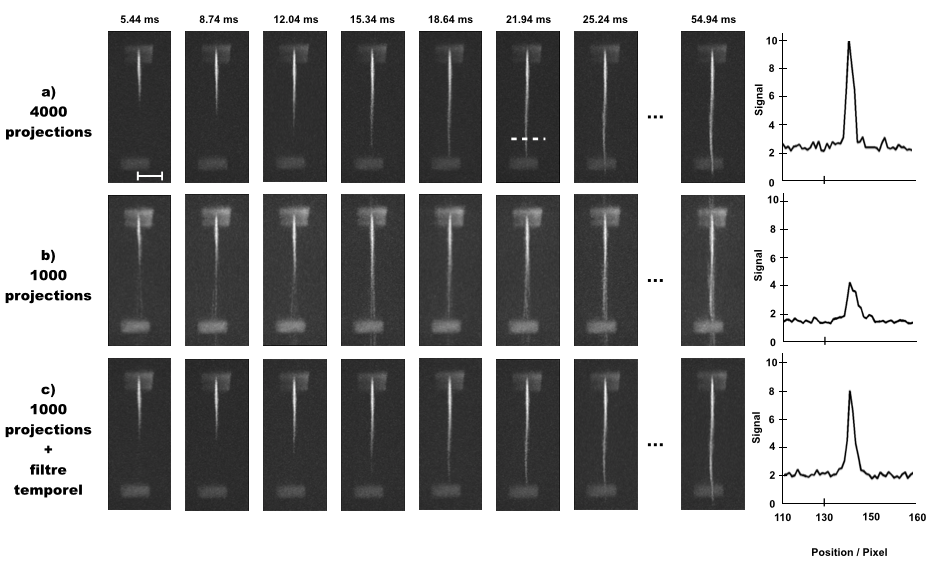
\includegraphics[scale=0.5]{./figure/chap3/ImFlowPhant.png}
\caption[IImagerie de flux dynamique in vitro.]{\label{fig:ImFlowPhant} \textbf{Imagerie de flux dynamique in vitro.} Images MIP coronales recueillies sur le fantôme de flux avec la séquence dynamique. Les images reconstruites avec (a) 4 000 ou (b) 1 000 projections sont comparées aux images reconstruites avec (c) 1000 projections et l'utilisation d'un filtre temporel (R=3, Q=1). Le profil d'intensité est obtenu au niveau de la ligne en pointillée au temps 21,94 ms pour chaque cas. La barre d'échelle correspond à une longueur de 5 mm.}
\line(1,0){400} \\ \end{figure}

Les données sont sous-échantillonnées a posteriori pour obtenir un jeu de donnée constitué de 1000 et 4000 projections correspondant respectivement à des temps d'acquisition de 4 min 51 s et 1 min 13 s. Avec 4 000 projections (figure \ref{fig:ImFlowPhant}.a), il est possible de visualiser distinctement la progression du flux dans le tube et sa vitesse peut être correctement mesurée. La vitesse maximum observée est égal à 65 cm/s, ce qui correspond logiquement à 2 fois la valeur moyenne. Avec 1 000 projections (figure \ref{fig:ImFlowPhant}.b), on observe sur les images une nette infériorité en terme de signal et de résolution spatiale. Le signal sur bruit du tube passe de 10 à 4,2 entre 4 000 et 1 000 projections. On observe aussi la présence d'artéfacts de streaking qui empêche la mesure d'une valeur précise de vitesse des flux. Cependant en utilisant le filtre temporel (R=3,Q=1) (figure \ref{fig:ImFlowPhant}.c) les artéfacts de streaking sont supprimés et l'on observe que le profile de signal remonte de 4.2 à 8.
L'augmentation du volume de flux dans le champ de vue a été mesuré sur toutes les images ciné (correspondant à la progression du flux dans le tube) et l'on observe une sur-évaluation du volume sur les images reconstruites avec 1000 projections (\ref{fig:GraphFlowPhant}.1). En revanche, avec l'utilisation du filtre on observe des données totalement en accord avec celles reconstruites avec 4000 projections.

\begin{figure}[H]
\centering \line(1,0){400} \\
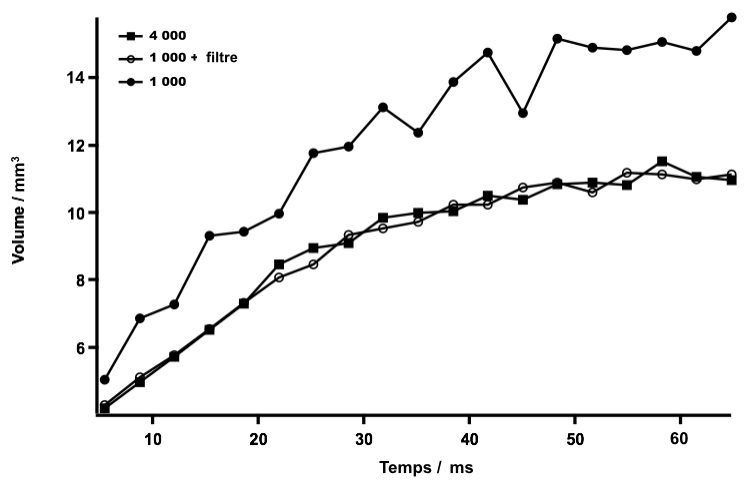
\includegraphics[scale=0.4]{./figure/chap3/GraphFlowPhant.png}
\caption[Quantification des flux in vitro en fonction du sous-échantillonnage.]{\label{fig:GraphFlowPhant} \textbf{Quantification des flux in vitro en fonction du sous-échantillonnage.} Volumes des flux mesurés en fonction du temps après l'application du module de saturation à partir des images obtenues sur fantôme. Les données représentées ont été recueillies avec 4000, 1000 et 1000 + filtre projections.}
\line(1,0){400} \\ \end{figure}

%\subsubsection{Imagerie in-vivo}
%
%Ces observations ont aussi été observé in-vivo sur les carotides de souris avec la même séquence synchronisée sur l'ECG. La comparaison des images non-filtrée et filtrée avec 1000, 2500 et 4000 projections (figure \ref{fig:ImFlowMice}) ainsi que les résultats de mesure de volume de flux (\ref{fig:GraphFlowMice}) montre qu'il est nécessaire d'utiliser un nombre de projection plus important in-vivo due à la qualité globale des images. Les images obtenue avec une reconstruction de 2500 projections et l'utilisation du filtre (R=3,Q=1) donne des résultats équivalent en terme de qualité d'image et de volume du flux. Dans la suite, nous utiliserons 2500 projections correspondant approximativement à 6 min 30 s de temps d'acquisition totale.
%\begin{figure}[H]
%\centering \line(1,0){400} \\
%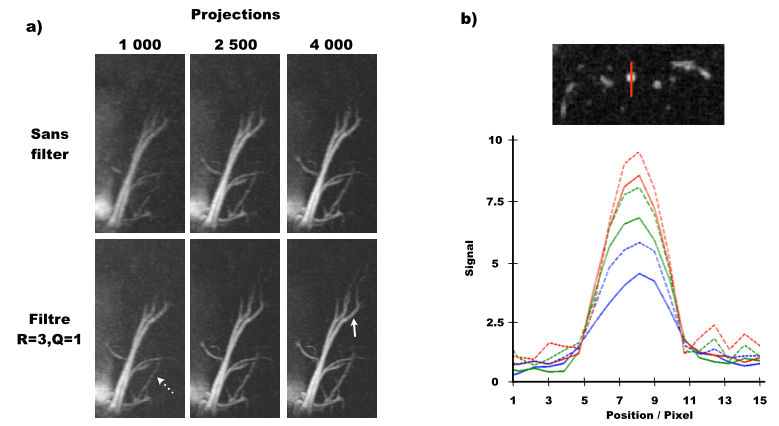
\includegraphics[scale=0.5]{./figure/chap3/ImFlowMice.png}
%\caption[Image ARM dynamique sur souris]{\label{fig:ImFlowMice} Images MIP sagital recueillies sur des carotides de souris avec la séquence dynamique. (a) Les images reconstruites avec 1000, 2500 et 4000 projections sont comparées aux images reconstruites avec l'utilisation d'un filtre temporel (R=3, Q=1). (b) Le profile d'intensité est obtenu au niveau de la ligne rouge sur les carotides après la bifurcation aortique. Lignes continues : reconstructions non-filtrées; bleu: 1000 projections; vert: 2500 projection; rouge: 4000 projections.}
%\line(1,0){400} \\ \end{figure}
%
%\begin{figure}[H]
%\centering \line(1,0){400} \\
%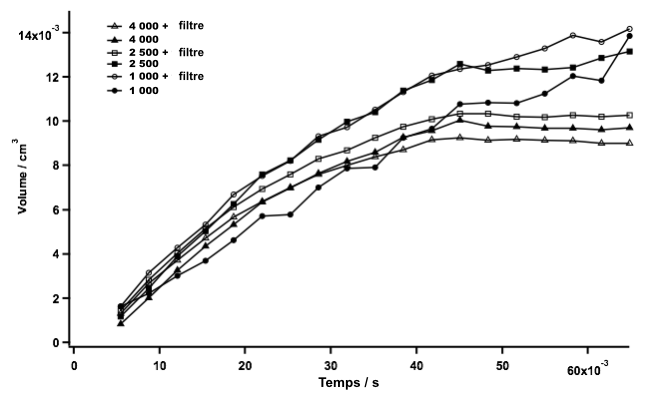
\includegraphics[scale=0.5]{./figure/chap3/GraphFlowMice.png}
%\caption[Graphique de progression du flux sur fantôme]{\label{fig:GraphFlowMice} Volume des flux mesuré en fonction du temps après l'application du module de saturation sur les carotides d'une souris saine. Les données représentées ont été recueillies avec 4000, 2500 et 1000 projections ainsi qu'avec leurs reconstruction filtrée (R=3,Q=1).}
%\line(1,0){400} \\ \end{figure}

\subsubsection{Imagerie du polygone de Willis}

%\begin{figure}[H]
%\centering \line(1,0){400} \\
%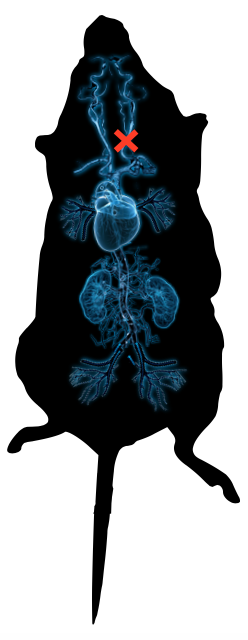
\includegraphics[scale=0.5]{./figure/chap3/LigatCarotide.png}
%\caption[Modèle de ligature des carotides]{\label{fig:LigatCarotide} Schéma du modèle de ligature de la carotide sur souris}
%\line(1,0){400} \\ \end{figure}

Des expériences ont ensuite été réalisées sur un modèle de souris normale et sur un modèle de souris présentant une ligature de la carotide commune. Des images ont été réalisées au niveau du polygône de Willis avec des résolutions spatiale et temporelle extrêmement élevées ($(156 \ \mu m)^3$ et 3,3 ms). 2500 projections ont été utilisées pour chaque image ciné et les images reconstruites avec un filtre Q=1,R=3 sont montrées dans la figure \ref{fig:ImFlowWillis}. Les images ont été synchronisées sur le cycle cardiaque de l'animal. Le temps d'acquisition total est d'environ 5 minutes (avec 500 battements cardiaques par minute).

Avec la séquence d'ARM dynamique, il a été possible d'observer chez 4 souris ayant subi une ligature de la carotide droite (figure \ref{fig:ImFlowWillis}.a) que le remplissage du polygone était compensé par le flux sanguin provenant de la carotide gauche. Cependant le délai d'arrivée du sang dans la partie droite du polygone présente un retard par rapport aux souris contrôles comme observé sur les images de la figure \ref{fig:ImFlowWillis}.b.
Ce délai a pu être quantifié sur une carte paramétrique obtenue grâce à une méthode de calcul du temps d'arrivée du sang en un point de l'espace (figure \ref{fig:ColorMapFlowWillis}).

\begin{figure}[H]
\centering \line(1,0){400} \\
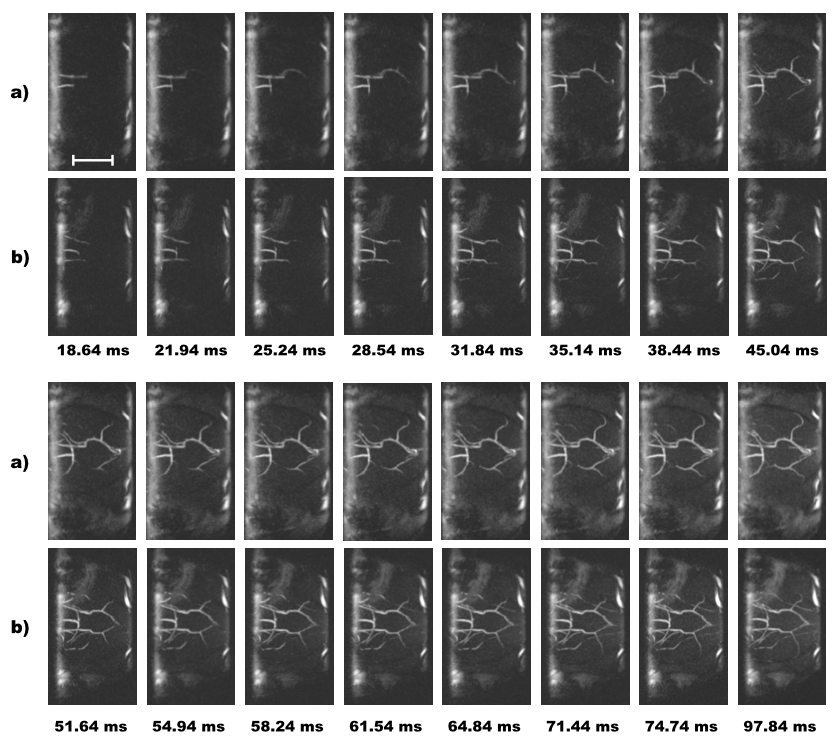
\includegraphics[scale=0.5]{./figure/chap3/ImFlowWillis.png}
\caption[Image d'ARM dynamique sur souris du polygone de Willis.]{\label{fig:ImFlowWillis} \textbf{Image d'ARM dynamique sur souris du polygone de Willis}. Image MIP d'ARM dynamique acquises sur une souris saine (a) et sur une souris ayant subi une ligature d'une artère carotide (b). 16 images ont été extraites des 30 images ciné acquises. La barre d'échelle mesure 10 mm.}
\line(1,0){400} \\ \end{figure}

\begin{figure}[H]
\centering \line(1,0){400} \\
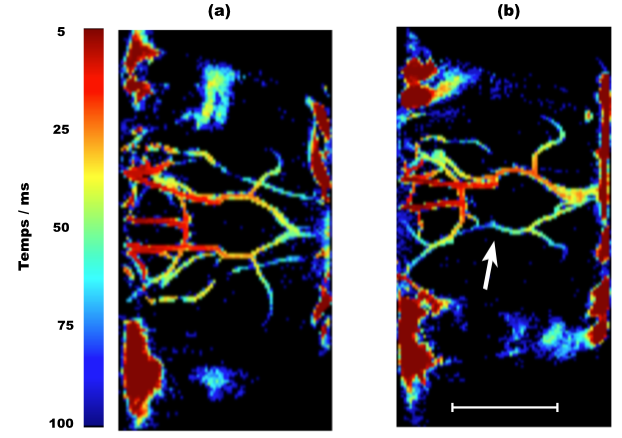
\includegraphics[scale=0.5]{./figure/chap3/ColorMapFlowWillis.png}
\caption[Quantification de la progression des flux sur une carte paramétrique.]{\label{fig:ColorMapFlowWillis} \textbf{Quantification de la progression des flux sur une carte paramétrique.} Carte paramétrique représentant le délai d'arrivée du sang dans une partie du polygone de Willis pour une souris saine (a) et pour une souris avec une artère carotide ligaturée (b). La barre d'échelle mesure 10 mm.}
\line(1,0){400} \\ \end{figure}

Il n'est pas possible d'effectuer l'imagerie sur un champ de vue plus large. En effet, le contraste vasculaire étant basé sur le principe du temps de vol, le signal sanguin sera saturé en arrivant à la fin du polygone. Une des solutions serait d'augmenter le TR de la séquence mais ceci entraînerait une moins bonne visualisation dynamique de l'avancée du flux. De plus, la différence entre deux images consécutives serait plus importante ce qui limiterait la taille du filtre temporel utilisable. Enfin un dernier problème se pose puisqu'il faudrait augmenter le nombre d'images ciné à lire après la saturation du signal ce qui induirait une repousse accrue du signal statique et donc diminuerait le contraste que l'on pourrait espérer obtenir entre le cerveaux et les vaisseaux.

L'alternative employée a été de répéter la séquence 3 fois de suite en modifiant la position de la coupe puis d'associer les images après leur reconstruction en fonction de leur position (figure \ref{fig:FluxComplet}.a). Les coupes sont disposé de manière à se superposer en partie pour limiter les effets de bord. On peut aussi reconstruire une carte paramétrique pour l'arrivée du flux mais cela demande à l'utilisateur d'indiquer à quel moment le flux d'une coupe entre dans la suivante. La figure \ref{fig:FluxComplet}.b est un exemple de représentation en carte paramétrique utilisant de multiples coupes. On observe sur ces images des artéfacts au bord des coupes qui sont dus à la mauvaise saturation du signal au bord de la sélection de coupe.

\begin{figure}[H]
\centering \line(1,0){400} \\
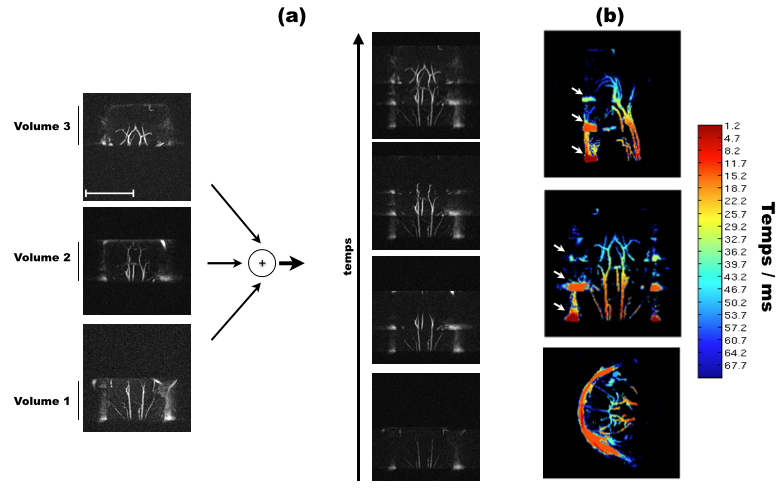
\includegraphics[scale=0.6]{./figure/chap3/FluxComplet.png}
\caption[Image d'ARM dynamique et carte paramétrique sur souris des carotides au polygone de Willis.]{\label{fig:FluxComplet} \textbf{Image d'ARM dynamique et carte paramétrique sur souris des carotides au polygone de Willis.} Imagerie des carotides jusqu'au polygone de Willis effectuée avec 3 acquisitions successives avec des coupes placées en 3 positions différentes. (a) L'association des images est effectuée après la reconstruction de chacune d'entre elles. (b) La carte paramétrique représentant l'avancée des flux doit être synchronisée pour que l'arrivée du sang dans la zone d'un premier volume débute en même temps que l'arrivée dans la même zone du volume d'imagerie suivant. La barre d'échelle mesure 10 mm.}
\line(1,0){400} \\ \end{figure}

\section{Discussion}

L'imagerie de flux chez la souris est un véritable défi du fait de la dimension des vaisseaux sanguins et des paramètres physiologiques extrêmes de la souris. Pour répondre à cette problèmatique, le développement de séquence radiale doublement pseudo-aléatoire a été préféré.

Dans un premier temps, une séquence avec une trajectoire 3D radiale projection-reconstruction pour l’ARM anatomique a été développée. Il a notamment été montré que cette méthode était beaucoup moins sensible aux artéfacts de flux et de mouvement que l’imagerie cartésienne. Ceci a permis d’obtenir des images anatomiques de la crosse aortique avec un signal très homogène malgré la respiration et les flux turbulents durant la phase systolique du coeur. Ensuite, la capacité des méthodes radiales à être sous-échantillonnée a permis d’obtenir des images ayant une qualité satisfaisante avec seulement 4000 projections. Ceci correspond à une réduction du temps d’acquisition d'un facteur supérieur à 14 par rapport au critère de Nyquist ainsi que de 10 par rapport à une séquence cartésienne standard permettant d’obtenir une imagerie avec le même champ-de-vue. 

Enfin, le troisième avantage de l’imagerie radiale mise en place ici est l’utilisation d’une trajectoire pseudo-aléatoire. Cela permet une distribution approximativement uniforme des projections au cours du temps. Cette méthode, peut être employée pour efficacement répartir les projections avec pour objectif de retirer les projections corrompues par les mouvements physiologiques. En effet, il existe des approches utilisant les points centraux des projections pour extraire des informations sur la position de celles-ci au sein de la respiration. Il peut donc être possible de reconstruire a posteriori des images à différents moments de la phase de respiration, ou bien de reconstruire des images avec les projections recueillies uniquement durant les phases de respiration avec peu de mouvement. Cette méthode de correction de mouvement n’a pas été employée ici car les acquisitions chez la souris sont peu sensibles à ce type d’artéfacts. En revanche, elle pourrait être pertinente pour une utilisation chez l’homme. Grâce à ces différents points, l’imagerie radiale utilisant une trajectoire d’angle d’or peut être particulièrement efficace pour l’imagerie anatomique temps-de-vol, en particulier si les temps d’acquisition ont besoin d’être limités ou sur des régions anatomiques sujets aux mouvements.
 

Cette approche a ensuite été étendue à l'imagerie résolue dans le temps pour visualiser la progression des flux dans les vaisseaux avec une forte résolution temporelle (3,3 ms; 300 images/seconde), une forte résolution spatiale et surtout en un temps d'acquisition réduit d'un facteur 5 par rapport à la méthode précédemment employée par Miraux et al.
L'optimisation de la séquence permet d'obtenir des temps de répétition inférieurs à 3,5 ms qui sont nécessaires pour visualiser l'avancée des flux rapides dans les artères, cela est aussi important pour permettre l'utilisation du filtre temporel qui est plus efficace lorsqu'il existe peu de différence entre les images adjacentes.
L'utilisation du filtre temporel a été rendu possible grâce à l'ajout du second angle d'or entre les trajectoires des images ciné. Celui-ci a pour effet de particulièrement bien répartir les projections entre celles-ci et permet une utilisation optimale de nombreuses formes de filtre temporel comme les filtres linéaires \cite{Barger:2002fk}, KWIC \cite{Song2004Dynamic-MRI-wit}, exponentielles etc. Cela est particulièrement important lorsque la dynamique des flux n'est pas connue ou potentiellement perturbée dans des modèles pathologiques où la résolution finale des images pourra être modulée pour obtenir des images avec une qualité adaptée à la quantification de la vitesse des flux.

\section{Limitations}

La méthode proposée présente tout de même certaines limitations :
\begin{itemize}
\item Pour obtenir un effet temps de vol efficace, il est important d’utiliser une coupe relativement fine. Ainsi, avec un encodage radial sphérique comme proposé ici, une grande partie du champ de vue est inutile. Notamment, chez l’homme, ou il est nécessaire d’utiliser des coupes très fines pour visualiser le polygone de willis (< 5 cm) le développement d’autre stratégie devra être envisagé pour utiliser l’imagerie cartésienne doublement aléatoire pour la mesure du flux sanguin. 
\item Une des difficultés de l’imagerie non-cartésienne est la nécessité de connaître parfaitement la trajectoire dans l’espace de Fourier. Il est donc nécessaire d’ajouter une preparation supplémentaire (mesure de la trajectoire) lors de l’acquisition des images. Ceci augmente le temps total d'expérience.
\item Il reste difficile de combiner reconstruction 3D non-cartésienne et méthode d’imagerie parallèle. Des publications récentes montrent que cela est possible, mais ces méthodes reste à évaluer (nuSpirit, compressed sensing, …)
\end{itemize}

\section{Perspectives}
\begin{itemize}
\item Pour le transfert de cette méthode chez l’homme, le développement des séquences de type Stack-Of-Star est envisageable. Elle permettraient en effet de limiter le champ de vue dans la direction de coupe.

\item Afin d’accélérer encore la méthode proposée, une collaboration avec C Mistretta a débuté pour tester les méthodes de reconstruction de type HYPR (HighlY constrained back-PRojection). Ces dernières semblent particulièrement bien adaptée à notre stratégie qui génèrent un signal de fond très faible.
\end{itemize}

%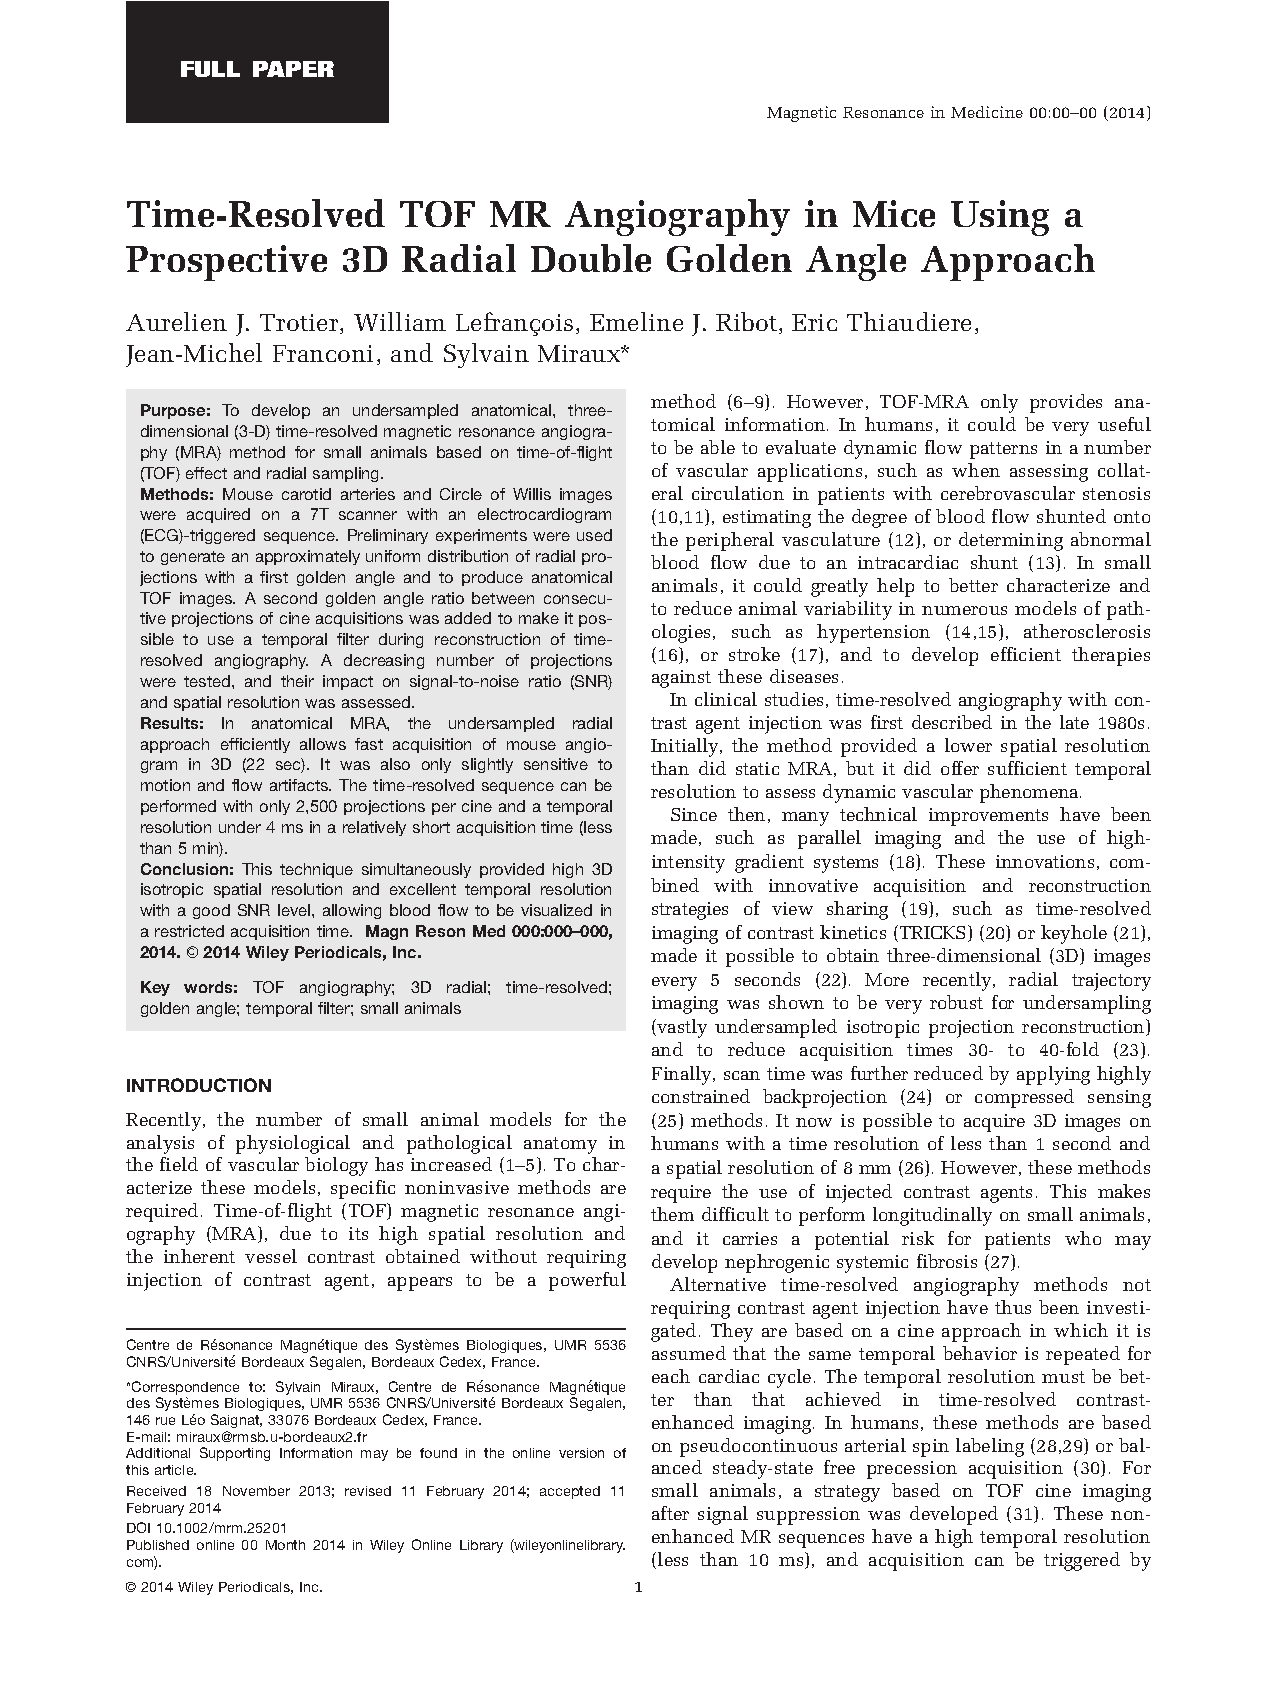
\includepdf[pages=1-11]{./figure/chap3/Papier1.pdf}
%
\chapter{Développement d'une méthode d'imagerie cardio-vaculaire sang blanc 3D associant une séquence à temps d'écho ultracourt à l'injection d'un agent de contraste à base de nanoparticule de fer.}
\setlength{\footskip}{50pt}
\chaptermark{Angiographie cardiaque UTE}
\label{Chap4}
\section{Contexte}


L’IRM est devenue un outil de référence pour l’imagerie cardiovasculaire car elle peut permettre d’obtenir de manière non-invasive des informations anatomiques mais aussi fonctionnelles du coeur. L’imagerie cardiaque résolue dans le temps (appelée imagerie ciné) s’est donc fortement développée que ce soit chez l’homme ou le petit animal. 
Aujourd'hui les examens de routine sont réalisés en imagerie sang blanc 2D, multi-coupes. Cependant, ce type d'acquisition ne permet pas d’obtenir une résolution importante dans la direction de coupe. Elles peuvent sous-estimer des défauts de contraction du myocarde ou donner des informations sur la fraction d’éjection peu précises, en particulier pour des cas pathologiques entraînant des modifications de la paroi du myocarde \cite{Friedrich:2000aa}. De plus, elles nécessitent un positionnement précis des coupes d'imagerie qui peut s'avérer complexe, notamment chez le petit animal.

Le passage à l'imagerie 3D-t pour des applications cardiovasculaires a donc un intérêt considérable. Cependant, celle-ci est confrontée au faible contraste-sur-bruit entre le sang et le myocarde induit par la saturation du signal sanguin à l'intérieur des cavités cardiaques inhérente à l'utilisation des séquences traditionnelles d'imagerie cardiaque de type écho de gradient. 
De nouvelles stratégies ont été employées pour obtenir de meilleurs rapports signal-sur-bruit et contraste-sur-bruit. Celles-ci se basent sur l’utilisation des séquences de type “Balanced Steady-State Free Precession” (bSSFP) qui permettent d’obtenir un meilleur signal des liquides et donc du sang \cite{Nezafat2008Inflow-quantifi}. Cependant cette méthode est sensible aux variations locales de champ magnétique ce qui a pour effet de créer des artefacts caractéristiques sous forme de bandes noires dans les images. Plus le volume à imager est important, comme c’est le cas en 3D, plus le nombre de bandes noires est important. Cela explique la faible utilisation de ces séquences à des champs magnétiques intenses et en particulier sur le petit animal. Des méthodes de correction de ces artefacts ont été développées \cite{Bangerter:2004kq} et appliquées à hauts champs magnétiques pour l’imagerie cardiaque \cite{Miraux:2008sf}.  Cependant, ce type de méthode requiert un temps d’acquisition quatre fois plus important \cite{Miraux:2008sf}. 
Une autre approche possible est l'utilisation de séquences sang noir qui permettent d'obtenir des mesures plus précises de l'anatomie cardiaque \cite{Berr2005Black-blood-gra}. En effet, les images sang noir ne sont pas sensibles aux artefacts de déphasage de flux qui provoquent des incertitudes sur les mesures anatomiques en particulier durant la phase systolique. Néanmoins, cela se fait au détriment du rapport signal-sur-bruit, et nécessite par ailleurs d’augmenter le temps d’acquisition des images  \cite{Miraux:2009rm}.

En pratique clinique, l’injection d’agents de contraste à base de gadolinium peut être utilisée pour l’imagerie cardiaque résolue dans le temps. En revanche, cette stratégie n’est pas adaptée pour des applications précliniques. En effet le gadolinium, de par son faible poids moléculaire, diffuse facilement dans le compartiment interstitiel ce qui a pour effet de rehausser le signal dans le myocarde et donc de diminuer le contraste avec le sang.

L’utilisation d’agents de contraste à base de nanoparticules de fer (Ultra Small Particle of Iron Oxyde : USPIO) en tant qu’agent de contraste positif restreint au système vasculaire semble être une bonne alternative aux agents à base de gadolinium grâce à leurs temps de demi-vie dans le sang relativement élevés  \cite{Corot:2006fk,Neuwelt:2009aa}. Il a déjà été montré que ce type d’agent de contraste pouvait être utilisé en tant qu’agent de contraste $T_1$ à des champs magnétiques cliniques (1,5T et 3T) pour l’imagerie de premier passage \cite{Li:2005uq}, pour l'imagerie vasculaire \cite{Sigovan:2009aa,Nayak:2014aa} ainsi que pour l'imagerie cardiaque \cite{Amano:2000aa}.

Cependant la plupart des IRM précliniques disponibles utilisent des champs magnétiques supérieurs ou égaux à 4,7T. Hors, à hauts champs magnétiques, l'effet $T_2^*$ provoqué par les USPIOs est important alors que l'effet $T_1$ est pratiquement stable. Cela explique pourquoi les USPIOs sont principalement utilisés en tant qu'agents de contraste négatif chez la souris, hormis quelques travaux \cite{Jung:2014aa,Girard:2011ec,Loubeyre:1997aa} mais ceux-ci sont réalisés à 3T.

Afin de générer un contraste positif à hauts champs magnétiques, différentes stratégies ont été mises en oeuvre (Saturation Off-Résonance (ORS), l'imagerie de susceptibilité ou des méthodes de compensation de gradient). Toutes ces méthodes ont la même limitation, elles utilisent les perturbations du champ magnétique provoquées par les USPIOs. Or, celles-ci ne peuvent être différenciées d'autres sources de perturbation (interface air/tissus, imperfection du champ $B_0$, etc) qui sont plus présentes à hauts champs magnétiques et rendent donc leurs applications difficiles dans des études précliniques.

L'alternatives la plus efficace pour limiter la décroissance du signal provoquée par les agents de contraste à base de nanoparticules de fer est de réduire fortement le temps d'écho des séquence. L'utilisation de séquences à temps d'écho ultracourts (UTE) permet de s'affranchir de l'effet $T_2$ et $T_2*$ des tissus \cite{Tyler2007Magnetic-resona} et d'utiliser efficacement l'effet $T_1$ des USPIOs. Cette approche est prometteuse pour des applications \textit{in vivo} en particulier dans le champ de l'imagerie quantitative \cite{Girard:2011ec,Gharagouzloo2015Quantitative-co}.


Dans ce chapitre, nous montrerons qu'en combinant l'utilisation d'une séquence 3D UTE (TE < 0.050 ms) et l'injection d'USPIO il est possible d'obtenir un contraste positif quelle que soit la valeur du champ  magnétique (4,7T, 7T et 9,4T) ainsi qu'avec une large gamme de concentrations d'USPIO injectés. A partir de ce principe nous montrerons qu’il est possible, grâce à un schéma d’acquisition original d’obtenir, à partir d’un même jeu de données acquis, des images 3D+temps de tout le système cardiovasculaire soit avec une forte résolution spatiale, soit une forte résolution temporelle.


\section{Angiographie rehaussée par un agent de contraste à base de nanoparticules de fer}

\subsection{Agent de contraste}

Les agents de contraste à base de particules de fer sont séparés en plusieurs catégories en fonction de leurs tailles. Les USPIOs ont une taille inférieure à 50 nm. Ils sont composés d’un noyau cristallin d’oxyde de fer entouré d’un “coating” (enrobage généralement composé de dextran) qui évite leur agrégation dans l’organisme. Les USPIOs sont généralement captés par le foie et la rate après une injection par voie intraveineuse. Une des propriétés qui est intéressante pour l'imagerie cardiaque est leur longue durée de demi-vie plasmatique (de 24 à 36 heures chez l'humain et d'environ 2 heures chez la souris).

Durant ce projet, plusieurs type d'USPIOs ont été utilisés : 
\begin{enumerate}
\item Le Sinerem \textregistered \ (Guerbet, France) : il s'agit d'un dérivé du ferumoxtran-10 possédant un petit diamètre hémodynamique (30 nm) et un long temps de rémanence vasculaire. Celui-ci est extrêmement espèce dépendant (Demi-vie plasmatique de 36 heures chez l'homme, de 6 heure chez le lapin, de 2 heures chez le rat). Le ferumoxtran-10 est complètement dégradé dans les lyposomes des macrophages en sept jours. Celui-ci a été autorisé sur le marché européen pour la détection des métastases des ganglions lymphatiques.

\item Le P904 (Guerbet, France) : il s'agit un agent de contraste prototype préclinique mis en place pour l'imagerie des macrophages, l'imagerie cellulaire ou l'angiographie. Sa demi-vie plasmatique est également espèce dépendante (Chez la souris : 60 minutes, chez le rat : 145 minutes).
\end{enumerate}

\subsection{Relaxivités}

Les relaxivités $r_1$ et $r_2$ de ces deux agents de contraste évoluent de façon équivalente en fonction du champ magnétique. Avec l'augmentation de celui-ci, la valeur de $r_1$ reste quasi-constant et la valeur de $r_2$ va augmenter fortement. Les valeurs de $r_1$ et $r_2$ mesurées pour le Sinerem dans une solution saline sont respectivement de $1,14 \pm 0,06 \ mM^{-1}.sec^{-1}$ et $36,46 \pm 3,03 \ mM^{-1}.sec^{-1}$ à 4,7T; $1,13 \pm 0,09 \ mM^{-1}.sec^{-1}$ et $65,21 \pm 4,23 \ mM^{-1}.sec^{-1}$ à 7T; $1,14 \pm 0,1 \ mM^{-1}.sec^{-1}$ et $86,23 \pm 3,81 \ mM^{-1}.sec^{-1}$ à 9,4T

Les résultats présentés dans la suite du chapitre ont été obtenus avec l'injection du Sinerem mais des résultats équivalents ont aussi été obtenus avec le P904 sa relaxivité étant proche de celle du Sinerem.

\subsection{Contraste positif en fonction du champ magnétique et de la concentration}

Pour évaluer l'effet de l'agent de contraste sur les images, une séquence 3D UTE (TE = 0,031 ms) a été utilisée sur des souris injectées avec 3 valeurs de concentrations de Sinerem (100, 200 et 500 $\mu$mol de fer/kg) pour obtenir des images sur une zone allant du foie au cou ainsi que sur des souris avant injection. Ces valeurs de concentrations ont été choisies car elles correspondent à une gamme de concentration allant des valeurs utilisées pour l'injection chez l'humain aux valeurs de concentration utilisées pour le ciblage cellulaire.
Les paramètres des séquences ont été fixés pour obtenir une résolution de $(234 \ \mu m)^3$ isotropique et pour un temps d'acquisition de 3 min 51 sec.

Des images, sans synchronisation cardiaque ni respiratoire, pré et post-injection obtenues à 9,4 T sont montrées dans la figure \ref{fig:UTEConcen}.  Avant l'injection de l'agent de contraste, les vaisseaux sanguins et le sang dans les cavités du coeur ne sont pas facilement identifiables par rapport aux tissus adjacents.

\begin{figure}[H]
\centering
\line(1,0){400} \\
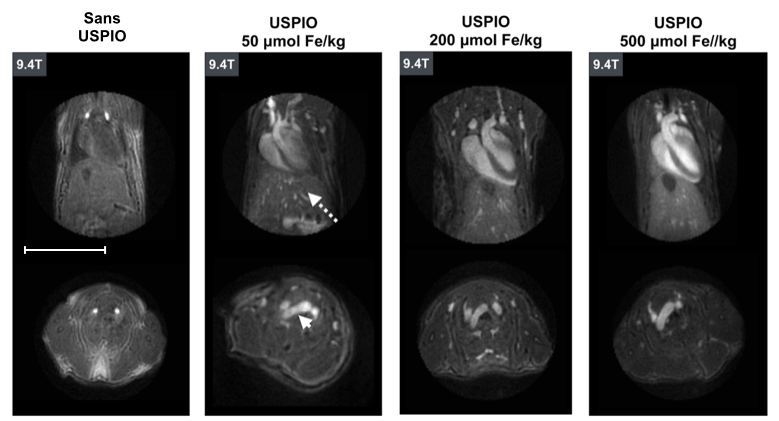
\includegraphics[scale=0.55]{./figure/chap4/Fig_2.png}
\caption[Images obtenues avec une séquence UTE en fonction de la concentration d'USPIO injectés.]{\label{fig:UTEConcen} \textbf{Images obtenues avec une séquence UTE en fonction de la concentration d'USPIO injecté.} Images obtenues sur le coeur et le foie de souris avec une séquence 3D UTE à 9,4T. Les images ont été obtenues avant et après injection d'agents de contraste à différentes concentrations (100, 200 et 500 $\mu$mol Fe/kg), sans synchronisation cardiaque ou respiratoire. La barre d'échelle représente 15 mm.}
\line(1,0){400} \\ 
\end{figure}

Après l'injection de l'agent de contraste, le sang dans les vaisseaux est visible avec la séquence UTE avec un signal intense et ce, quelle que soit la dose injectée. Ce signal est très homogène même dans les zones avec de fortes turbulences comme la crosse aortique indiquée par la flèche blanche ou dans les vaisseaux avec un faible débit comme les veines jugulaires. Peu d'artefacts de flux ou de mouvement sont observés ce qui s'explique par la trajectoire radiale (voir la section \ref{subsec:MouvEtFlux}) ainsi que par le faible TE et l'absence de déphasage des spins par les gradients avant la lecture du signal.

Des observations similaires ont été faites à 4,7 et 7T. Des valeurs de contraste-sur-bruit ont été mesurées entre le sang (dans la crosse aortique et les veines jugulaires) et les muscles et sont répertoriées dans la figure \ref{fig:contraste-sur-bruitUteFlash}. On observe avec la séquence UTE un contraste-sur-bruit d'environ -2 avant injection et une augmentation importante de celui-ci après injection permettant d'obtenir des valeurs toujours supérieures à 18. Cette augmentation est fonction de la dose injectée et la plus forte concentration permet d'obtenir un contraste-sur-bruit supérieur à 40. Cette observation s'explique par le fait que la séquence UTE est peu impactée par l'augmentation du $T_2^*$ grâce à son TE ultracourt, au contraire son signal augmente grâce à l'effet $T_1$ des USPIOs.
Le deuxième point à noter est que le signal diminue aussi avec l'augmentation du champ magnétique pour chaque concentration, cela peut s'expliquer par l'augmentation des valeurs de relaxivité $r_2*$. Cependant cette diminution est très faible et n'est pas significative sur nos mesures.

\begin{figure}[H]
\centering
\line(1,0){400} \\
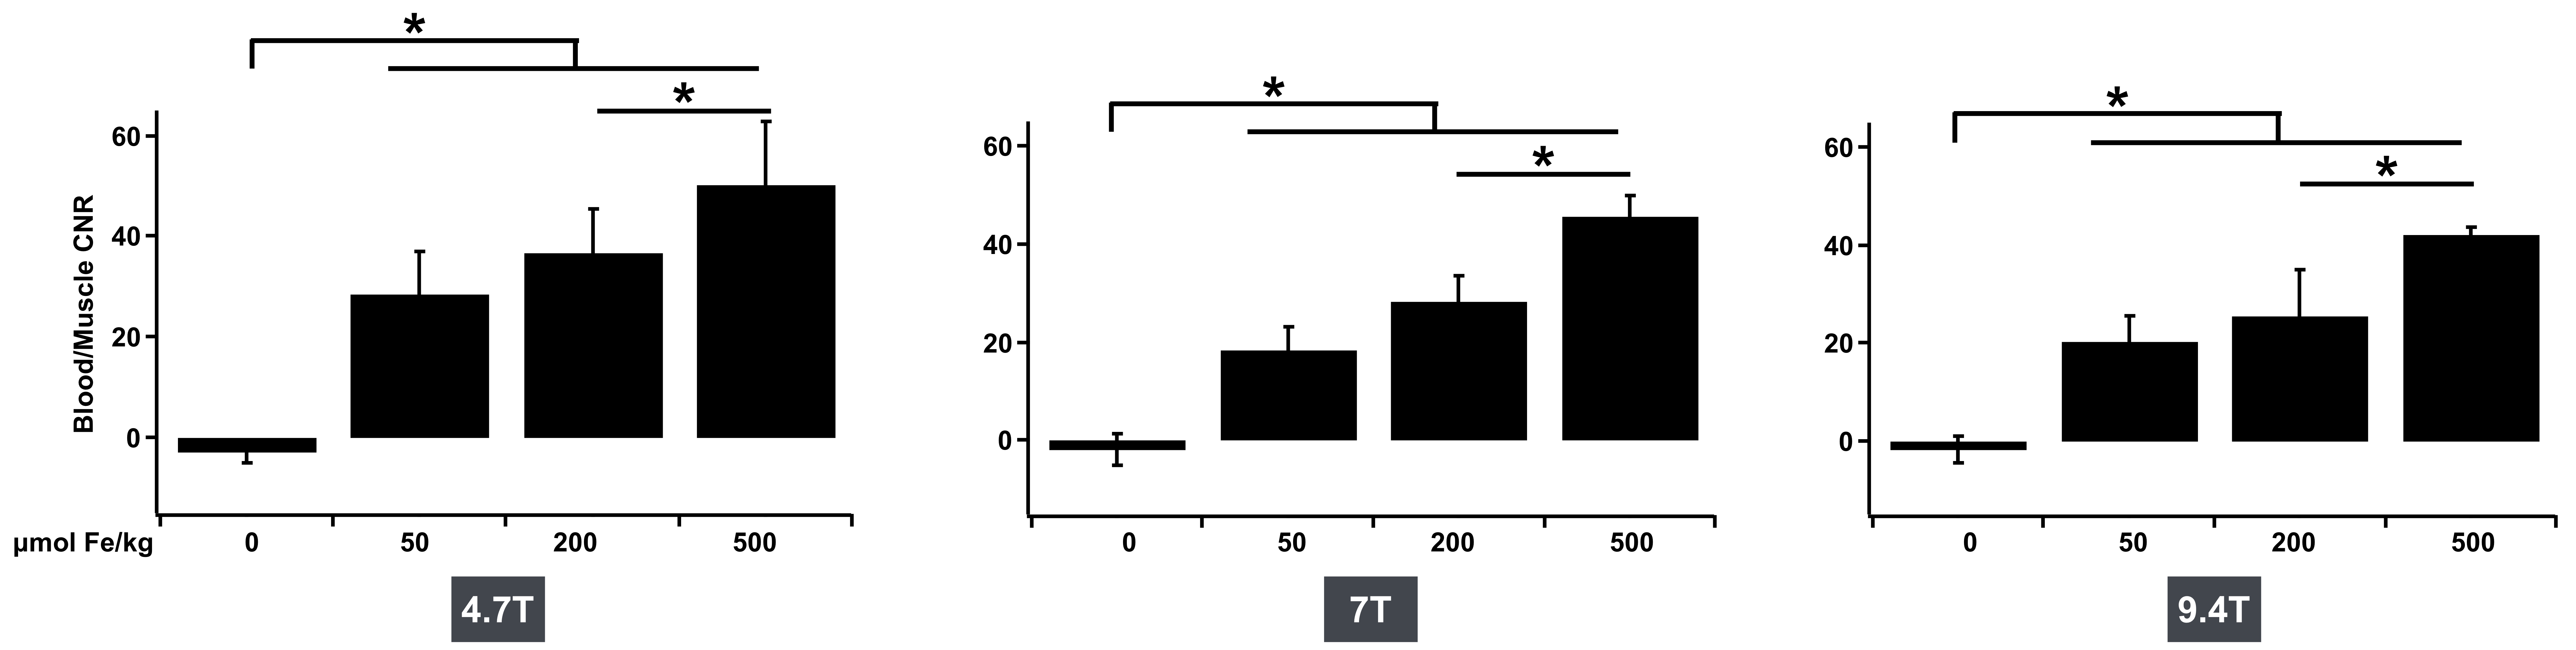
\includegraphics[scale=0.22]{./figure/chap4/Fig_3.png}
\caption[Quantification du rapport contraste-sur-bruit.]{\label{fig:contraste-sur-bruitUteFlash} \textbf{Quantification du rapport contraste-sur-bruit.} Mesure du rapport contraste-sur-bruit entre la crosse aortique et le muscle obtenu avec une séquence UTE avant et après injection d'USPIO à 4,7 T, 7 T et 9,4 T et pour différentes concentrations injectées (100, 200 et 500 $\mu$mol Fe/kg). Les valeurs de p inférieures à 0,05 sont indiquées par des astérisques.}
\line(1,0){400} \\ 
\end{figure}

Il est à noter que pour la plus faible concentration de Sinerem injectée (50 $\mu$mol Fe/kg), le contraste varie au cours des expériences : celui-ci a tendance à diminuer d'environ 30 $\%$ au bout d'une heure. Au contraire, les mesures de contraste-sur-bruit restent stables pendant cette période avec les deux concentrations supérieures. 

Tous ces points font de la méthode d'imagerie combinant l'injection d'USPIO et l'utilisation d'une séquence UTE une stratégie envisageable pour l'angiographie 3D et en particulier l'imagerie cardiaque.

\section{Angiographie cardiaque 3D résolue dans le temps}

Au vu du très bon signal obtenu sur les images précédentes, il a donc été envisageable de développer une séquence 3D résolue dans le temps. Cependant l'application de la méthode ciné à la séquence UTE nécessite trop de temps d'acquisition si l'on souhaite obtenir des images respectant le critère de Nyquist. Par exemple, pour des images avec une matrice $(128)^3$, il serait nécessaire de recueillir 102943 projections (qui sont des rayons dans le cas des séquences UTE) ce qui correspondrait à un temps d'acquisition de 257 minutes chez une souris anesthésiée avec un rythme cardiaque à 450 battements par minute. Il est possible de sous-échantillonner l'acquisition d'un facteur 2 en impactant peu la résolution mais cela n'apparaît pas suffisant.
Un des avantages des séquences UTE est qu'elles possèdent un faible TR. Il est donc possible de recueillir de nombreux signaux IRM (au moins 40) entre deux battements de coeur. Des signaux peuvent être regroupés pour diminuer le temps d'acquisition mais en limitant le nombre d'images résolues dans le temps qui seront reconstruites. 
Cependant, cette méthode nécessite de modifier la séquence pour que les signaux recueillis successivement ne suivent pas les mêmes trajectoires.


\subsection{Séquence}

Une séquence UTE a donc été développée permettant d'obtenir un nombre d'images ciné (NCine) dont un nombre de signaux IRM recueillis successivement, noté NRegroup, seront regroupés pour reconstruire une image ciné. Dans les expériences chez la souris les paramètres ont généralement été fixés à NCine = 10 et NRegroup = 4. Cela correspond donc à une acquisition de $10 \times 4 = 40$ signaux de décroissance de précession libre (FIDs) à recueillir entre deux battements. Ces paramètres peuvent être adaptés en fonction du rythme cardiaque de l'animal ainsi que du TR de la séquence. Par exemple, avec des TRs de 2 ms pour une souris présentant un intervalle de 140 ms entre deux ondes R de l'ECG, il est donc théoriquement possible de recueillir 70 signaux et de les regrouper par groupe de 7 pour reconstruire 10 images ciné et accélérer la séquence d'un facteur 7.

La séquence développée est présentée dans la figure \ref{fig:SeqUTEUSPIO} avec pour paramètres NCine = 10 et NRegroup = 4. Les différentes projections radiales sont acquises en partant d'une première projection verticale orientée selon z puis s'écartent progressivement de z en tournant autour de ce dernier décrivant ainsi une spirale sur le pourtour de l'espace de Fourier (sphérique) \cite{Saff1997}.
 La position des projections est définie par :
%La trajectoire utilisée pour positionner les projections est une spirale qui part en haut de l'axe Z et termine en bas en tournant autour de l'axe \cite{Saff1997}.
\begin{equation}
\begin{split}
	& Pour \ 1 \leq k \leq NPro : \\ 
	& h_k = -1+\frac{2(k-1)}{NPro-1} \\
	& \Theta_k = arcos(h_k) \\
	& \\
	& \Phi_1=\Phi_N=0 \\	
	& pour \ 2 \leq k \leq N-1 \\
	& \Phi_k=\left( \Phi_{k-1}+\frac{3,6}{\sqrt{NPro\times (1-h_k^2)}} \right)mod(2 \pi)	
\end{split}
\end{equation}
où NPro correspond au nombre de projections choisi pour parcourir un espace de Fourier complet. La méthode de répartition des trajectoires permet de les répartir de manière uniforme dans une sphère et ce quel que soit le nombre NPro défini. Cependant dans le cadre de cette séquence, NPro doit être un multiple de NRegroup pour regrouper les projections ensembles afin de former une image.

\begin{figure}[H]
\centering
\line(1,0){400} \\
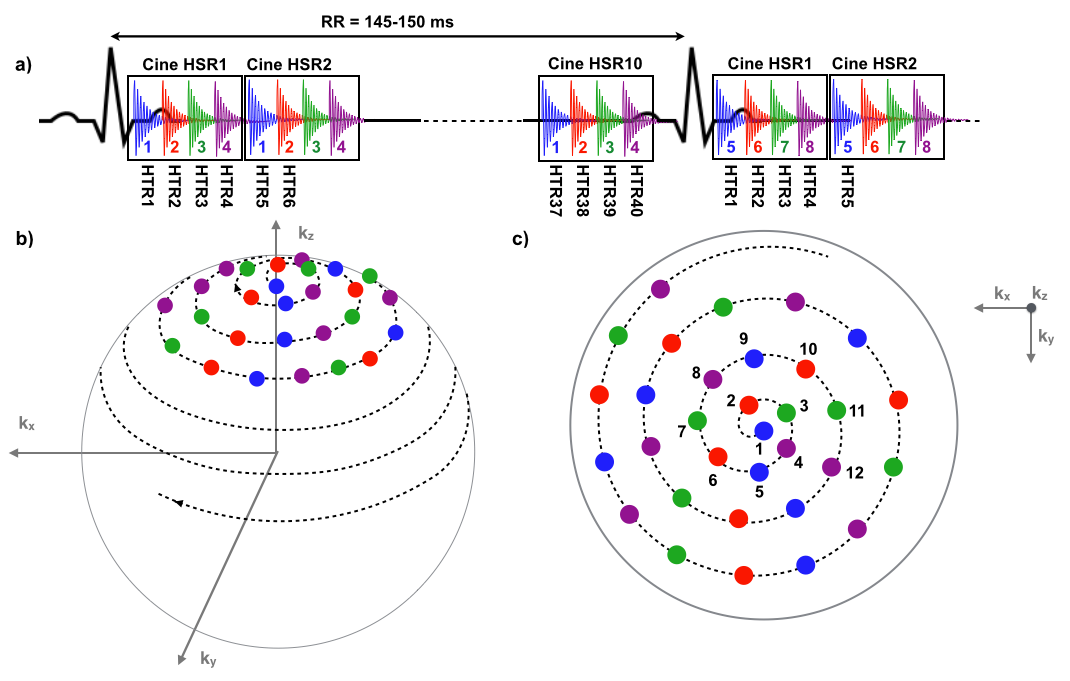
\includegraphics[scale=0.5]{./figure/chap4/SeqUTEUSPIO.png}
\caption[Schéma d'acquisition de la séquence 3D UTE synchronisée sur le rythme cardiaque.]{\label{fig:SeqUTEUSPIO} \textbf{Schéma d'acquisition de la séquence 3D UTE synchronisée sur le rythme cardiaque.} La séquence est représentée avec NCine = 10 et NRegroup = 4. a) Représentation des projections recueillies selon une trajectoire indiquée par le nombre en couleur et servant à remplir des espaces de Fourier indiqués par le terme HTR ou HSR. Les espaces de Fourier HSR correspondent à une reconstruction avec une forte résolution spatiale alors que les espaces de Fourier HTR correspondent à une reconstruction avec une forte résolution temporelle. Les trajectoires sont représentées sur des espaces de Fourier en vue 3D (b) et une vue selon l'axe $k_x - k_y$ (c).}
\line(1,0){400} \\ 
\end{figure}

Les NRegroup = 4 premières projections sont recueillies selon des trajectoires différentes  avec dans l'ordre les (n$\degres$ 1, 2, 3 et 4) comme montré sur la figure \ref{fig:SeqUTEUSPIO}.c. Ce schéma d'acquisition de trajectoires est répété NCine = 10 fois jusqu'au prochain battement de coeur où les 4 trajectoires suivantes (n$\degres$ 5, 6, 7 et 8) sont alors acquises, NCiné fois, avant de passer aux suivantes, etc.

\subsection{Reconstruction}

\begin{figure}[H]
\centering
\line(1,0){400} \\
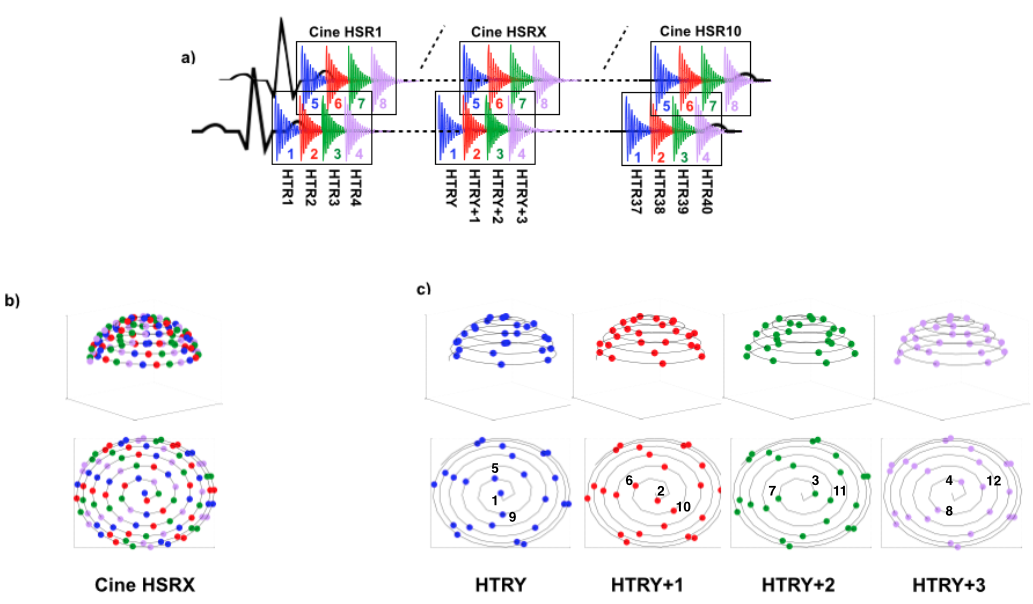
\includegraphics[scale=0.48]{./figure/chap4/RecoUTEUSPIO.png}
\caption[Combinaison et reconstruction des données.]{\label{fig:RecoUTEUSPIO} \textbf{Combinaison et reconstruction des données.} Représentation des projections utilisées pour reconstruire les jeux de données a) haute résolution spatiale et b) haute résolution temporelle.}
\line(1,0){400} \\ 
\end{figure}

Ce schéma d'acquisition permet de reconstruire à partir d'un même jeu de données acquis deux types d'images : NCine images avec une forte résolution spatiale (HSR : High Spatial Resolution) ou NCine $\times$ NRegroup images avec une forte résolution temporelle (HTR : High Temporal Resolution). Pour reconstruire les images avec la forte résolution spatiale il faut utiliser toutes les projections recueillies durant la phase Cine HSRX (1245-5678-...) comme indiqué sur la figure \ref{fig:RecoUTEUSPIO}.a et b. L'espace de Fourier reconstruit est donc échantillonné avec NPro projections.
Pour les images avec une forte résolution temporelle, il faut séparer les projections recueillies dans chaque cine HSRX en 4 sous-parties correspondant aux couleurs des projections (voir figure \ref{fig:RecoUTEUSPIO}.a et c) que l'on reconstruira pour obtenir des images avec une résolution temporelle plus importante (NRegroup fois plus grande). Les images reconstruites auront donc une plus faible résolution spatiale car le nombre de projections utilisées par images ciné sera NRegroup fois plus faible mais les projections seront réparties de manière pratiquement uniforme grâce à la trajectoire utilisée.

\subsection{Imagerie cardiovasculaire résolue dans le temps}

\subsubsection{Acquisitions à 4,7T, 7T et 9,4T}

Des images 3D résolues dans le temps ont été recueillies avec une résolution de 156 $\mu$m isotrope pour les 3 champs magnétiques disponibles. La concentration intermédiaire de 200 $\mu$mol de Fe/kg a été injectée pour obtenir les images de la figure \ref{fig:UTEUSPIOField} mais des résultats similaires ont été observés avec la plus forte concentration. Ces images ont été obtenues avec pour paramètres : NCine = 10; NRegroup = 4; NPro = 18144; ce qui correspond à un temps d'acquisition d'environ 12 minutes.

\begin{figure}[H]
\centering
\line(1,0){400} \\
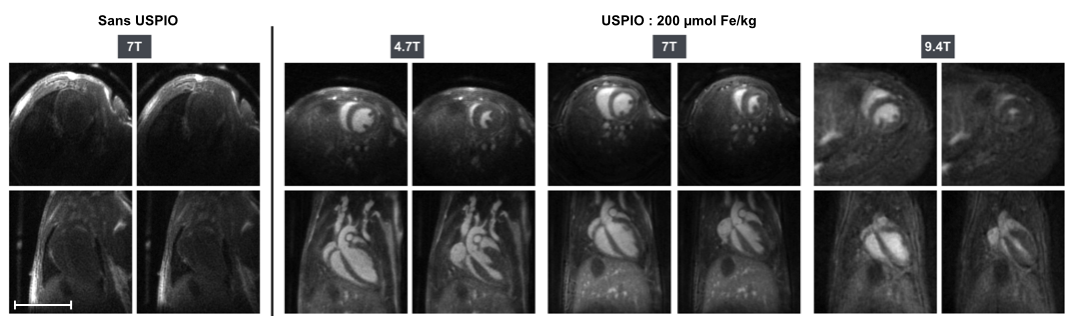
\includegraphics[scale=0.4]{./figure/chap4/Fig_4.png}
\caption[Images résolues dans le temps à plusieurs champs magnétiques.]{\label{fig:UTEUSPIOField} \textbf{Images résolues dans le temps à plusieurs champs magnétiques.} Images 3D obtenues sur un coeur de souris avec une résolution de 156 $\mu$m isotrope à différents champs magnétiques avant et après l'injection d'USPIO à 200 $\mu$mol de Fe/kg. 10 images ont été reconstruites par cycle cardiaque, des images à la fin de la diastole (gauche) et de systole (droite) sont montrées dans deux orientations (En haut : petit axe; en bas : grand axe).}
\line(1,0){400} \\ 
\end{figure}

Des mesures de signal-sur-bruit et contraste-sur-bruit ont été effectuées dans le sang et le myocarde. Le contraste-sur-bruit obtenu avant injection est d'environ -3. Après injection et quel que soit le champ magnétique, un contraste positif est obtenu entre le sang et la paroi du myocarde tout au long du cycle cardiaque (voir les mesures figure \ref{fig:TableMidRes}). Le signal obtenu est très homogène dans les vaisseaux sanguins mais aussi dans les cavités du coeur : le signal mesuré sur les expériences à 7T montre que la déviation standard du signal-sur-bruit mesuré dans le sang des ventricules et la crosse aortique a une valeur comprise entre 1,42 et 2,2 pour un signal-sur-bruit de 70. La qualité des images obtenues à 4,7T et 7T est équivalente. Par contre à 9,4T les mesures de signal-sur-bruit/contraste-sur-bruit sont plus faibles ce qui s'explique par l'utilisation d'une antenne volumique de moins bonne qualité que les antennes surfaciques à 4 éléments utilisées à 4,7 et 7T.

\begin{figure}[H]
\centering
\line(1,0){400} \\
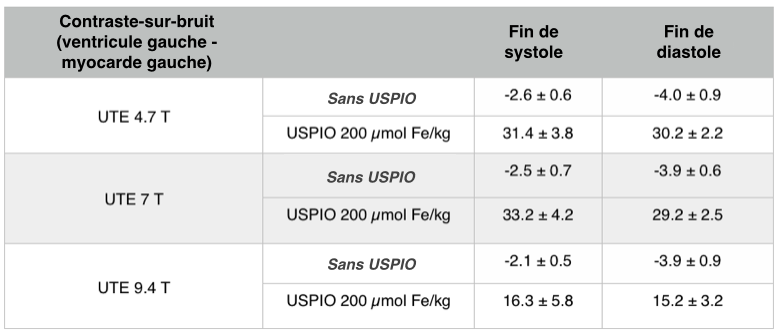
\includegraphics[scale=0.5]{./figure/chap4/TableMidRes.png}
\caption[Tableau des mesures de contraste-sur-bruit.]{\label{fig:TableMidRes} \textbf{Tableau des mesures de contraste-sur-bruit.} Mesures du contraste-sur-bruit entre le sang dans les ventricules et la paroi du myocarde sur des images obtenues avec la séquence UTE avec une résolution de 156 $\mu$m isotrope à différents champs magnétiques avant et après l'injection d'USPIO à 200 $\mu$mol de Fe/kg.}
\line(1,0){400} \\ 
\end{figure}

\subsubsection{Acquisitions haute résolution spatiale et temporelle.}

Des images ont été acquises avec une forte résolution (104 $\mu$m isotrope) à 7T (figure \ref{fig:UTEUSPIOHRS}). Ces images ont été obtenues avec pour paramètres : NCine = 10; NRegroup = 4; NPro = 52540; ce qui correspond à un temps d'acquisition d'environ 35 minutes.
La concentration de l'agent de contraste injecté (200 $\mu$mol de Fe/kg) permet d'obtenir un très bon rapport signal-sur-bruit dans le sang (40,2 $\pm$ 2,3) et un bon contraste-sur-bruit entre le sang et le myocarde (15,8 $\pm$ 2,0) durant la durée de l'expérience.
Cette forte résolution nous permet d'obtenir des mesures de volumétrie précises qui sont en accord avec celles décrites dans la littérature. De plus, elle permet de parfaitement visualiser la déformation de la crosse aortique au cours du cycle cardiaque, de distinguer les valves aortiques (Petite flèche, figure \ref{fig:UTEUSPIOHRS}.a) et de suivre le mouvement des artères coronaires droite et gauche (flèches figure \ref{fig:UTEUSPIOHRS}.b).

\begin{figure}[H]
\centering
\line(1,0){400} \\
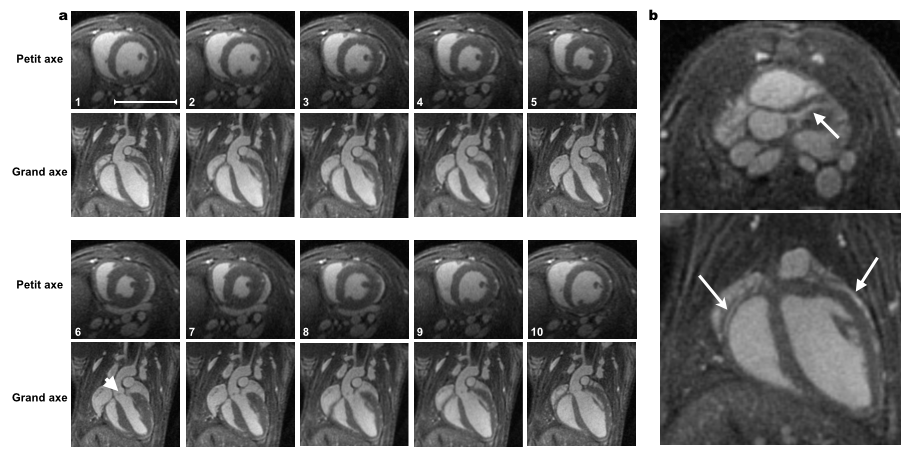
\includegraphics[scale=0.5]{./figure/chap4/UTEUSPIOHRS.png}
\caption[Images haute résolution spatiale.]{\label{fig:UTEUSPIOHRS} \textbf{Images haute résolution spatiale.} a) Images 3D résolues dans le temps au cours du cycle cardiaque (1 image/14 ms), obtenues à 7T avec une résolution isotrope de 104 $\mu$m après l'injection d'USPIO à 200 $\mu$mol de Fe/kg. Le petit axe est représenté dans la rangée du haut et le grand axe dans la rangée du dessous. La flèche (image 6) indique la valve aortique. b) Images extraites du volume 3D permettant de visualiser les artères coronaires. La barre d'échelle correspond à 1 cm.}
\line(1,0){400} \\ 
\end{figure}

A partir du même jeu de données il est aussi possible de reconstruire des images avec une forte résolution temporelle (figure \ref{fig:UTEUSPIOHRT}). Celles-ci permettent de visualiser la déformation du myocarde au cours du cycle cardiaque ce qui peut permettre d'étudier des modèles de trouble de la conduction qui induiront un délai dans la contraction. 

Les vidéos des différentes images obtenues sont disponibles sur \url{http://www.jcmr-online.com/content/17/1/53/additional}.

\begin{figure}[H]
\centering
\line(1,0){400} \\
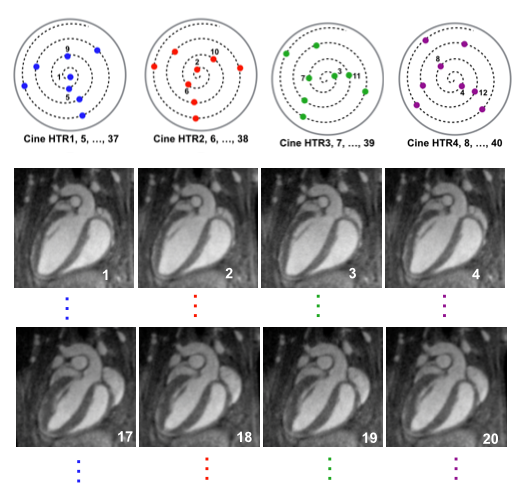
\includegraphics[scale=0.5]{./figure/chap4/UTEUSPIOHRT.png}
\caption[Images haute résolution temporelle.]{\label{fig:UTEUSPIOHRT} \textbf{Images haute résolution temporelle.} Images 3D résolues dans le temps avec une forte résolution temporelle de 3,5 ms.}
\line(1,0){400} \\ 
\end{figure}

\section{Discussion}

Malgré ses nombreux avantages en terme de résolution spatiale, l’imagerie 3D n’est pas la méthode de référence pour étudier le coeur chez le petit animal. En effet, la principale limitation est le temps d’acquisition élevé pour générer ces images, lié à un contraste faible entre le sang et le myocarde. Dans cette optique, une nouvelle méthode d’imagerie cardiaque a été proposée au cours de cette thèse. Elle permet d’obtenir un rapport signal-sur-bruit important ainsi qu’un contraste élevé entre le sang et le myocarde. Ainsi, des images avec des résolutions spatiale et temporelle inégalées ont pu être générées dans un temps d’acquisition de l’ordre de 30 minutes. Le contraste et les résolutions obtenus grâce à cette stratégie sont supérieurs à ceux qui sont décrits dans la litérature en imagerie 4D chez la souris que ce soit en : temps-de-vol \cite{Feintuch:2007aa}, avec l'injection de liposomes remplis de gadolinium \cite{Bucholz:2008uq,Bucholz:2010aa} ou par imagerie sang noir \cite{Miraux:2009rm}.

Pour obtenir un contraste sang blanc en imagerie 3D, le choix s'est porté vers l'utilisation d'agents de contraste à base de nanoparticules de fer. Ils permettent grâce à leur effet $T_1$ de rehausser le signal du sang et grâce à leur longue rémanence vasculaire de générer cet effet pendant une période supérieure à 1 heure. Une alternative possible est l'utilisation d'agents de contraste restreints au domaine vasculaire comme des liposomes chargés au gadolinium \cite{Ersoy:2004aa} mais ces agents n'ont pour le moment pas été approuvés pour des utilisations cliniques et leur innocuité à long terme n'ont pour le moment pas été validées. Au contraire, de nombreux agents à base de nanoparticules de fer ont déjà été validés pour des injections intraveineuses chez l'humain comme le Sinerem. Leur faible toxicité aux concentrations injectées et dans le cas d'une injection lente est donc un avantage pour des études longitudinales chez le petit animal.
Récemment, le ferumoxytol a gagné en intérêt pour des pratiques en IRM clinique \cite{bashir2015emerging} étant donné son autorisation d'utilisation sur le marché des Etats-Unis en tant que complément de fer administré par voie intraveineuse pour des patients avec des anémies provoquées par des maladies chroniques des reins.  De plus, celui-ci dispose d'une forte relaxivité ($r_1= 2 mM^{-1}s^{-1}$) à 7T \cite{Gharagouzloo2015Quantitative-co} combiné à une demi-vie plasmatique importante (14-15h) ce qui en fait un agent de contraste extrêmement intéressant pour les IRMs à hauts champs magnétiques.

Jusqu’à maintenant, les USPIOs n’avaient jamais été utilisés à hauts champs magnétiques pour de l’angiographie sang blanc car le gain en signal devient de plus en plus faible avec l’augmentation du champ magnétique en utilisant les séquences cartésiennes. De plus, le choix de la dose devenait un problème car la gamme de concentration permettant de ne pas détériorer le signal est aussi de plus en plus restreinte. La solution développée dans ce travail a été l’utilisation d’une séquence radiale à temps d’écho ultracourt qui a permis de négliger l’effet de susceptibilité des nanoparticules. Grâce à cette séquence on observe, \textit{in vivo}, une augmentation du signal en fonction de la concentration injectée d’agent de contraste et ce quel que soit le champ magnétique.

Cette méthode a été utilisée pour de l’imagerie 3D anatomique résolue dans le temps sur le coeur de souris. Toutes les images montrent une très bonne homogénéité du signal sanguin. Ainsi, très peu, voire aucun artefact de mouvement ou de flux n'a été observé contrairement aux acquisitions classiques cartésiennes. Ceci est dû à l’aspect radial de la trajectoire UTE mais aussi à l’absence de gradient observé par les spins avant la lecture du signal. Cela permet une mesure extrêmement précise du volume des ventricules contrairement aux séquences d’imagerie sang blanc conventionnelles. Ces dernières peuvent en effet souffrir d’absence de signal sanguin due au déphasage des spins circulants, particulièrement durant les phases systoliques du coeur. 

Le schéma d’acquisition original développé dans ce projet permet, à partir d’un même jeu de données, de reconstruire des images ayant une forte résolution spatiale et des images ayant une forte résolution temporelle. Pour ces dernières, il est possible d’obtenir des informations fonctionnelles très précises sur la contraction du myocarde, mais néanmoins au prix d’une plus faible résolution spatiale provoquée par le sous-échantillonnage des images. Cette méthode d'angiographie est aussi particulièrement adaptée à l'imagerie de grands champs de vue situés au niveau du cerveau ou de l'abdomen (figure \ref{fig:UTEUSPIOAnat}) où les vitesses faibles des flux limitent l'utilisation de séquence temps-de-vol. De plus, l'imagerie de la zone abdominale peut être particulièrement compliquée à cause de la respiration de l'animal ce qui renforce l'utilité de la séquence UTE grâce à sa robustesse au mouvement. 

\begin{figure}[H]
\centering
\line(1,0){400} \\
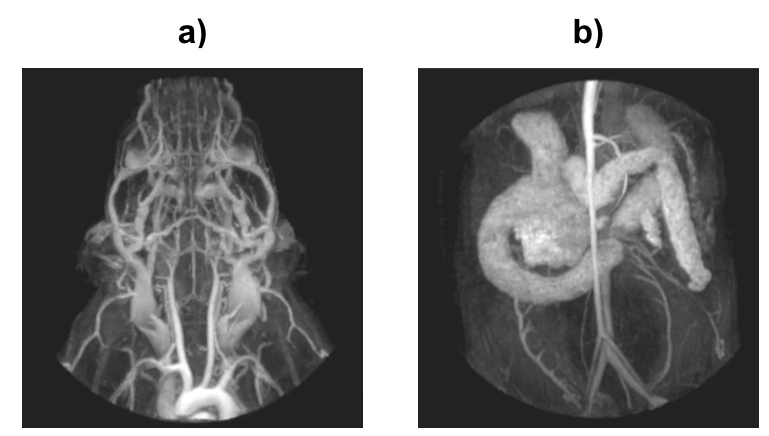
\includegraphics[scale=0.5]{./figure/chap4/UTEUSPIOAnat.png}
\caption[Images anatomiques 3D d'une souris sur différentes zones.]{\label{fig:UTEUSPIOAnat} \textbf{Images anatomiques 3D d'une souris sur différentes zones.} a) Image réalisée en aval de la crosse aortique; b) image réalisée au niveau abdominal.}
\line(1,0){400} \\ 
\end{figure}

La principale limitation de cette méthode d’acquisition est le fait que ce soit une séquence synchronisée sur le rythme cardiaque. La détection des pics ECG ne pose pas dans ce cas de problème car il y a très peu de changement des gradients d’imagerie, par contre, il est nécessaire de stabiliser le rythme cardiaque de l’animal pendant une durée élevée pour obtenir une image de bonne qualité. Cela peut être un problème pour les séquences permettant d’obtenir des images avec une très forte résolution spatiale car celles-ci peuvent durer plus de 35 minutes. Une solution est d’accélérer la séquence pour réduire la probabilité d’avoir des changements de rythme cardiaque importants. Les méthodes d’imagerie parallèle sont difficilement utilisables en pratique préclinique au vue du faible nombre de canaux des antennes, mais il a précédemment été montré que les séquences radiales sont favorables aux algorithmes de reconstruction de type “compressed sensing”. Ceci est une piste à explorer pour réduire les temps d'acquisitions \cite{Nam:2013nx}.
 
 
Cette méthode est \textit{a priori} transposable chez l'homme bien qu'il soit nécessaire de l'adapter à d'autres contraintes. En effet, la séquence est ici seulement synchronisée sur le rythme cardiaque. Hors, chez l’humain, les mouvements respiratoires sont bien plus amples et doivent être corrigés.
Un deuxième point important est que la dose utilisée dans cette étude est supérieure à celle généralement injectée chez l'humain. En l'absence d'informations supplémentaires, il n'est pas possible aujourd'hui d'utiliser de telles concentrations chez le patient. Cependant, des doses entre 50 et 100 $\mu$mol de Fe/kg combinées à la séquence 3D UTE devraient tout de même permettre d'obtenir, particulièrement à des champs $\leq$ à 3T, des images du système vasculaire chez l’humain avec des résolutions temporelles et spatiales supérieures à celles obtenues pour le moment en pratique clinique. Le dernier point problématique à étudier est le temps d’acquisition important de cette séquence supérieur à 30 minutes, qui sera augmenté dans le cas d’une correction de la respiration. Celui-ci pourra être réduit grâce au facteur d’accéleration important pouvant être obtenu en imagerie parallèle. De plus, grâce aux TR particulièrement courts pouvant être utilisés pour cette séquence, il est possible d’associer les projections proches temporellement dans la même image ciné et ainsi accélérer l’acquisition \cite{Trotier2015Time-resolved-T}.
Enfin, il peut être envisager, à la fois en préclinique et en clinique, de développer les techniques d’auto-synchronisation permettant de s’affranchir de l’utilisation de capteurs ECG et de choisir \textit{a posteriori} la résolution temporelle des images. Ces techniques sont tout à fait compatibles avec les méthodes d’encodage radial.

\cleardoublepage
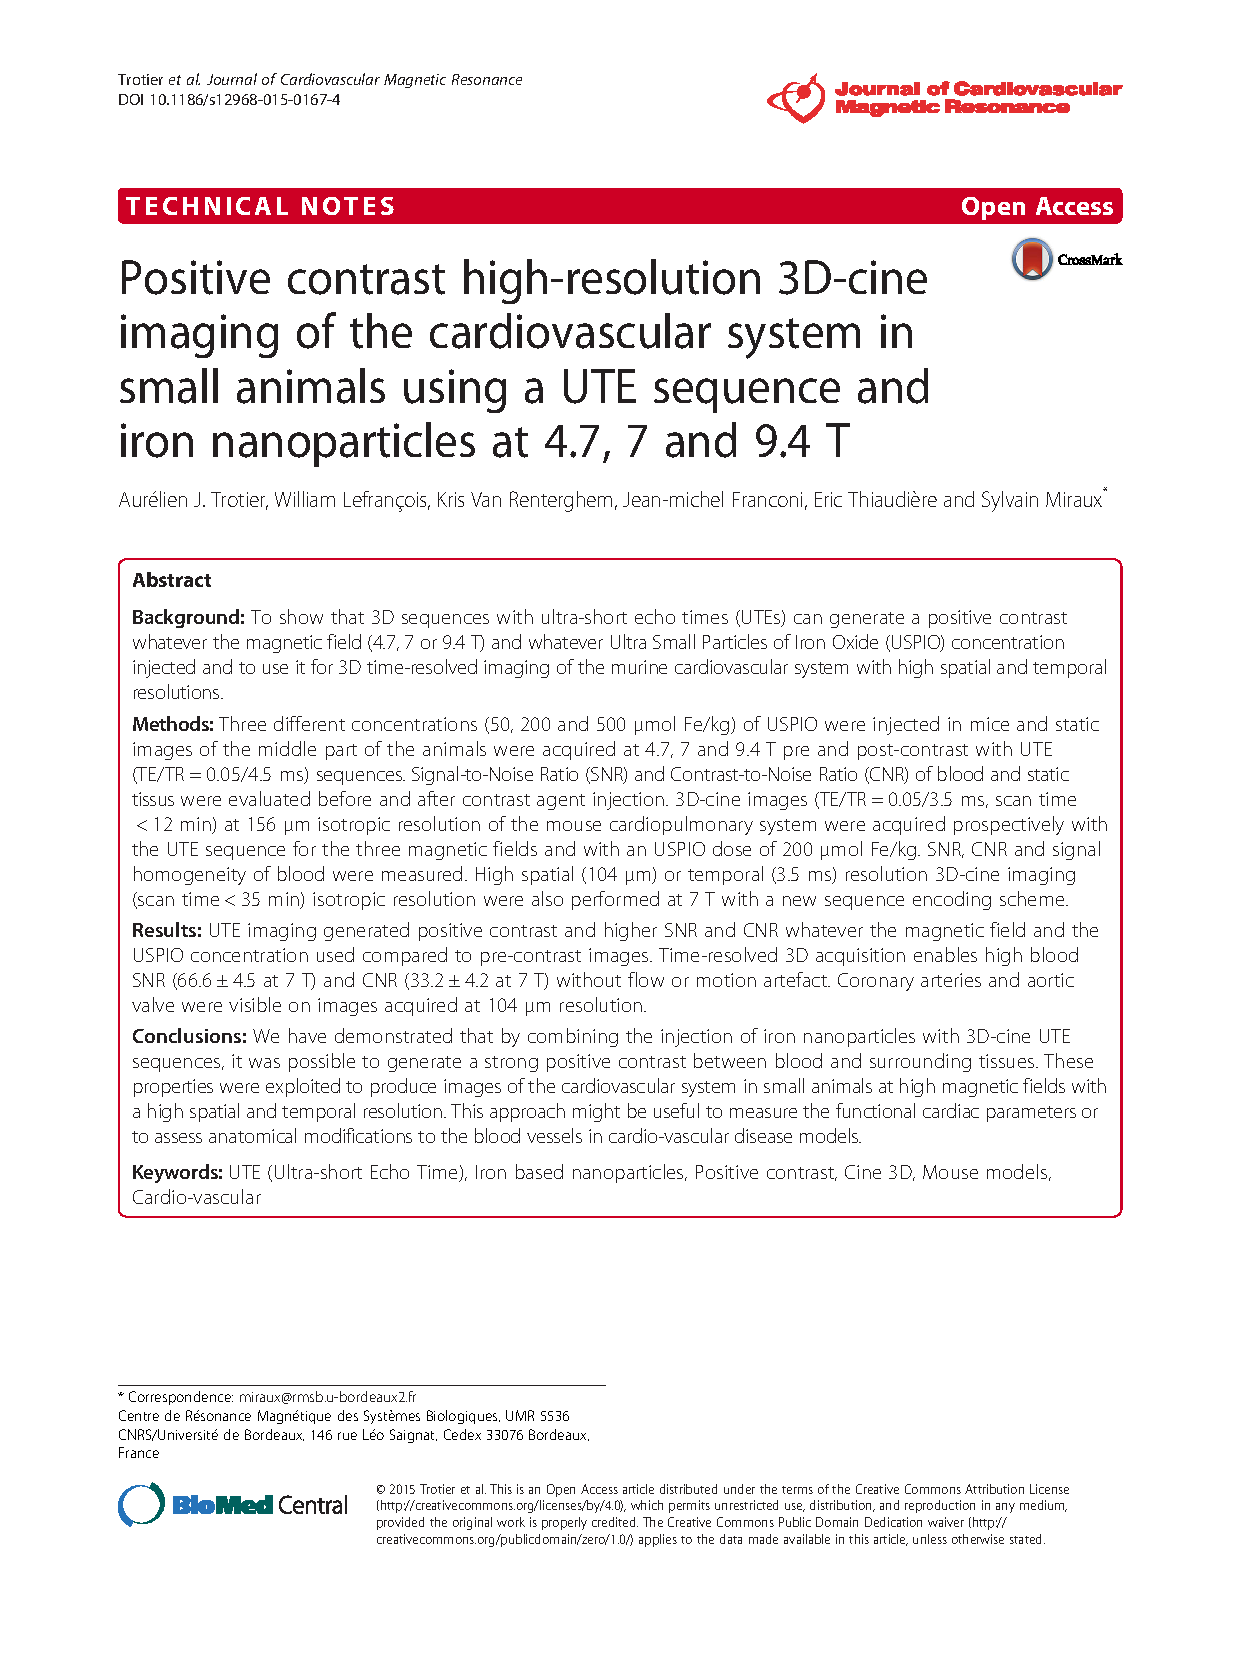
\includepdf[pages=1-10,pagecommand={\thispagestyle{plain}}]{./figure/chap4/Papier2.pdf}







%\chapter{Séquence Stack-Of-Stars UTE auto-synchronisée sur le rythme cardiaque combinée à l'injection de nanoparticules de fer}
\setlength{\footskip}{50pt}
\chaptermark{Angiographie cardiaque autosynchronisée}
\label{Chap5}
\section{Contexte}

L’IRM cardio-vasculaire est devenue la méthode de référence pour l‘évaluation de l’anatomie et de la fonction cardiaque chez la souris. Elle permet de réaliser des images avec de fortes résolutions spatiale et temporelle et d’excellents contrastes endogènes. De plus, grâce à son caractère non-invasif, elle permet de réaliser un suivi longitudinal de modèles de pathologie et ainsi obtenir des informations sur leurs progressions ou l’effet de médicaments.
Néanmoins, malgré les progrès instrumentaux des systèmes IRM préclinique avec l’utilisation de systèmes de gradient très intenses et d’antennes en réseau, il existe encore de nombreuses limitations pour l’imagerie cardio-vasculaire de modèles animaux d’infarctus du myocarde.

Parmi celles-ci, un ECG fortement dégradé par la pathologie du muscle cardiaque et l’utilisation de gradient de champs magnétiques intenses empêchent une synchronisation cardiaque efficace avec l’acquisition RMN. Pour contrer ce problème, la synchronisation ECG peut être remplacées par des méthodes d’imagerie d’auto-synchronisation sur le rythme cardiaque et/ou le mouvement respiratoire \cite{spraggins1990wireless,kim1990extraction}(appelées self-gating ou wireless). Ces méthodes consistes extraire ces informations à partir du signal RMN recueilli pendant l'acquisition.

En effet, en répétant une mesure sans encodage de phase, il a été démontré qu’une variation de signal synchrone avec le mouvement cardiaque peut être extraite des données brutes RMN. L’amplitude du pic de signal RMN (en magnitude ou phase) évolue en fonction du moment dans le cycle cardiaque \cite{Larson2004Self-gated-card,crowe2004automated}. Cette variation du signal est provoqué par le mouvement du myocarde et surtout par le signal du sang intense obtenu grâce à un fort effet temps de vol. Ces méthodes d'auto-synchronisations permettent une reconstruction retrospective des images en fonction du cycle cardiaque et sans artefact de respiration. Elles ont été utilisées à la fois chez le petit animal \cite{hiba2006cardiac,Heijman:2007aa,Hiba:2007aa,Bovens:2011aa} et chez l’homme \cite{Larson:2005aa,crowe2004automated,ingle2015self}, et plus récemment ont bénéficié de la flexibilité offerte par les méthodes d’imagerie radiale associées à un encodage pseudo-aléatoire de l’espace de Fourier \cite{Konstandin:2011fk,kramer2014retrospective,kramer2015self,paul2015high,Motaal:2015aa}. 

Les autres difficultés de l’imagerie des modèles d’infarctus du myocarde sont liés à la physiologie de l’animal comme la fréquence élevée des battements cardiaques ou bien la vitesse du sang importante dans les vaisseaux qui engendrent des artefacts de mouvements et de flux. De plus, la très faible taille des structures à observer requière l’acquisition d’images à haute résolution spatiale. Ainsi, imager le coeur dans son entier (de la base à l’apex), peut requérir un temps d’acquisition élevé peu compatible avec l’observation d’animaux fragiles.

Il a récemment été montré que les méthodes d’acquisition radiale à temps d’écho ultra-court (UTE) permettaient de s’affranchir de nombreux artefacts, en particulier les artefacts de flux et de mouvements, mais aussi les artefacts de susceptibilité souvent importants à hauts champs magnétiques \cite{Hoerr:2013gf,Motaal:2015aa,trotier2015positive}. En 2D, elles sont également compatibles avec les méthodes rétrospectives d’auto-synchronisation sans aucune modification puisque le premier point de chaque projection acquis contient toutes les informations de mouvement \cite{ Hoerr:2013gf}.
Néanmoins, cette technique n’a jamais été utilisé en 3D, pourtant l'acquisition d'images avec des résolutions isotropes devrait permettre d’obtenir des mesures de volumétrie plus précises que l’imagerie 2D multi-coupes \cite{sorensen2005three} et ainsi permettre de mieux décrire les modèles pathologiques.

Ils existent de nombreuses séquences 3D permettant d’encoder le signal du centre de l’espace de Fourier vers l’extérieur et ainsi obtenir des TE courts comme l'empilement d'étoiles UTE (Stack-of-Stars UTE : 3D-SOS UTE) \cite{glover1992projection}, UTE 3D avec un échantillonnage de type oursin (Kooshball) \cite{glover1992boron}, l'empilement de spirales (Stack-Of-Spirals) \cite{irarrazabal1995fast}, 3D projection-tornade (twisted-projection-imaging: TPI) \cite{boada1997fast} et cones 3D \cite{Gurney:2006fk}. A hauts champs magnétiques, il est préférable d’utiliser les séquences dans lesquels le temps de lecture du signal est le plus court possible, c’est a dire, les séquence UTE 3D ou 3D-SOS UTE.

La premiere méthode permet d'effectuer des acquisitions isotropes et d’obtenir des temps d’echo les plus courts puisqu’elle ne nécessite pas l’utilisation d’un gradient de sélection de coupe. En revanche, elle est limitée à l’acquisition de champ de vue sphérique et engendre des temps d’acquisitions longs pour satisfaire au critère de Nyquist.
La seconde méthode est une méthode hybride radiale-cartésienne puisqu’elle utilise un encodage dans le plan 2D radial, une sélection de coupe et un encodage de coupe cartésien dans la 3ème dimension (voir \ref{Chap2}). Cette séquence engendre des temps d’echo plus long que la séquence de type UTE 3D. En revanche, un des avantages de cette méthode est qu’une résolution importante peut être obtenue dans le plan sans augmenter le volume couvert \cite{kadbi20154d}. L’autre avantage, est que la sélection d’une coupe (volume) doit permettre d’obtenir une variation de signal RMN plus importante permettant l’auto-synchronisation.

Dans ce chapitre, nous présenterons une séquence 3D-SOS UTE résolue dans le temps combinant auto-synchronisation et encodage pseudo-aléatoire avec un angle d'or 2D entre les projections du plan. La qualité du signal d’auto-synchronisation est comparée à une séquence UTE 2D classique. Un agent de contraste à base de nanoparticule de fer avec une longue rémanence vasculaire est ensuite utilisé pour générer un contraste positif important entre le sang et le myocarde en 3D. La robustesse du sous-échantillonnage de l’espace de Fourier est également évaluée afin de limiter le temps d’acquisition chez les animaux. Enfin, l’intérêt d'une technique 3D avec une haute résolution spatiale est ensuite montré  par des mesures des paramètres fonctionnelles sur les différentes zones du coeur entre des animaux sains et des animaux avec un infarctus du myocarde.



\section{Séquence Stack-Of-Star UTE auto-synchronisée sur le rythme cardiaque.}

\subsection{Chronogramme de la séquence}

La séquence Stack-Of-Star UTE combine une trajectoire UTE 2D à un encodage 3D cartésien dans la troisième dimension. Cette trajectoire fait apparaitre des artéfacts de type "streaking" du même type que ceux en 2D pour les forts facteurs de sous-échantillonnage comme illustré dans la figure \ref{fig:SoSUTE} mais elle permet de réduire le champ de vue dans la direction de coupe par rapport à la séquence UTE 3D. Cette propriété est nécessaire pour permettre d'obtenir une variation du signal suffisante provoquée par la contraction du coeur. Le deuxième point intéressant de cette trajectoire est son faible temps d'écho (inférieur à 600 $\mu s$) qui permet avec les concentrations de nanoparticules de fer injectées d'obtenir un contraste positif. De plus cela permet aussi d'obtenir des images moins impactée par les artéfacts de déphasage de flux par rapport à une séquence cartésienne \cite{Hoerr:2013gf}.

\begin{figure}[H]
\centering
\line(1,0){400} \\
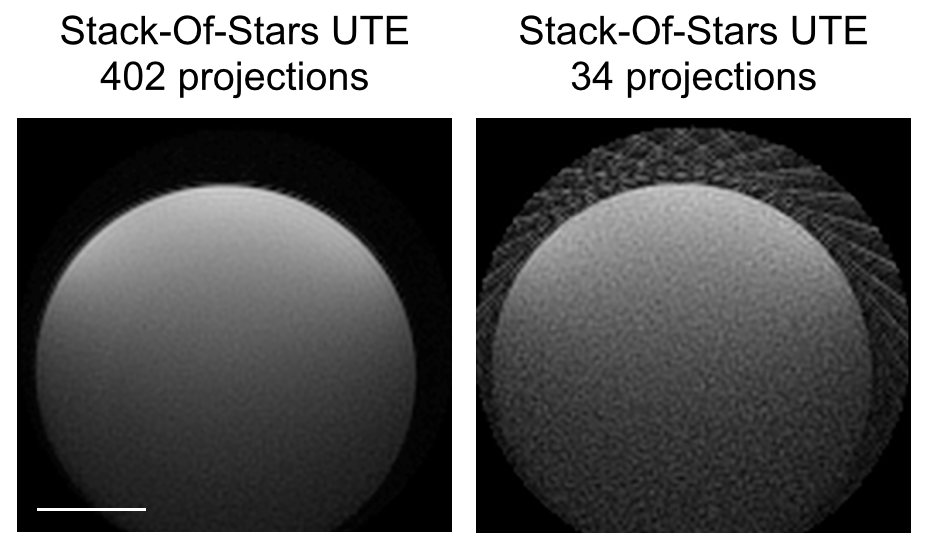
\includegraphics[scale=0.5]{./figure/chap5/Fig1.png}
\caption[Effet du sous-échantillonnage avec une séquence 3D-SOS UTE.]{\label{fig:SoSUTE} \textbf{Effet du sous-échantillonnage avec une séquence 3D-SOS UTE.} Images obtenues sur un fantôme d'eau avec une séquence Stack-Of-Star UTE avec 402 projections à gauche et 34 projections à droite. On observe des artéfacts de "streaking" particulièrement visible en dehors du fantôme. La barre d'échelle mesure 7,5 mm.}
\line(1,0){400} \\ 
\end{figure}

La séquence a été modifiée pour permettre de recueillir un signal d'écho-navigateur et est présentée dans la figure \ref{fig:SeqSoSUTE}. Généralement, les gradients de rephasage de coupe et de codage de phase dans la direction de coupe sont appliqués en même temps. Ici, les deux gradients sont séparés pour permettre de recueillir le signal d'écho-navigateur au centre de l'espace de Fourier entre le gradient de rephasage de coupe et la table d'encodage de coupe. 
Pour minimiser le temps d'écho, la durée des gradients a été optimisé pour obtenir des délais respectivement de 54 $\mu s$ et de 315 $\mu s$.  Le nombre de point à recueillir, indiqué en vert sur la figure \ref{fig:SeqSoSUTE}, peut être modifié pour accumuler le signal. Durant nos expériences celui-ci a été fixé à 3 correspondant à un temps d'acquisition de 30 $\mu s$ (3 x la durée d'acquisition entre deux points).

402 projections ont été recueillies par partition (Stack) dont les trajectoires sont définies selon deux méthodes : i) méthode incrémentale $\Phi = i \times \frac{360\degres}{N_p}$, ii) la méthode d'angle d'or 2D $\Phi = i \times 222.48\degres mod(360\degres)$ où $N_p$ est le nombre de projection par partition selon la direction de coupe. Toutes les projections d'une partition sont recueillies avant le passage vers la partition suivante. 96 partitions ont été recueillies durant nos expériences pour remplir un espace de Fourier cylindrique.

La méthode employée ici étant une stratégie de reconstruction rétrospective, ce schéma d'acquisition est répété un nombre de fois égale au nombre de répétition NR. Lors de cet article les données ont été recueillies avec un nombre ${NR}=10$ puis sous-échantillonnée a posteriori pour évaluer la robustesse de l'acquisition au sous-échantillonnage.

\begin{figure}[H]
\centering
\line(1,0){400} \\
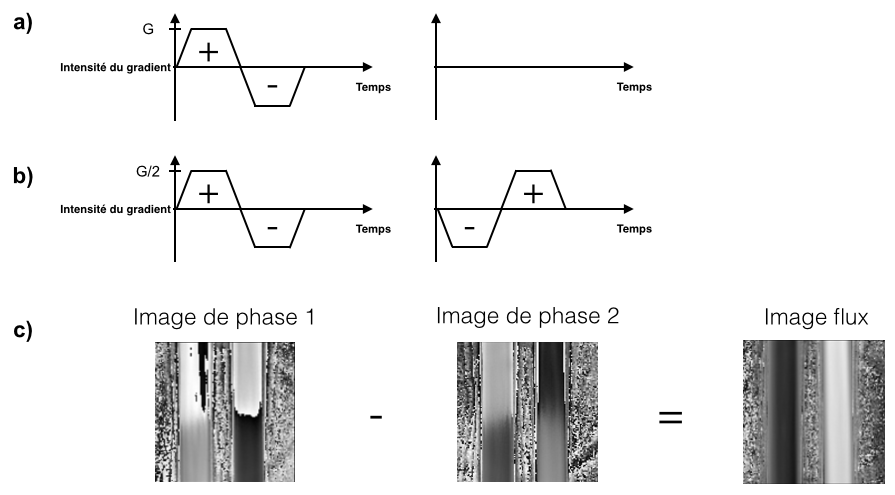
\includegraphics[scale=0.5]{./figure/chap5/Fig2.png}
\caption[Chronogramme de la séquence Stack-Of-Star UTE auto-synchronisée sur le rythme cardiaque.]{\label{fig:SeqSoSUTE}\textbf{Chronogramme de la séquence Stack-Of-Star UTE auto-synchronisée sur le rythme cardiaque.} Le signal d'écho-navigateur (en vert) est recueilli durant le gradient de rephasage de coupe. Le signal utilisé pour la reconstruction est indiqué en rouge est est encodé selon une trajectoire incrémentale ou d'angle d'or 2D.}
\line(1,0){400} \\ 
\end{figure}

\subsection{Traitement du signal d'écho-navigateur.}

Le signal d'écho-navigateur est utilisé pour extraire les mouvements de contraction du coeur a posteriori en utilisant le logiciel MATLAB (MathWorks, Natick, MA).  Les points recueillis sont additionnés de manière complexe pour chaque éléments d'antenne. L'élément permettant d'obtenir la plus grande amplitude de variation de signal est utilisé et son signal convolué avec un filtre gaussien pour limiter les effets du bruit sur la détection des pics (voir figure \ref{fig:Signal}). Le début de chaque cycle cardiaque est déterminé grâce à un algorithme de détection des pics.  L'écart médian entre les pics ainsi que son écart type sont calculés. Les données recueillies entre deux pics qui sont distants de plus 2 fois l'écart type par rapport à la valeur médiane ne sont pas utilisé durant la reconstruction.

Le nombre de volume ciné (NCiné) reconstruit durant le mouvement cardiaque est défini par l'utilisateur. Les données sont regroupées en fonction de leurs positions relatives entre deux pics de l'écho-navigateur dans les espaces de Fourier correspondant au cycle cardiaque permettant ensuite de reconstruire les volumes cinés avec la procédure de reconstruction "gridding" évoqué dans le chapitre \ref{Chap2}.

\begin{figure}[H]
\centering
\line(1,0){400} \\
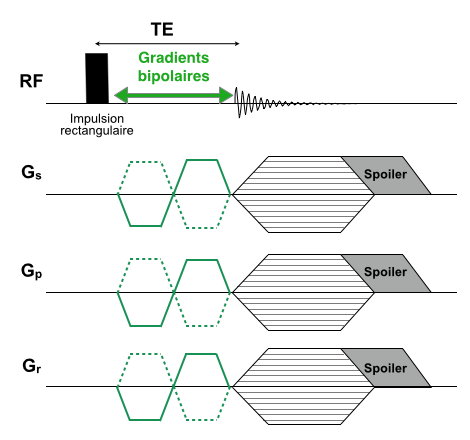
\includegraphics[scale=0.45]{./figure/chap5/Fig3.png}
\caption[Extraction du signal écho navigateur.]{\label{fig:Signal} \textbf{Extraction du signal écho navigateur.} Schéma présentant le signal écho-navigateur cardiaque obtenu durant une acquisition sur une souris avec une séquence \textbf{(a)} UTE 2D sans injection et \textbf{(b)}Stack-Of-Star UTE 3D avant injection et \textbf{(c)} après injection de 200 $\mu mol Fe/kg$. Le signal brut est présenté sur le schéma du haut et après convolution avec un filtre gaussien sur le schéma du bas. Les images axiales du coeur correspondantes sont présentée en bas. La barre d'échelle mesure 5 mm.}
\line(1,0){400} \\ 
\end{figure}

Des exemples de signaux écho-navigateur sont montrés dans la figure \ref{fig:Signal} pour une acquisition 2D et 3D sans injection de produit de contraste et après injection de 200 $\mu mol Fe/kg$. 

Le signal écho navigateur obtenu avec la version 2D de la séquence, sans injection d'agent de contraste, et une épaisseur de coupe de 0,3 mm est montré dans la figure \ref{fig:Signal}.a. Comme décris dans la littérature, le cycle cardiaque et respiratoire peut être extrait des données brutes avec ou sans filtrage et des images peuvent être reconstruite retrospectivement. Quand l'épaisseur de coupe est augmentée pour faire de l'imagerie 3D (figure \ref{fig:Signal}.b), l'amplitude des pics provoquées par le mouvement respiratoire semble comparable à ceux dans imagerie 2D. D'un autre coté, l'amplitude de variation de signal provoquée par le mouvement cardiaque est diminuée et le niveau de bruit est fortement augmenté. Dans certain cas, le signal peut être filtré et permet d'obtenir une visualisation suffisement précise des pics pour permettre d'assigner les projections dans les cycles cardiaques correspondants comme montré sur la figure \ref{fig:Signal}.b. Cependant, dans certaines expériences le niveau de bruit est trop important et empêche une détection précise des pics et donc une reconstruction retrospective. Une fois de plus, le problème majeur avec les acquisitions 3D est l'absence de signal sanguin dans le ventricule droit ($\text{SSB}= 9,57 \pm 2,19$ et $\text{CSB}= -7,82 \pm 2,05$) provoqué par la saturation du signal du sang. De plus, cette absence de contraste empêche d'effectuer des analyses de volumétrie cardiaque.
Après l'injection d'un agent de contraste à base de nanoparticules de fer, le signal sanguin dans les deux ventricules est rehaussé ($\text{SSB}= 42,25 \pm 2,19$ et $\text{CSB}= 17,25 \pm 2,34$) comme montré dans la figure \ref{fig:Signal}.c. La variation d'amplitude provoqué par le mouvement cardiaque est alors augmenté et le bruit est faible par rapport au signal sans agent de contraste. Des images cinés peuvent être reconstruitent après que les projections aient été assignées au cycle cardiaque correspondant, ces images peuvent être utilisées pour effectuer des analyses de la fonction cardiaque. Entre 5 et 10  pourcents du nombre total de projections acquises durant l'expérience sont généralement rejetées à cause d'une trop grande déviation par rapport au rythme médian. Le rythme cardiaque médian mesuré sur les souris saines dans les expériences a été de $412 \pm 32$ et $370 \pm 53$ pour les souris ischémiques.

\section{Répartition des projections incrémentale ou selon l'angle d'or 2D.}

Dans le cas d'une reconstruction rétrospective la méthode de répartition des projections au cours du temps a une influence sur le résultat. Par exemple dans le cas de la suppresion des projections corrompues par la respiration, avec une trajectoire incrémentale une partie de l'espace de Fourier n'est pas rempli car les projections sont adjacentes alors qu'avec une trajectoire aléatoire, ces suppressions de projection sont réparties dans tout l'espace de Fourier et non pas centralisée autour d'une position. 

Pour valider cette affirmation dans le cas d'une séquence cardiaque 3D avec une trajectoire basée sur l'angle d'or 2D, une analyse de la densité de l'espace de Fourier a été effectuée en fonction des méthodes d'encodage (méthode incrémentale versus angle d'or 2D). Deux paramètres ont été étudiés : L'angle moyen et l'écart type entre les projections les plus proches dans chaque partition à l'intérieur des partititions. Cette analyse a été effectuée sur des données acquises \textit{in vivo} sur 4 souris saines pour obtenir 10 images cinés, retrospectivement sous-échantillonnées (de $NR = 10$ à $NR = 1$).

La figure \ref{fig:GoldVSIncNr}.a montre la valeur moyenne de l'angle en fonction du nombre de répétitions. Les deux méthodes permettent d'obtenir des résultats quasi-identiques avec des valeurs inférieurs à 2$\degres$ pour un nombre de répétitions supérieur à 7 puis qui augmentent jusqu'à 9$\degres$ pour une seule répétition. En revanche, en ce qui concerne l'écart-type de la valeur de l'angle, la méthode avec l'angle d'or 2D permet d'obtenir des valeurs toujours plus faibles par rapport à la méthode avec l'angle incrémental. Il est à noté que la dispersion de ces écart-types augmente avec la diminution du nombre de répétition. Cela peut s'expliquer par la différence de rythme cardiaque ainsi que d'efficacité de détection des pics entre les animaux.

\begin{figure}[H]
\centering
\line(1,0){400} \\
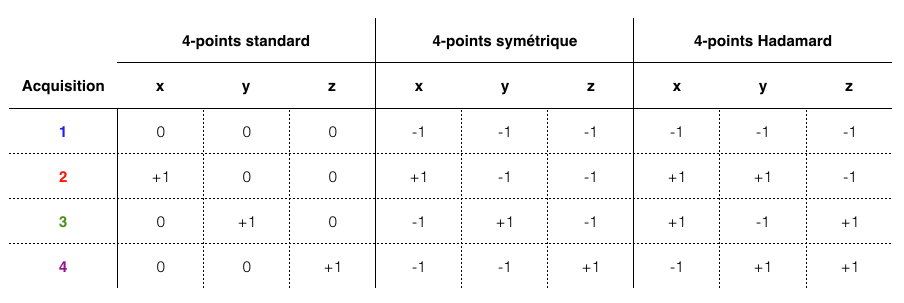
\includegraphics[scale=0.6]{./figure/chap5/Fig4.png}
\caption[Mesure de la densité de répartition des projections.]{\label{fig:GoldVSIncNr} \textbf{Mesure de la densité de répartition des projections.} Graphique représentant \textbf{(a)} la moyenne et \textbf{(b)} l'écart-type des angles entre les projections les plus proches dans une même partition en fonction du nombre de NR utilisé pour la reconstruction. Les paramètres sont affichés pour la répartition incrémentale des projections et selon l'angle d'or 2D.}
\line(1,0){400} \\ 
\end{figure}

Des images réprésentatives reconstruites en vue long et petit axes sont montrées sur la figure \ref{fig:ImGoldVSIncNr} obtenues avec les deux méthodes de répartition des projections sur une souris saines et avec un nombre de répétitions décroissant.

\begin{figure}[H]
\centering
\line(1,0){400} \\
\includegraphics[scale=0.5]{./figure/chap5/Fig5.png}
\caption[Image de l'nfluence de la trajectoire en fonction du sous-échantillonnage]{\label{fig:ImGoldVSIncNr} Images long et petit axes d'un coeur de souris saine reconstruite avec un nombre décroissant de nombre de répétition (NR) avec : \textbf{a)} une répartition incrémentale \textbf{b)} avec l'angle d'or 2D. Une image de différence est aussi présentée sur la dernière ligne. La barre d'échelle mesure 10 mm.}
\line(1,0){400} \\ 
\end{figure}

Avec le nombre maximum de répétitions (NR = 10) , les images obtenues sont de qualités comparables. Le sang à l'intérieur du coeur apparaît avec un signal parfaitement homogène et sans artefact de flux. Le rapport contraste-sur-bruit entre le sang et le myocarde est d'environ 15 avec les deux méthodes (figure \ref{fig:TabGoldVSIncNr}). En diminuant le nombre de répétitions, la qualité des images décroît plus rapidement avec la méthode incrémentale. Ceci est également visible sur les images de différences obtenues par soustraction de l'image avec NR = 10 avec les images obtenues avec des NR plus faibles.
La résolution spatiale des images est dégradée et le contraste sur bruit entre le sang et le myocarde diminue plus fortement sur les images obtenues avec l’angle incrémental (figure \ref{fig:TabGoldVSIncNr}). En diminuant nettement le nombre de répétitions (NR = 2 et 1), la visualisation des ventricules et des parois du myocarde reste possible avec la méthode d'angle d’or 2D mais impossible avec l’autre méthode.

\begin{figure}[H]
\centering
\line(1,0){400} \\
\includegraphics[scale=0.6]{./figure/chap5/Fig6.png}
\caption[Tableau des valeurs de CSB entre les méthodes de répartition d'angle d'or 2D et incrémentale.]{\label{fig:TabGoldVSIncNr} \textbf{Tableau des valeurs de CSB entre les méthodes de répartition d'angle d'or 2D et incrémentale.} Les mesures de CSB ont été effectuées entre le sang et le myocarde pour différentes valeurs de sous-échantillonnage (NR = 10 à 1).}
\line(1,0){400} \\ 
\end{figure}


La flexibilité de cette méthode d'auto-synchronisation permet d'augmenter le nombre d'images cinés reconstruites à partir d'un même jeu de donnée. La figure \ref{fig:GoldVSIncNCine} montre l'écart-type de l'angle en fonction en augmentant le nombre d'images cinés avec 10,9,6 et 4 répétitions pour les deux méthodes de répartition des projections. La méthode d'angle d'or 2D reste plus efficace et l'écart de la valeur reste stable entre les deux méthodes jusqu'à un nombre d'images cinés égal à 20. Après cette valeur, les deux techniques présentent des valeurs qui se rapprochent.

\begin{figure}[H]
\centering
\line(1,0){400} \\
\includegraphics[scale=0.4]{./figure/chap5/Fig7.png}
\caption[Quantification de l'écart-type des angles en fonction de nombre d'images cinés reconstruitent.]{\label{fig:GoldVSIncNCine} \textbf{Quantification de l'écart-type des angles en fonction de nombre d'images cinés reconstruitent.} Graphique représentant  l'écart-type des angles entre les projections les plus proches dans une même partition en fonction du nombre de volumes cinés reconstruits pour la répartition incrémentale et selon l'angle d'or 2D. Les mesures sont représentées en fonction de nombre du nombre de répétition (NR) utilisé pour la reconstruction.}
\line(1,0){400} \\ 
\end{figure}

\section{Imagerie d'un modèle sain de souris versus un modèle d'infarctus du myocarde aiguë versus}

L'imagerie des souris a été effectué à 7 Tesla avec une antenne surfacique à 4 éléments. Les paramètres d'acquisitions sont les suivants :
TR/TE = 4/0.552 ms, type d'excitation radiofréquence/durée/angle d'excitation = hermite/0,3 ms/15$\degres$, champ de vue = 20 x 20 x 15, matrice dans le plan = 128 x 128, nombre de partition = 96, nombre de projection par partition = 402, bande passante de réception = 781 Hz/Pixel, nombre de répétition = 10, temps d'acquisition total : 25 min 43 sec, 3 points recueillis pour l'écho navigateur.

Des souris OF1 saines (n=4) et avec un infarctus du myocarde (n=4) avec un poids compris entre 37 et 40g ont été imagées. Les souris ont été injectées avec un volume de 150 $\mu L$ de Sinerem (Guerbet, Aulnay-sous-bois, France) à une concentration de 200 $\mu mol$ Fe/kg avant le positionnement dans l'imageur.

\newpage
\subsection{Qualité des images}

La figure \ref{fig:ImSaine} montre les 10 images cinés en orientation long et petit axes obtenues chez une souris saine avec un nombre de répétitions égale à 6. La figure \ref{fig:ImInfarct} montre les images obtenues sur une souris avec une ischémie sévère du myocarde. La vue long axe est montrée sur la première ligne (\ref{fig:ImInfarct}.a) et des coupes aux positions b,c et d (indiquées sur la figure \ref{fig:ImInfarct}.a.1) sont montrées sur les autres lignes.

Sur les deux types de souris, le sang apparaît avec un signal intense et homogène sans artefact de flux, quel que soit le moment du cycle cardiaque. Grâce à l'acquisition 3D, l'entièreté de la zone ischémiée peut être délimitée sur les différentes orientations des images (voir flèches sur la figure \ref{fig:ImInfarct}).

\begin{figure}[H]
\centering
\line(1,0){400} \\
\includegraphics[scale=0.5]{./figure/chap5/Fig8.png}
\caption[Images 3D obtenues sur une souris saine avec la séquence 3D-SOS UTE]{\label{fig:ImSaine} \textbf{Images 3D obtenues sur une souris saine avec la séquence 3D-SOS UTE.} Images ciné 3D (orientation long axe et orientation petit axe) obtenues chez une souris saine avec la séquence 3D-SOS UTE auto-synchronisée, la répartition des projections par la méthode de l’angle d’or 2D et un nombre de répétitions NR = 6.}
\line(1,0){400} \\ 
\end{figure}

\begin{figure}[H]
\centering
\line(1,0){400} \\
\includegraphics[scale=0.6]{./figure/chap5/Fig9.png}
\caption[Images 3D obtenues sur une souris avec un infarctus du myocarde avec la séquence 3D-SOS UTE.]{\label{fig:ImInfarct} \textbf{Images 3D obtenues sur une souris avec un infarctus du myocarde avec la séquence 3D-SOS UTE.} Images ciné 3D obtenues chez une souris avec un infarctus du myocarde avec la séquence empilement d’étoiles UTE auto-synchronisée; la répartition des rayons par la méthode de l’angle d’or et un nombre de répétitions NR = 6. Ligne a) orientation long axe. La position des coupes montrées en b) c) et d) apparait sur l’image 1.a). Les flèches indiquent la zone ischémique.}
\line(1,0){400} \\ 
\end{figure}


\subsection{Quantification de la fonction cardiaque.}

Les volumes du ventricule gauche en fin de diastole et de systole ont été mesuré puis la fraction d'éjection calculée à partir des images acquises sur les souris saines et pahtologiques. Les valeurs moyennes de la fraction d'éjection, du volume de fin de diastole et de fin de systole du ventricule gauche apparaissent fortement différentes entre les deux types de souris pour la valeur NR = 10 (voir figure \ref{fig:TabFractionEjection})

\begin{figure}[H]
\centering
\line(1,0){400} \\
\includegraphics[scale=0.5]{./figure/chap5/Fig10.png}
\caption[Tableau des volumes et fractions d'éjection pour les souris saines et pathologiques.]{\label{fig:TabFractionEjection} \textbf{Tableau des volumes et fractions d'éjection pour les souris saines et pathologiques.} Valeurs moyennes de la fraction d’éjection, du volume de fin de diastole et du volume de fin de systole obtenues chez les souris saines et les souris avec un infarctus du myocarde.}
\line(1,0){400} \\ 
\end{figure}

Les mesures ont aussi été réalisées sur les images reconstruites avec NR = 6 et 3. Les données avec NR = 10 ont été prises comme référence. Les données obtenues avec NR : 6 sont extrêmement proches des données obtenues avec NR : 10 pour les deux types de souris. En revanche, avec NR = 3 les données obtenues sur souris saines apparaissent plus dispersées comme le montre le graphie de Bland-Altman sur la figure \ref{fig:BlandAltmanFractionEjection}.

\begin{figure}[H]
\centering
\line(1,0){400} \\
\includegraphics[scale=0.4]{./figure/chap5/Fig11.png}
\caption[Graphique de Bland-Altman de la fraction d’éjection.]{\label{fig:BlandAltmanFractionEjection} \textbf{Graphique de Bland-Altman de la fraction d’éjection.} Graphique de Bland-Altman de la fraction d’éjection pour NR = 6 et NR = 3 en comparaison à NR = 10. Les carrés pleins indiquent les souris saines et les ronds vides les souris avec infarctus du myocarde.}
\line(1,0){400} \\ 
\end{figure}

\subsection{Quantification de la fonction cardiaque en fonction de la zone cardiaque.}

Grâce au caractère 3D des données et aux résolutions isotropes obtenues, les analyses volumiques et de fractions d'éjection peuvent être réalisées coupe à coupe du haut jusqu'au bas du coeur.
Pour la souris saine montrée sur la figure \ref{fig:FractionEjectionCoupe}.a le coeur est ainsi divisé en 40 coupes. La fraction d'éjection apparaît constante tout le long du grand axe et avec des valeurs aux alentours de la fraction d'éjection moyenne. Des profils identiques ont été observés sur les autres souris saines.

Pour la souris avec un infarctus du muocarde montrée sur la figure \ref{fig:FractionEjectionCoupe}.b, le coeur est divisé en 55 coupes. La valeur de fraction d'éjection dans le haut du coeur est comparable à la souris saines environ jusqu'à la coupe 15. Elle dominue ensuite fortement pour être nulle à partir de la coupe 40.

\begin{figure}[H]
\centering
\line(1,0){400} \\
\includegraphics[scale=0.5]{./figure/chap5/Fig12.png}
\caption[Analyse de la fraction d'éjection en fonction de la position dans le coeur.]{\label{fig:FractionEjectionCoupe} \textbf{Analyse de la fraction d'éjection en fonction de la position dans le coeur.} Analyse de la fraction d’éjection en fonction de la position dans le coeur. a) souris saines, b) souris avec un infarctus du myocarde. Le segment sur les images représente l’axe de position des coupes.}
\line(1,0){400} \\ 
\end{figure}

\section{Discussion}


Une méthode d’imagerie 4D pour la mesure de la fonction du ventricule gauche chez la souris a été développée et utilisée pour la caractérisation de souris saines et de souris atteintes d’un infarctus sévère du myocarde.
La méthode se base sur un encodage hybride, radial à temps d’écho ultra-courts dans la dimension du plan et cartésien dans la dimension de coupe. 

L’utilisation de l’encodage cartésien dans la 3ème dimension a plusieurs avantages. Le premier est qu’il permet de réaliser une sélection de coupe relativement fine et ainsi obtenir un signal d’auto-synchronisation cardiaque \cite{crowe2004automated}. En effet, avec une méthode UTE purement radiale (3D-UTE) le signal d’auto-synchronisation cardiaque est noyé dans le signal d’un large volume, même après injection d’USPIO (donnée non montrée) et il n’apparaît pas assez intense pour extraire le rythme cardiaque de l’animal. Avec la séquence proposée, le signal d’écho navigateur est lu pendant le gradient de refocalisation de coupe. Contrairement au séquences UTE 2D classique, le premier point du signal UTE \cite{Hoerr:2013gf,Motaal:2015aa}, échantillonné au centre de l’espace-k ne peut être utilisé comme echo navigateur. Il est en plus nécessaire d’ajouter une table de codage dans la direction de coupe. Le temps d’écho est ainsi rallongée en 3D. Toutefois, en compressant la séquence et en utilisant des gradients de codage intenses, il a été possible de limiter le temps d’écho à environ 0.5 ms. Avec cette méthode, comme déjà proposé avec les séquences 2D, le signal d’écho navigateur est lus à chaque TR contrairement à certaines études chez l’homme \cite{coppo2014free} et le petit animal \cite{kramer2015self} où le signal de l’echo navigateur n’est lu que périodiquement (tout les 4 ou 10 TR). Cela permet, chez la souris où le rythme cardiaque est extrêmement élevée, d’identifier avec précision le signal de synchronisation cardiaque. 

L’autre avantage de cette séquence utilisant un encodage cartésien dans la direction de coupe est la possibilité de limiter le champs de vue dans la 3eme direction et ainsi le temps d’acquisition. Néanmoins, malgré une coupe limitée en épaisseur, le sang dans les cavités cardiaque apparaît saturé. Il n’est pas possible de visualiser le sang dans le ventricules gauches de l’animal contrairement aux acquisitions en 2D qui avec des coupes environ 10 fois plus fines bénéficient d'un effet temps-de-vol. Comme dans plusieurs autres études réalisées en 3D chez le petit animal, il a donc été nécessaire de rehausser le signal du sang avec un agents de contraste \cite{Bucholz:2008uq,Bucholz:2010aa}. Comme déjà montré précédemment, un agent de contraste à base de fer a été utilisé \cite{trotier2015positive}. En effet, ces agents présente l’avantage d’avoir une forte rémanence vasculaire et de générer un contraste positif avec les séquences UTE, même à hauts champs magnétiques \cite{Gharagouzloo2015Quantitative-co}. Du fait de l’autorisation FDA du Ferumoxytol comme supplément en fer pour les patients victimes d’anémies chroniques, ces agents connaissent un regain d’intérêt pour l’angiographie chez l’homme et l’animal \cite{ruangwattanapaisarn2014ferumoxytol}. L’augmentation de temps d’écho (TE = 0.552 ms) d’un facteur 15 environ avec la séquence proposée ici, par rapport aux travaux publiés récemment (TE = 0.031 ms), a peu d’influence sur le signal généré avec les concentrations utilisées dans cet article. Le sang conserve un signal intense tout au long de l’expérience. En effet, grâce à l’encodage SOS-UTE 3D, le temps d’écho de la séquence reste bien en dessous de la millisecondes. De plus, ce type d’encodage rend la séquence peu sensible aux artefacts de mouvements et aux artefacts de flux, même dans sa version 3D. Une synchronisation respiratoire n’a donc pas besoin d’être mise en place. Ainsi, le signal du sang apparait homogène tout au long du cycle cardiaque et chez les deux modèles de souris. Ceci permet de réaliser une segmentation sans ambiguité et obtenir une mesure précise du volume des ventricules. 

Les séquences à TE ultra-court sont également favorables au sous-échantillonnage. Il n’est ainsi pas nécessaire de générer un espace de Fourier complet pour obtenir une image. Ainsi dans le cas d'une reconstruction retrospective, la combinaison de cette encodage permet de générer des images de bonne qualité sans répondre au critères de Nyquist. Cependant, avec une trajectoire classique de type incrémental, la répartition des projections obtenues n’est pas parfaitement homogène, en particulier avec un nombre de répétitions faibles. Cela se traduit par l’apparition d'artefacts typique de l'encodage radial (artefact de « streaking »).
Afin d’améliorer cette situation, une trajectoire pseudo-aléatoire basé sur l’angle d’or (ou golden angle) de chaque disque a été implanté. Comme montrés ici, l’utilisation de celle-ci en combinaison avec la méthode de reconstruction retrospective permet d’obtenir une répartition plus homogène des rayons a l’intérieur d’un empilement. Ainsi, des images 3D fortement sous échantillonnées peuvent être obtenues avec une meilleure résolution spatiale. Ceci peut être utilisé pour limiter le temps d’acquisition des images, pour compenser des données perdues par un mauvais signal de l’écho navigateur ou enfin pour reconstruire un nombre plus important d’images ciné par cycle cardiaque. Ici, seul un encodage aléatoire a été utilisé a l’intérieur de chaque empilement. Du fait du caractère 3D de la séquence, il pourrait être envisagé d’étendre se caractère pseudo-aléatoire entre les différents empilements pour encore plus limiter les artefacts de reconstruction.

En combinant les différents avantages de la séquence développée, nous avons montré qu’il était possible d’obtenir des images 3D ciné sans synchronisation ECG chez la souris saine et la souris avec un infarctus du myocarde sévère. Le signal d’auto-synchronisation, après injection de nanoparticules de fer, s’est montré de qualité suffisante, même chez les souris avec un infarctus. Des résolutions élevées ont été atteintes dans les 3 dimensions de l’espace et permettent ainsi de décrire le modèles pathologiques beaucoup plus finement que ce qui était jusqu’a aujourd’hui décrit dans la littérature. En effet, en imagerie 2D l’épaisseur de coupe est en général limitée à 800 $mu m$ \cite{Bovens:2011aa,Hoerr:2013gf} Le nombre de coupe utilisé sur le coeur entier est au maximum de 10. Ici, 40 pseudo-coupes reconstruites peuvent être utilisées pour déterminer les paramètres fonctionnelles cardiaques chez les souris saines et 55 chez les souris avec un infarctus du myocarde. Grâce à ces données, la pathologie peut être décrites en détail dans les 3 dimensions du coeur. La méthode utilisée permet également de limiter le temps d’acquisition des séquences, paramètres primordiales lors d’études chez des animaux fragiles. Le nombre de répétitions fixé initialement à 10 (temps d’acquisition = 25 min 43 sec) peut ainsi être limité avec très peu de perte en qualité d’image et ainsi obtenir un temps d’acquisition de 15 min 26 sec pour NR = 6. La mesures des paramètres fonctionnelles restent extrêmement robuste. En diminuant ce nombre de répétitions à 3 (temps d’acquisition = 7 min 52 sec) l’erreur devient plus importante mais reste acceptable. 

En résumé, dans ce travail nous présentons une méthode, rehaussée par des nanoparticules de fer, pour l’imagerie ciné 3D du coeur de souris avec une séquence hybride radiale-cartésienne à TE ultra-court. La technique utilise une méthode d’auto-synchronisation couplée à un encodage pseudo-aléatoire des donnés et permet de mesurer les paramètres fonctionnelles cardiaques chez des souris saines et avec un infarctus du myocarde avec des résolution spatiales encore inégalées et un temps d’acquisition de l’ordre de 15 minutes. 


\section{Limitation}

Plusieurs limitations sont à relever pour cette stratégie :
\begin{enumerate}
\item L'espace de Fourier ne peut être rempli de manière identique au cours du temps pour toutes les acquisitions ce qui peut amener à obtenir des images avec une qualité différente selon les phases cardiaques. Cependant dans nos expériences il s'avère que les différences de variation de rythme cardiaque entre les expériences ont un faible impact sur l'écart-type des angles entre les projections et donc sur l'uniformité de répartition des projections dans l'espace de Fourier excepté lorsque qu'un fort facteur de sous-échantillonnage est appliqué.

\item La position du coeur par rapport aux canaux de l'antenne influence le signal écho-navigateur, il est donc nécessaire de sélectionner le canal optimal permettant la visualisation et l'extraction des pics. Cependant il peut arriver que le signal écho-navigateur soit trop faible et nécessite donc une modification de la position de l'animal ou des paramètres d'acquisitions, par exemple une réduction de champ de vue selon la direction de coupe centrée sur le coeur.
\end{enumerate} 

\section{Perspective}
\begin{enumerate}

\item La principale amélioration à apporter à ce travail se situe au niveau du traitement du signal d'écho-navigateur pour permettre une extraction plus robuste et précise du cycle cardiaque. Plusieurs stratégies sont a explorer comme la convolution avec un autre type de filtre ou bien la corrélation croisée entre les différents canaux de l'antenne.

\item L'amélioration du traitement du signal écho-navigateur peut rendre possible l'utilisation d'une séquence 3D UTE auto-synchronisée sur le rythme cardiaque qui permettrait d'atteindre des temps d'écho ultra-court (inférieur à 0,05 ms) et de réduire encore la sensibilité de la séquence aux mouvements et aux artéfacts de flux.

\item Cette méthode est particulièrement adaptée à l'utilisation de stratégie permettant d'améliorer la résolution spatiotemporels comme les filtres temporelles présenté dans le chapitre \ref{Chap3} ou bien avec des méthodes d'accélération de type kt-space puisque l'aspect rétrospectif permet de remplir de manière "aléatoire" les espaces au cours du temps \cite{Motaal:2015aa}.

\item L'ajout de la troisième dimension permet de multiplier les possibilités de quantification. Cependant des outils de traitement et d'analyse de donnée restent à développer pour permettre des études de plus grande cohorte par exemple dans le cas d'étude visant à quantifier la réponse à des traitements pharmacologiques ou à des méthodes de reperfusion du coeur dans le cas d'infarctus ou d'ischémie.
\end{enumerate}




%\chapter{Imagerie de flux 4D du système cardiovasculaire de la souris rehaussée par des nanoparticules de fer avec une séquence UTE.}
\setlength{\footskip}{50pt}
\chaptermark{Imagerie 4D de mesure de flux}
\label{Chap6}
\section{Contexte}

L'accès à des paramètres fonctionnels de manière non invasive est un des enjeux des méthodes d'imagerie moderne. Leur intérêt en terme de diagnotic et de pronostic a déjà été démontré au travers de nombreuses applications dans le domaine cardiovasculaire chez l'homme. Dans cette thèse, l'intérêt d'une méthode de mesure de flux pour la caractérisation qualitative d'un modèle préclinique de pathologie vasculaire a également été montré.

Parmi les méthodes quantitatives de mesure de flux, l'imagerie de phase 4D (3D + t), "4D Flow MRI" est la plus prometteuse et est actuellement la plus répandue en clinique. Son champ d'applications s'élargit d'année en année avec l'étude de pathologies cérébrales \cite{meckel2008vivo,hope2010evaluation}, rénales \cite{franccois2011renal}, hépatiques \cite{stankovic2010mr}, cardiaques \cite{geiger20114d,markl2011time} ...

Cette méthode est particulièrement intéressante car elle permet à partir d'une même acquisition d'obtenir tout au long du cycle cardiaque : des images en magnitude pour visualiser des modifications anatomiques  \cite{Eriksson:2013aa}, des images de contraste de phase pour visualiser les flux anormaux \cite{Velikina:2010hc}, des cartes de vitesse des flux \cite{Garcia:2014aa} qui peuvent ensuite être utilisées pour calculer d'autres paramètres hémodynamiques comme la différence de pression \cite{Tyszka:2000aa,bock2011vivo} ou les contraintes de cisaillement sur les parois des vaisseaux (Wall Shear Stress : WSS)\cite{Zhao:2009ng}. Cette méthode apparaît donc comme un important outil diagnostique en médecine mais son utilisation en routine clinique reste encore aujourd'hui fortement limitée en particulier à cause des temps d'acquisitions requis importants (10 à 20 minutes sur un coeur entier \cite{Markl:2012pi}).

Les problématiques liées à l'utilisation de cette méthode sont exacerbées dans le cas de l'imagerie préclinique et en particulier chez la souris. En effet, le faible rapport signal-sur-bruit ainsi que le nombre réduit de canaux des antennes à disposition sur les systèmes d'imagerie précliniques limitent l'utilisation de méthodes d'accélération parallèle. Le temps d'acquisition d'une image de flux 4D devient ainsi prohibitif. De plus, la présence de flux importants (supérieurs à 1 $m.s^{-1}$) dans des vaisseaux de petites tailles et avec une anatomie complexe a pour effet de favoriser le déphasage intravoxel des spins et donc l'apparition d'artefacts de perte de signal sur les images. Pour réduire ces artefacts, la méthode la plus simple est de réduire le temps d'écho \cite{staahlberg1994pulse,OBrien:2008aa}. L'amélioration des systèmes de gradients que ce soit en terme d'intensité ou de temps de montée, a permis d'atteindre des valeurs de temps d'écho inférieures à 2 ms en imagerie cartésienne conventionnelle. Néanmoins, ces séquences restent inférieures en terme de qualité d'images (artefacts de mouvement et de flux) par rapport aux séquences d'imagerie radiale.

Nous avons montré dans les chapitres précédents qu’en combinant des séquences à temps d’écho ultracourt (UTE) à une injection d’agent de contraste de type USPIO, il est possible de générer des images avec un très fort rapport signal-sur-bruit pour le sang et un très bon contraste-sur-bruit entre le sang et le myocarde, tout ceci sans artefact de flux ni de mouvement. De plus, ces nanoparticules possèdent une forte rémanence vasculaire, ce qui permet de conserver de forts SSB et CSB pendant au moins 1 heure.

C’est donc logiquement, que la séquence à TE ultracourt a été adaptée pour la mesure de flux par imagerie de phase 4D chez la souris. Pour cela, des gradients bipolaires ont été insérés entre l’impulsion radiofréquence non selective et la lecture du signal. Un schéma d’encodage original a été proposé afin de permettre un meilleur moyennage des vitesses en fonction de l’instant du cycle cardiaque. 
Cette séquence a évidemment été couplée a l’injection de nanoparticules de fer afin de rehausser le rapport signal-sur-bruit du sang. En effet, le bruit sur les cartes de vitesses des flux est inversement proportionnel au signal sur les images en magnitude.

La méthode développée a d’abord été validée sur fantôme. Les mesures de vitesses effectuées ont été comparées à celles mesurées avec une séquence cartésienne sur un fantôme de flux. L’impact de la réduction des valeurs de $T_2^*$ dans le cas de l’utilisation de nanoparticules de fer sur la mesure des vitesses sera évalué. Cette méthode a ensuite été utilisée sur un modèle de souris afin d’évaluer les vitesses de flux à chaque instant du cycle cardiaque sur l’entièreté du système cardio-pulmonaire de l’animal. Des résultats préliminaires ont été obtenus en comparant deux populations de souris, la première exposée à des conditions hypoxiques pendant 3 semaines et l’autre en conditions normales.

%L'utilisation de trajectoires non-cartésiennes permet d'atteindre des temps d'écho encore plus réduits ainsi que de limiter la sensibilité aux artefacts de flux. O'Brien et al  \cite{OBrien:2009ul} ont montré que l'utilisation d'une séquence 2D de mesure de flux basée sur une trajectoire radiale UTE permettait en réduisant le TE à 0.6 ms, d'obtenir des mesures plus précises grâce à la réduction des artefacts de déphasage des spins dans le cas des flux ayant une vitesse rapide.  Janiczek et al \cite{Janiczek:2011qm} ont développé et appliqué une séquence 3D de mesure de flux de type empilement de spiral sur la crosse aortique d'une souris et qui, grâce à l'effet temps-de-vol, permet d'obtenir un rapport signal-sur-bruit suffisant pour dériver le WSS. Ils ont montrés dans cette étude que cette trajectoire permet d'obtenir un meilleur signal-sur-bruit que la séquence cartésienne et est moins sensible aux artefacts de flux dans les régions présentant des vitesses rapides et incurvées. Récemment Kadbi et al \cite{Kadbi:2014uq} ont étudié l'utilisation d'une séquence 3D Stack-Of-Star UTE pour la quantification des flux sténotiques et ont montré que cette stratégie permet d'obtenir des résultats en accord avec les mesures cartésiennes pour les flux lents mais surtout de meilleurs résultats dans les cas des flux rapides.

\section{Stratégie de mesure de flux 4D}

\subsection{Introduction à la mesure de flux par imagerie de phase}

\subsubsection{Encodage de vitesses}

La quantification des flux grâce à la phase en IRM utilise l'ajout d'un gradient bipolaire entre l'excitation radiofréquence et la lecture du signal. La figure \ref{fig:PhaseSpins} montre l'effet du gradient bipolaire d'encodage de vitesses sur des spins fixes et mobiles et en particulier l'accumulation de la phase. On observe qu'à la fin du gradient bipolaire la phase des spins fixes retourne à sa position initiale alors que celles des spins mobiles accumule une différence par rapport à l'état initial qui est directement proportionnelle à leur vitesse.

\begin{figure}[H]
\centering
\line(1,0){400} \\
\includegraphics[scale=0.5]{./figure/chap6/Fig1.png}
\caption[Effet du gradient bipolaire sur des spins fixes et mobiles.]{\label{fig:PhaseSpins} \textbf{Effet du gradient bipolaire sur des spins fixes et mobiles.} Représentation schématique de l'évolution de la phase au cours du temps dans le cas de spins fixes et de spins mobiles sous l'influence d'un gradient bipolaire. L'accumulation de phase des spins mobiles est proportionnelle à leurs vitesses. $T_l$ représente la durée d'un lobe et T l'intervalle de temps entre le départ des deux lobes. }
\line(1,0){400} \\ 
\end{figure}
Si l'on définit la position des spins en fonction du temps de la manière suivante :
\begin{align}
x(t)=x_0 + v_0 t +a_0 t^2 + ... + \frac{1}{n!} \left(\frac{d^n x}{dt^n}\right)_{t=0} t^n
\end{align}
%x(t)=x(0) + x_1 t +\frac{1}{2!} x_2 t^2 + ... + \frac{1}{n!} x_n t^n
où $x_0$, $v_0$ et $a_0$ représente respectivement la position, la vitesse et l'accélération initiale au temps $t=0$ selon la direction du gradient bipolaire. Alors l'accumulation de phase après l'application du gradient bipolaire peut se calculer grâce à l'équation suivante :

\begin{align}
\phi (T) &= \gamma \int_0^T G(t) x(t) dt \\
			 &= \gamma (m_0(T) x_0 + m_1(T) v_0 + \frac{1}{2} m_2(T) a_0 ...)
\end{align}
où m représente le moment du gradient. Le $n^{\text{ième}}$ moment de gradient m est défini par :
\begin{align}
m_n (T) &= \int_0^T G(t) t^n dt			
\end{align}
Le moment du gradient $m_0$ donne des informations sur la position des spins, $m_1$ sur la vitesse, $m_2$ sur l'accélération, etc.
Dans notre cas, on désire mesurer la vitesse des flux, il est donc nécessaire que le moment de gradient $m_0$ soit nul. C'est-à-dire que l'aire globale du gradient bipolaire soit égale à 0 (ce qui est le cas dans la figure \ref{fig:PhaseSpins}). Le moment $m_1$ représenté dans cette figure peut être calculé directement :
	
	\begin{equation}
	\begin{split}
	m_1 &= \int_{t=0}^{T_L} -G \ t \ dt  + \int_{t=T}^{T+T_L} -G \ t \ dt  \\
			&= \frac{G}{2}\left(-T_L^2+(T+T_L)^2-T^2\right) \\
			&=G \ T_L \ T \\
			& = A \ T
	\end{split} 
	\end{equation}	
où $T_L$ correspond à la durée d'un lobe, T à l'intervalle de temps entre le départ des deux lobes et A à l'aire d'un lobe (grisé sur la figure \ref{fig:PhaseSpins}). Ce résultat est ici démontré à partir d'un gradient rectangulaire, mais il est généralisable à n'importe quelle forme de gradient bipolaire en les décomposant en une infinité de rectangle de largeur infinitésimale. Ce résultat s'applique donc aussi aux gradients avec une forme trapézoïdale qui est la forme de gradient la plus couramment utilisée dans les séquences.

L'accumulation de phase $\Phi$ pour un groupe de spins ayant une vitesse constante $v$ est donc égale à :
\begin{equation}
\label{eq:VitessePhase}
\Phi = \gamma A \ T \ v
\end{equation}
Ainsi, en modifiant la valeur de l'intensité du gradient bipolaire ou sa durée d'application, il est donc possible de modifier l'écart de phase résultant des spins mobiles en fonction de leurs vitesses.

\subsubsection{Quantification de la vitesse par imagerie de phase}

Pour mesurer la vitesse des spins, il est nécessaire de supprimer la phase statique des tissus produite par les hétérogénéités du champ magnétique $B_0$. La méthode généralement employée consiste à acquérir deux images de phase avec des intensités de gradient bipolaire différentes et ensuite de les soustraire.

Les deux méthodes les plus employées sont représentées dans la figure \ref{fig:MethodeGradientBip}.a et b. 
La méthode (a) est la méthode initialement proposée. Elle consiste à réaliser une image de phase avec un gradient bipolaire et à soustraire cette image à une autre image obtenue sans gradient bipolaire. Elle est encore souvent utilisée car l’image sans gradient bipolaire est moins sensible aux artefacts de déphasage dus au flux et peut être employée comme image de référence en magnitude.
La méthode (b) consiste à utiliser des gradients d’intensités opposées pour l’acquisition de chacune des images. Elle permet de diviser d’un facteur 2 l’intensité maximum des gradients d’encodage des vitesses par rapport à la méthode (a).
C'est cette méthode (b) décrite dans la figure \ref{fig:MethodeGradientBip}.b qui a été employée pour générer les images montrées dans la figure \ref{fig:MethodeGradientBip}.c. De l’eau circule dans un fantôme de flux (de bas en haut pour le tube de gauche et de haut en bas pour le tube de droite). Après soustraction des deux images acquises, la valeur de la phase apparaît homogène dans les deux tubes et avec une valeur opposée. A partir de cette image, la vitesse du flux peut être précisément mesurée à l'aide de l'équation \ref{eq:VitessePhase}. On trouve pour le tube de gauche une vitesse de : $v=0,2679 \pm 0,0063$ $m.s^{-1}$ et pour le tube de droite : $v=0,2478 \pm 0,0104$ $m.s^{-1}$.

\begin{figure}[h]
\centering
\line(1,0){400} \\
\includegraphics[scale=0.5]{./figure/chap6/Fig2.png}
\caption[Représentation de deux méthodes d'encodage de vitesses.]{\label{fig:MethodeGradientBip} \textbf{Représentation de deux méthodes d'encodage des vitesses.} La méthode \textbf{(a)} consiste à recueillir une première image avec une intensité G et l'autre avec une intensité des gradients nulle. La méthode\textbf{(b)} consiste à inverser la polarisation des gradients bipolaires entre les deux images dont l'intensité utilisée est deux fois moindre que pour la méthode (a). Les deux méthodes permettent d'obtenir la même amplitude de codage des vitesses définies par $\Delta m_1 = m_1(image1) - m_1(image2)$. \textbf{(c)} La soustraction des deux images de phase permet d'obtenir une image de mesure de flux. }
\line(1,0){400} \\ 
\end{figure}

\subsubsection{Vitesse d'encodage}

Lorsque la vitesse des spins est trop importante, il est possible que leurs phases $| \Phi | > \pi$, on observe alors un repliement de la phase qui est problématique pour déterminer la vitesse des spins. Le paramètre de vitesse d'encodage des spins souvent noté VENC pour "Velocity ENCoding" a donc été inventé et est généralement exprimé en c$m.s^{-1}$. Celui-ci est fixé par l'utilisateur et correspond à la vitesse maximum qui peut être encodée sans observer de repliement de la phase. Il est donc défini à partir du moment $\Delta m_1=m_1(image_1)-m_1(image_2)$ :
\begin{align}
\text{VENC} = \frac{\pi}{\gamma | \Delta m_1 |}
\end{align} 

En réalité, l'utilisateur va définir le paramètre VENC qui permettra alors de calculer l'intensité/durée des gradients bipolaires permettant d'obtenir un encodage des vitesses correspondant à cette valeur. Dans le cas des gradients trapézoïdaux présentés dans la figure \ref{fig:MethodeGradientBip} qui sont ceux implémentés dans cette séquence, l'intensité des gradients d'encodage G est définie par :

\begin{align}
G = \frac{\pi}{2 \gamma \ T_L \ T \ \text{VENC}}
\end{align}
En posant r le temps de montée et de descente des gradients et d la durée du plateau des gradients trapezoïdaux, on obtient alors $T_L = d+r$ et $T = d+2r$.

La valeur de VENC choisie par l'utilisateur doit être supérieure à la vitesse maximum supposée pour éviter tout repliement. Mais elle doit aussi être relativement proche des vitesses à observer car le paramètre de vitesse-sur-bruit (VSB) dans les cartes de vitesses (l'équivalent du signal-sur-bruit (SSB)) suit la loi suivante :
\begin{align}
\text{VSB} \propto \frac{V}{\text{VENC}}\text{SSB}
\end{align}
 Généralement le paramètre VENC est choisi de manière à être 30$\%$ supérieur à la vitesse maximum qui peut être observer \textit{in vivo}. 

\subsubsection{Antennes multicanaux et reconstruction des images de mesure des flux}

Pour reconstruire une image réalisée avec une antenne multicanaux, la méthode couramment utilisée consiste à combiner les images en magnitude obtenues avec chacun des canaux par la méthode de racine carrée de somme des carrées. Néanmoins, avec cette stratégie l’information de phase dans l’image finale est perdue.
Deux méthodes peuvent être utilisées pour obtenir des images de phase à partir de l’antenne à 4 canaux que nous avons utilisée.

Soit $I_1$ et $I_2$, des images complexes qui sont acquises avec l'une des stratégies de contraste de phase définies dans la partie précédente. Ces images peuvent être représentées en utilisant leur magnitude (A) et phase ($\Phi$) respectives :
\begin{equation}
\begin{split}
I_1= A_1 . e^{i \Phi_1} \\
I_2= A_2 . e^{i \Phi_2}
\end{split}
\end{equation}
La carte de contraste de phase $\Delta \Phi$ pour une antenne à un élément peut alors se calculer de la manière suivante :
\begin{equation}
\begin{split}
\Delta \Phi &= arg(I_1) - arg(I_2) \\
				  &= arg(A_1e^{i(\Phi_1)}) - arg(A_2e^{i(\Phi_2)}) \\
				  &= \Phi_1-\Phi_2
\end{split}
\end{equation}

Cette équation peut être étendue à des données recueillies avec une antenne multicanaux où l'opération de différence de phase est effectuée après la combinaison de tous les canaux individuellement.

\begin{equation}
\begin{split}
\Phi_1 &= arg( \sum_1^n  A_{1,n} \cdot e^{i \Phi_{1,n}}) \\
\Phi_2 &= arg( \sum_1^n  A_{2,n} \cdot e^{i \Phi_{2,n}}) \\
\Delta \Phi &= \Phi_1 - \Phi_2
\end{split}
\end{equation}

Une autre méthode disponible décrite par Bernstein et al \cite{bernstein1994reconstructions} consiste à effectuer l'opération de différence de phase individuellement pour chaque canal puis d'additionner les données avant de générer la carte de phase :

\begin{align}
\Delta \Phi = arg(\sum_1^n A_{1,n} \cdot A_{2,n} \cdot e^{i(\Phi_{1,n} - \Phi_{2,n})})
\end{align}

Dans ce chapitre, la méthode employée est la méthode de Bernstein qui s'avère donner de meilleurs résultats.

\subsection{Chronogramme de la séquence 4D UTE de contraste de phase}

\begin{figure}[H]
\centering
\line(1,0){400} \\
\includegraphics[scale=0.5]{./figure/chap6/Fig3.png}
\caption[Chronogramme de la séquence 4D UTE de contraste de phase.]{\label{fig:Chrono4DFlux}\textbf{ Chronogramme de la séquence 4D UTE de contraste de phase.} Des gradients bipolaires (en vert) sont présents entre l'excitation radiofréquence non-sélective et la lecture du signal. La polarité et l'intensité des gradients bipolaires sont définies en fonction de la méthode d'encodage des vitesses employée.}
\line(1,0){400} \\ 
\end{figure}

Afin d’encoder les vitesses dans les 3 directions de l’espace et en fonction du rythme cardiaque, une nouvelle séquence d’imagerie de flux a été développée.

Cette séquence décrite dans la figure (\ref{fig:Chrono4DFlux}) est basée sur la séquence 3D UTE présentée dans le chapitre \ref{Chap4}.  Des gradients bipolaires de codage de vitesses (en vert) ont été introduits entre l’impulsion radiofréquence et la lecture du signal. La lecture du signal se fait de manière radiale en partant du centre de l’espace de Fourier. La trajectoire des projections (qui sont des rayons dans le cas des séquences UTE)  est la même que celle décrite dans le chapitre \ref{Chap4}, elle permet de positionner les derniers points de chaque projection en suivant une trajectoire spiralée sur la surface d'une sphère.

En utilisant des intensités de gradients élevées, il est possible de limiter le temps d’applications des gradients bipolaires. Dans notre cas, des valeurs de VENC de 0.6 $m.s^{-1}$ peuvent être atteintes pour une durée de gradient de 0,421 ms correspondant à des intensités de gradients de 52 $\%$ par rapport à l'intensité maximum des gradients de 660 $mT.m^{-1}$. Associé à la durée réduite de l'impulsion de radiofréquence, les valeurs de TE obtenues restent faibles entre 0.450 et 0.550 ms. Les avantages liés au temps d'écho ultracourt restent ainsi vrais pour cette séquence.

\subsubsection{Gradients de codage de vitesses}

Les gradients bipolaires utilisés dans ce travail sont des gradients trapézoïdaux définis par leurs temps de montée \textbf{\textit{r}}, la durée du plateau \textbf{\textit{d}} et l’intensité maximum \textbf{\textit{G}}. La polarité du premier lobe peut être positive ou négative correspondant respectivement aux traits pointillés et pleins sur la figure \ref{fig:Chrono4DFlux}.

Pour mesurer la vitesse selon les 3 directions de l'espace, il est nécessaire d'encoder les vitesses selon les 3 axes. Ceci requiert au minimum 4 acquisitions avec des combinaisons de gradients bipolaires différentes. Plusieurs combinaisons de gradients bipolaires peuvent être utilisées \ref{fig:EncFlux} : 4-points standard, 4-points symétrique, 4-points Hadamard. 

\begin{figure}[H]
\centering
\line(1,0){400} \\
\includegraphics[scale=0.45]{./figure/chap6/Fig4.png}
\caption[Présentation de 3 méthode d'encodage de flux.]{\label{fig:EncFlux} \textbf{Tableau représentant la polarité des gradients bipolaires pour 3 méthodes} : 4-points standard, 4-points symétrique et 4-points Hadamard. Pour obtenir le même encodage des vitesses pour la méthode standard, l'intensité des gradients bipolaires est 2 fois plus importante que pour les deux autres méthodes.}
\line(1,0){400} \\ 
\end{figure}

\subsubsection{Reconstruction des cartes de vitesses}

Pour obtenir les cartes de vitesses à partir des reconstructions de chaque acquisition, la combinaison des données est différente en fonction de la méthode de codage employée. Pour les méthodes standard et symétrique, les cartes de vitesses ($V_x,V_y,V_z$) sont obtenues en combinant les cartes de phase des acquisitions, notées $Acq_i$ (i=1, 2, 3 ou 4) selon la méthode suivante :

\begin{equation}
\begin{split}
V_x = (Acq_2-Acq_1) \frac{\text{VENC}}{\pi} \\
V_y = (Acq_3-Acq_1 ) \frac{\text{VENC}}{\pi}\\
V_z = (Acq_4-Acq_1 ) \frac{\text{VENC}}{\pi}
\end{split}
\end{equation}

Pour la méthode d’encodage Hadamard, chaque carte de vitesses ($V_x$, $V_y$, $V_z$) combine toutes les données acquises selon la méthode suivante : 

\begin{equation}
\begin{split}
V_x = (-Acq_1+Acq_2+Acq_3-Acq_4) \frac{\text{VENC}}{\pi} \\
V_y = (-Acq_1+Acq_2-Acq_3+Acq_4 ) \frac{\text{VENC}}{\pi}\\
V_z = (-Acq_1-Acq_2+Acq_3+Acq_4 ) \frac{\text{VENC}}{\pi}
\end{split}
\end{equation}

Les méthodes 4-points symétrique et Hadamard ont été testées. En effet, elles permettent de réduire l’intensité maximale des gradients d’un facteur 2 par rapport à la méthode standard pour la même valeur de VENC. Il est donc possible en utilisant 100 pourcents de l'intensité des gradients de réduire la durée des gradients de codage de vitesses et par conséquent le temps d’écho de la séquence.

Finalement, le choix définitif s'est porté sur la méthode symétrique. En effet, la plage dynamique des vitesses qui peuvent être mesurées avec la méthode Hadamard sans obtenir de repliement est dépendante de la direction de la vitesse des flux. Il est ainsi possible d'obtenir un repliement de la phase si la vitesse est supérieur à $v=\text{VENC}/\sqrt{2} $ selon 2 directions d'encodage des vitesses \cite{Pelc:1991aa} contrairement à la méthode d'encodage symétrique.

\subsection{Stratégie d'encodage 4D de vitesses des flux}

Pour mesurer les vitesses de flux en fonction du cycle cardiaque, la séquence est synchronisée prospectivement sur l’onde R de l'ECG. Au cours d'un cycle cardiaque, NCine phases sont reconstruites (Ciné 1, Ciné 2, ..., Ciné N). Chaque phase est reconstruite à partir de 4 signaux IRM permettant d'encoder la vitesse selon les 3 dimensions avec la méthode 4-points symétrique. Tous les signaux recueillis au cours du même battement de coeur ont la même trajectoire, celle-ci est définie selon la méthode présentée dans le chapitre \ref{Chap4}. Les couleurs des signaux IRM qui sont représentées sur la figure \ref{fig:SchemaAcqFlux} permettent de définir la polarité des gradients bipolaires qui sont utilisés en accord avec les couleurs des acquisitions représentées dans la figure \ref{fig:EncFlux}. 

L'ordre d'encodage des signaux IRM dans chaque phase cardiaque est déplacé d'une étape à chaque battement de coeur, puis réinitialisé après le 4$^\text{ème}$ battement. Cette stratégie permet de recueillir à chaque battement de coeur les projections permettant d'encoder les trois directions avec une même trajectoire. Le changement d'ordre d'encodage d'un battement cardiaque à l'autre permet quant à lui de moyenner le mouvement et les modifications de vitesses sur les phases cardiaques qui seront reconstruites.

\begin{figure}[H]
\centering
\line(1,0){400} \\
\includegraphics[scale=0.5]{./figure/chap6/Fig5.png}
\caption[Schéma acquisition des données de flux 4D.]{\label{fig:SchemaAcqFlux} \textbf{Schéma d'acquisition des données de flux 4D.} Les acquisitions sont synchronisées prospectivement sur le rythme cardiaque. Chaque couleur de FID correspondant à l'utilisation de gradient bipolaire en accord avec la figure \ref{fig:EncFlux}.}
\line(1,0){400} \\ 
\end{figure}

\subsection{Correction des erreurs de phase/vitesse}

Lors de l'acquisition des images de flux, des erreurs de phase sont souvent observées et engendrent des erreurs sur les mesures de flux. Ces erreurs proviennent principalement de 3 sources : les courants de Foucault \cite{Walker:1993aa}, les gradients concomittants \cite{Bernstein:1998aa} et les distorsions du champ de gradient provenant de la géométrie des bobines de gradients. \cite{Markl:2003aa}. 

Diverses méthodes existent pour corriger ces erreurs. Dans ce chapitre la méthode décrite par Chernobelsky et al \cite{Chernobelsky:2007aa} a été implémentée car elle permet de corriger les erreurs provoquées par les courants de Foucault et les gradients concomittants. Cette méthode consiste à appliquer la même séquence d'imagerie de flux (avec les mêmes paramètres) sur un fantôme homogène statique, puis de soustraire les cartes de vitesses obtenues avec ces données aux cartes de vitesses obtenues \textit{in vivo}. 

Un exemple d'application de cette stratégie de correction est présenté dans la figure \ref{fig:CorrectionPhase}. Sur l'image acquise non corrigée, la présence d'une erreur linéaire sur la carte de vitesses est observée (ligne pointillée). Après soustraction des images \textit{in vivo} avec l'image acquise sur le fantôme statique, l'erreur linéaire est corrigée et la vitesse apparaît uniforme tout le long du fantôme de flux (ligne pleine).

%Lorenz et al \cite{Lorenz:2014aa} ont montrés que cette stratégie permettait de grandement améliorer les résultats dans le cadre de l'utilisation de représentation des trajectoires des flux. Ils ont aussi quantifiée que l'impact des erreurs provenant des distorsions de champ de gradient était faible sur un imageur clinique. Or en imagerie préclinique le diamètre de l'aimant est plus faible ce qui réduit d'autant plus ce type d'erreur par rapport à l'étude menée par Lorenz.

\begin{figure}[H]
\centering
\line(1,0){400} \\
\includegraphics[scale=0.4]{./figure/chap6/Fig6.png}
\caption[Correction de la phase.]{\label{fig:CorrectionPhase} \textbf{Méthode de correction des erreurs de phase.} \textbf{(a)} 
Une carte de vitesses recueillie sur un fantôme homogène est soustraite de la carte de vitesses acquise sur un fantôme de flux. L’image après correction montre l’homogénéité de la vitesse mesurée le long du tube. Le signal mesuré au niveau des lignes pointillée et pleine est représenté sur le graphique en \textbf{(b)}.}
\line(1,0){400} \\ 
\end{figure}

\section{Validation \textit{in vitro}}

La séquence a été validée sur un fantôme de flux constitué d'un tube d'eau statique et d'un tube droit effectuant un aller-retour dans le champ de vue dans lequel circule de l'eau avec du chlorure de manganèse ($\text{MnCl}_2$). Le chlorure de manganèse est utilisé à différentes concentrations allant de 0 à 8 mM ce qui permet de diminuer la valeur des $T_2$ de l'eau (de 393 à 0,8 ms) ainsi que les valeurs de $T_2^*$. Il sert ainsi à mimer l'effet des nanoparticules de fer sur les temps de relaxation du sang. Le chlorure de manganèse est ici utilisé pour une question de coût.
%correspondant respectivement à un $T_2 \approx 393/6/3/1,5/1/0,8 ms$

La première étape a été de vérifier la robustesse des mesures de vitesses avec la séquence de flux 3D UTE (TE/TR = 0,571/5 ms) vis-à-vis de la diminution des valeurs de $T_2^*$ qui apparaît après l'injection d'un agent de contraste à base de nanoparticules de fer. Les mêmes expériences ont été réalisées avec une séquence cartésienne FLASH (TE/TR = 2,3/5ms) de mesure de flux à titre de comparaison.
Pour cela, la vitesse dans le tube a été mesurée pour des concentrations en $\text{MnCl}_2$ de 0, 1, 2, 4, 6, 8 mM et des valeurs de VENC de 1.2, 1.0, 0.8, 0.6 $m.s^{-1}$. Le débit du flux a été fixé durant toutes les acquisitions pour générer une vitesse moyenne de 0.258 $m.s^{-1}$.

Les résultats sont présentés sur la figure \ref{fig:FluxFantT2}. Les mesures effectuées avec la séquence UTE ($v=0.267 \pm 0.0063 m.s^{-1}$) montrent une très faible dispersion que ce soit en fonction de la valeur VENC ou de la concentration en manganèse. Au contraire, les résultats obtenus avec le séquence FLASH sont beaucoup plus dispersés ($v=0.284 \pm 0.065 m.s^{-1}$). 
Néanmoins, ceci ne semble pas dû à l'effet du Manganèse sur le $T_2^*$, mais s’explique plutôt par la sensibilité de la séquence cartésienne aux artefacts de flux. Ces derniers sont visibles sur les images en magnitude et s’expliquent par le caractère pulsatile de la pompe utilisée pour le fantôme de flux. La séquence UTE est quant à elle très peu sensible à ce type d’artefact et les mesures montrent donc une forte reproductibilité. 

\begin{figure}[h]
\centering
\line(1,0){400} \\
\includegraphics[scale=0.5]{./figure/chap6/Fig7.png}
\caption[Mesure du flux en fonction du $T_2^*$.]{\label{fig:FluxFantT2} \textbf{Mesure des vitesse de flux en fonction du $T_2^*$.} Les vitesses sont mesurées sur un fantôme de flux avec la séquence UTE 3D et une séquence cartésienne FLASH 3D en fonction de la concentration en $\text{MnCl}_2$ (0, 1, 2, 4, 6, 8 mM) et pour différentes valeurs de VENC (1.2, 1.0, 0.8, 0.6 $m.s^{-1}$). La vitesse imposée est de 0,258 $m.s^{-1}$.}
\line(1,0){400} \\ 
\end{figure}

La deuxième partie de l'étude sur fantôme a pour objectif de vérifier la linéarité des mesures de vitesses. Les mesures ont été effectuées avec les séquences FLASH cartésienne et UTE avec une valeur de VENC fixée à 0,8 $m.s^{-1}$ et une concentration de $\text{MnCl}_2$ à 2 mM. Les mesures ont été répétées 3 fois pour différentes vitesses imposées dans le tube (0.497, 0.400, 0.306, 0.197 et 0.095 $m.s^{-1}$). 
Les résultats sont représentés dans la figure \ref{fig:FluxFantLinear} avec en abscisse la vitesse du flux imposée dans le tube et en ordonnée les mesures de vitesses obtenues avec les deux séquences. Les mesures de flux effectuées avec la séquence UTE montrent une meilleure concordance avec le flux imposé que celle obtenues avec la séquence FLASH. De plus, les mesures montrent là encore une dispersion bien plus faible avec la séquence UTE.

La séquence UTE 3D semble donc particulièrement robuste et précise pour effectuer des mesures de flux.  Nous avons montré avec les expériences sur fantôme sa supériorité par rapport à la séquence cartésienne FLASH. De plus, l’utilisation de produit de contraste diminuant le $T_2^*$ de l’eau semble avoir peu d’influence sur la reproductibilité des mesures réalisées sur fantômes.

\begin{figure}[H]
\centering
\line(1,0){400} \\
\includegraphics[scale=0.7]{./figure/chap6/Fig8.png}
\caption[Quantification des vitesses en fonction du débit imposé.]{\label{fig:FluxFantLinear} \textbf{Quantification des vitesses en fonction du débit imposé.} Mesure des vitesses sur un fantôme de flux effectuée avec la séquence UTE et une séquence cartésienne FLASH en fonction de la vitesse du flux imposée (0.497, 0.400, 0.306, 0.197, 0.095 $m.s^{-1}$). La concentration en $\text{MnCl}_2$ est de 2 mM et une valeur de VENC de 1.0 $m.s^{-1}$ est utilisée.}
\line(1,0){400} \\ 
\end{figure}


\section{Résultats préliminaires \textit{in vivo}}

Des mesures de flux ont ensuite été réalisées \textit{in vivo} sur un modèle de souris C57/Black 6.

Les expériences ont été réalisées à 7 Tesla avec une antenne de surface à 4 éléments et la séquence UTE 4D synchronisée sur le cycle cardiaque de l’animal. Les  paramètres suivants ont été employés :
TR/TE = 3.5/0.45 ms, impulsion radiofréquence rectangulaire de 0,05 ms avec une bascule de l'aimantation de 15$\degres$, champ de vue = 20 x 20 x 20 mm, matrice = 128 x 128 x 128, résolution spatiale : 156 $\mu m$ isotropique, nombre de volumes ciné = 10, nombre de projections  = 18140, bande passante de réception = 781,25 Hz/Pixel, VENC = 1.2 $m.s^{-1}$, temps d'acquisition total $\approx$ 45 minutes.

Les souris ont été anesthésiées avec 1$\%$ d'isoflurane dans l'air. Le signal ECG est récupéré grâce à des électrodes positionnées sur la patte supérieure droite et la patte inférieure gauche. Le signal ECG recueilli est utilisé pour synchroniser l'acquisition aux battements du coeur grâce à un système de visualisation et de synchronisation spécifique (SA Instruments, Inc., NY). L'ECG est visualisé sur l'interface et le rythme cardiaque est stabilisé entre 400 et 415 battements par minute en modifiant le pourcentage d'isoflurane inhalé. 100 $\mu L$ de Sinerem sont injectés par la veine caudale de la souris à une concentration de 200 $\mu mol$ Fe/kg.

\subsection{Validation de la séquence}

Des images anatomiques et de flux, obtenues chez une souris saine, sont montrées en vue coronale sur la figure \ref{fig:CarteVitesse}. Cinq des dix images réalisées pendant le cycle cardiaque sont représentées d'abord en magnitude, puis en Vx, Vy ou Vz, respectivement les composantes de la vitesse du flux selon les axes x, y ou z, et enfin en vitesse absolue. Les images en magnitude sont reconstruites à partir des données d'une seule direction d'encodage de vitesses.

Comme montré sur les images en magnitude, la combinaison de l’injection de l’agent de contraste à base de nanoparticules de fer et l’utilisation d’une séquence à temps d’écho court permet d’obtenir un rapport signal-sur-bruit élevé pour le sang (35,5 $\pm$ 2,3). De plus, aucun artefact de flux, ou de disparition de signal dû aux déphasages des spins mobiles n’est observé au cours du cycle cardiaque, que ce soit au niveau de la crosse aortique ou même de zones extrêmement turbulentes comme la cavité cardiaque.

Ainsi, grâce à cette homogénéité de signal, il est possible d’obtenir une information de phase, donc de vitesses sur l’entièreté des vaisseaux du système cardio-pulomnaire de l’animal et quel que soit l’instant du cycle cardiaque. La méthode développée permet par exemple d’apprécier la vitesse maximum élevée du sang comme dans la crosse aortique  pendant la systole  ($v_{max}$ = 0,75  $m.s^{-1}$) ou durant la diastole ($v_{max}$ = 0,12  $m.s^{-1}$), ainsi que des flux plus lents comme au niveau des cavités cardiaques.

La résolution temporelle de 14 ms est suffisante pour visualiser des modifications de vitesses au cours du cycle cardiaque et la résolution spatiale des images (< 200 $\mu m$) permet d’obtenir des informations de vitesses dans la plupart des vaisseaux, jusqu’aux artères coronaires.
\newpage
\begin{figure}[H]
\centering
\line(1,0){400} \\
\includegraphics[scale=0.5]{./figure/chap6/Fig9.png}
\caption[Exemple de cartes de vitesses \textit{in vivo}.]{\label{fig:CarteVitesse}\textbf{Exemple de cartes de vitesses \textit{in vivo}.} Images extraites des 10 volumes 3D en orientation coronale obtenues avec la séquence de flux UTE 4D. \textbf{(a)} Images en magnitude. Cartes de vitesses obtenues selon la direction X  \textbf{(b)}, selon la diction Y \textbf{(c)}, selon la direction Z \textbf{(d)} et en vitesses absolues \textbf{(e)}.}
\line(1,0){400} \\ 
\end{figure}

\subsection{Quantification préliminaire des vitesses sur un modèle d'hypertension artérielle pulmonaire}

5 souris mâles OB1 ont été imagées (35-40g) durant cette étude, dont 3 d'entre elles ont développé une hypertension artérielle pulmonaire (HTAP) après avoir passé 21 jours dans un caisson hypobare à une pression de 50 kPa (Protocole approuvé par le comité d'éthique : n$\degres$ 50110016-A). 
Les vitesses ont été mesurées dans la crosse aortique et une des artères pulmonaires, les résultats sont présentées dans la figure \ref{fig:CarteVitesse}. On observe que les vitesses maximales mesurées au cours du cycle cardiaque chez les souris HTAP ($v = 30,3 \pm 5,7 m.s^{-1}$) sont plus faibles que chez les souris contrôles ($v = 54,0 \pm 2,8 m.s^{-1}$) en particulier au niveau de l'artère pulmonaire.

Cette diminution de vitesses des flux dans sur les modèles HTAP a déjà été observée dans une précédente étude réalisée sur le rat \cite{Dumas2011effect} avec la stratégie d'angiographie par résonance magnétique dynamique cartésienne présentée dans le chapitre \ref{Chap3}. De plus, cette étude montre aussi la cohérence des données obtenues avec d'autres travaux qui ont étudié la pression sanguine et le débit cardiaque \cite{pozeg2003vivo,hessel2006characterization}.

\begin{figure}[H]
\centering
\line(1,0){400} \\
\includegraphics[scale=0.6]{./figure/chap6/Fig10.png}
\caption[Mesure des vitesses chez des souris saines par rapport à des souris HTAP.]{\label{fig:CarteVitesse}\textbf{Mesure des vitesses chez des souris saines par rapport à des souris HTAP.} Schéma présentant les mesures des vitesses maximales effectuées chez 3 souris ayant développées un syndrôme HTAP et 2 souris saines. Les mesures ont été effectuées au niveau de l'aorte (région d'intérêt indiquée sur l'image du haut) et sur une artère pulmonaire (région d'intérêt indiquée sur l'image du bas)}
\line(1,0){400} \\ 
\end{figure}

\section{Discussion}

L'imagerie 4D de flux basée sur le principe du contraste de phase est une méthode arrivée à maturité. Le nombre d'applications cardiovasculaires va en gradissant \cite{Stankovic:2014aa,Garcia:2014aa,Petersson:2015aa}, en particulier grâce aux différentes méthodes permettant de réduire le temps d'acquisition des séquences \cite{Liu:2014aa} ou à la robustesse des méthodes d'analyse développées \cite{Eriksson:2010aa}. Cependant cette stratégie est pour le moment restreinte à l'imagerie chez l'homme. En effet, le peu de travaux publiés chez le petit animal utilise encore des acquisitions 2D résolues dans le temps \cite{Zhao:2009ng}. 

Notre objectif a donc été de développer une méthode robuste en 4D permettant d’obtenir des mesures précises de flux du système cardiovasculaire chez le petit animal. Cette stratégie s’est appuyée sur les résultats obtenus précédemment avec la séquence UTE combinée à l'utilisation d'agents de contraste à base de nanoparticules de fer.

Le rehaussement du signal par injection d’un agent de contraste intravasculaire a deux avantages. Le premier est qu’il permet d’améliorer le rapport signal-sur-bruit des images en magnitude et de réduire le bruit sur les cartes de vitesses. Celui-ci est en effet inversement proportionnel au rapport signal-sur-bruit. Comme montré par Bock et al \cite{Bock:2010aa} l’amélioration du signal permet d’améliorer significativement la visualisation et la quantification des flux sanguins chez l’homme.

Le deuxième avantage est qu’il permet d’obtenir un très bon contraste-sur-bruit entre le sang et les tissus environnants (myocarde, poumons, muscles etc). Ce contraste peut être mis à profit pour facilement segmenter les données de phase à l’aide des données en magnitude. L’analyse des images 4D devient ainsi plus aisée. Même si nous n’avons pas encore utilisé cette avantage, la précision dans le cas de mesure de débit ou de vitesses moyenne a donc de grande chance d’être améliorée avec l’injection d’agents de contraste intravasculaire. 

De plus, en ce qui concerne notre étude, il sera possible grâce au contraste obtenu de réaliser avec précision l’analyse volumétrique des différents paramètres cardiaques (volumes des ventricules durant la systole et diastole, fraction d’ejection, …) sans nécessité de réaliser des acquisitions supplémentaires. Ces analyses devraient montrer des différences significatives entre les deux groupes d’animaux \cite{Miraux:2009rm}. Elles pourront être mises en relation avec les mesures de vitesses obtenues dans les différents vaisseaux. Le modèle d’HTAP pourrait ainsi être entièrement caractérisé \textit{in vivo}.

L’utilisation d’une séquence avec une trajectoire UTE et des gradients bipolaires intenses permet de conserver des temps d’écho inférieurs à 0,6 ms. Cela permet d’une part d’obtenir un signal positif avec des agents de contraste à base de nanoparticules de fer mais aussi de réduire la sensibilité de la séquence aux artefacts de flux. Ceci a été confirmé par l’étude \textit{in vitro} réalisée sur un fantôme de flux dont les mesures de vitesses obtenues avec la séquence UTE montrent une très faible dispersion et sont cohérents avec les vitesses de flux imposées. \textit{In vivo}, aucune disparition de signal, même au niveau de zones turbulentes comme les ventricules cardiaques n’est observée. La mesure de flux devient possible sur l’entièreté du système cardio-pulmonaire de l’animal, ce qui n’avait jamais été montré jusqu’à maintenant.

Dans la littérature, seules deux études font état de l'utilisation d'une méthode 4D de mesure de flux par contraste de phase chez la souris. Janiczek et al \cite{Janiczek:2011qm} utilisent une trajectoire 3D de type empilement de spirales (Stack-Of-Spirals). Cette méthode permet d'atteindre des TE courts (TE = 850 $\mu s$) et dispose ainsi des mêmes propriétés de robustesse vis-à-vis des artefacts de flux dans les zones tortueuses. La résolution spatiale et le temps d'acquisition sont de l'ordre de ceux de nos expériences. Néanmoins, afin d’obtenir un rapport signal-sur-bruit important par effet temps-de-vol, leur champ de vue est limité à l’exploration de la crosse aortique (< à 5,5 mm dans la direction de coupe). Contrairement à nos travaux, il ne leur est pas possible de mesurer simultanément le flux dans d’autres vaisseaux ou dans le coeur.

A notre connaissance Bovenkamp et al \cite{bovenkamp2014velocity} sont les seuls à avoir appliqué une méthode de mesure de flux 4D sur le coeur entier chez la souris. Leur étude est basée sur l'utilisation d'une séquence cartésienne sans injection d'agent de contraste.
Néanmoins, le faible signal sanguin dû à l'absence d'effet temps-de-vol en imagerie 3D ainsi que la diminution du signal  provoquée par des temps d'écho importants de 2,2 ms explique le choix d'utiliser une faible résolution spatiale pour leurs images ($140 \times 200 \times 500 \mu m$) ainsi qu'un nombre d'accumulations de 3 pour obtenir un rapport signal-sur-bruit suffisant. Le temps d’acquisition devient ainsi supérieur à une heure pour des images avec un rapport signal-sur-bruit relativement faible pour le sang.

Il est à noter que les deux méthodes décrites dans la littérature permettent d'atteindre des résolutions temporelles inférieures d'un facteur deux à celle de notre stratégie. Cependant, la méthode d’encodage que nous avons proposée est extrêmement flexible et favorable au sous-échantillonage puisqu’à chaque TR le centre de l’espace de Fourier est encodé. Elle devrait permettre d’augmenter la résolution temporelle des images, mais néanmoins au détriment de la résolution spatiale.

En conclusion, la stratégie développée dans ce chapitre apparaît extrêmement prometteuse. Il a ainsi été montré qu’elle était peu sensible aux déphasages provoqués par les flux turbulents, qu’elle permettait de visualiser les flux dans tout le système cardiovasculaire y compris les cavités cardiaques et qu’enfin, une seule acquisition était nécessaire pour obtenir des informations anatomiques et fonctionnelles.
La résolution spatiale et le rapport signal-sur-bruit des images obtenues sont supérieurs comparé aux autres méthodes décrites dans la littérature pour des champs de vue plus importants et des temps d’acquisition légèrement plus faibles. Cette méthode semble donc idéale chez le petit animal en particulier dans le cadre du phénotypage ou d’études de pathologies pour lesquelles les modifications de vitesses peuvent apparaître (artérioscléroses ou hypertension, notamment).

\section{Perspectives}

Un certain nombre de développements restent encore à effectuer, notamment en ce qui concerne le traitement des données. En effet, il est nécessaire de mettre en place un protocole d’analyse des données de flux permettant l’extraction des vitesses moyennes ou maximales dans les vaisseaux ou bien pour la visualisation et la quantification des trajectoires des flux.

De plus, dans le cadre de la réduction du temps d’acquisition total des images ou de l’augmentation de la résolution temporelle, il sera nécessaire d’évaluer précisément l’impact de l’effet du sous-échantillonnage des données sur la mesure des vitesses. Ceci ne pourra être réalisé qu’avec une méthode d’analyse des flux robuste. 

Une collaboration a été mise en place avec l’Université de Northwestern pour le traitement des données. Les résultats présentés ici seront ensuite soumis à publication dans la revue Magnetic Resonance in Medicine.

%\chapter{Conclusion générale}

\setlength{\footskip}{50pt}

L'imagerie cardiovasculaire par résonance magnétique chez le petit animal est confrontée à de nombreuses problématiques que ce soit en terme de résolution spatiale et temporelle, de contraste, de sensibilité aux mouvements ou de temps d'acquisition. A cause de ces limitations,  l'IRM cardiaque chez la souris était généralement réalisée avec des acquisitions en 2D induisant ainsi une faible résolution selon la direction de coupe. Or, dans le cadre d'études précliniques, les paramètres quantitatifs comme la volumétrie cardiaque ou les mesures de vitesses des flux nécessitent des mesures précises. Il est donc important de disposer d'une résolution spatiale élevée dans les trois dimensions qui permettra une visualisation optimale du système cardiovasculaire ainsi que des mesures robustes. 
En revanche l'imagerie 3D soulève d'autres problèmes comme le manque de signal du sang en imagerie cardiaque dû à l'absence d'effet temps-de-vol ainsi que les temps d'acquistions élevés en particulier dans le cas de l'imagerie 4D (3D résolue dans le temps).
C'est dans cette optique que l'échantillonnage des données selon une trajectoire radiale a été exploré en alternative aux stratégies conventionnelles cartésiennes. 
\medskip

Durant cette thèse, plusieurs méthodes radiales ont été proposées pour de nombreuses applications précliniques et ont été validées à champs magnétiques élevées (4.7T, 7T et 9.4T).
Ces nouvelles méthodes ont permis d'obtenir des avancées par rapport aux méthodes décrites dans la littérature sur plusieurs points.

Premièrement, les méthodes radiales sont très robustes aux artefacts de mouvements grâce au moyennage des données au centre de l'espace de Fourier. Cette propriété est présente que ce soit en imagerie radiale PR ou UTE et a été utilisée dans toutes les applications de cette thèse puisque aucune n'est synchronisée sur la respiration.
De plus, les séquences radiales UTE sont aussi extrêmement robustes aux artefacts de flux. Cela a été observé et exploité pour les trois méthodes d'imagerie cardiaque UTE combinées à l'injection de nanoparticules de fer puisque l'on obtient des images avec un signal sanguin très homogène même durant la phase cardiaque systolique que ce soit dans le coeur, la crosse aortique ou les autres vaisseaux. 
%Ajout SYLVAIN 1
Ainsi, c'est à notre connaissance, la première fois que ce gain en signal est utilisé pour estimer la vitesse du sang dans les cavités cardiaques chez le petit animal. Ces travaux laissent espérer de nombreuses avancées dans le domaine de la physiologie cardiaque avec l'étude de modèles animaux transgéniques ou chirurgicaux.

%Ajout Sylvain 2
Le second avantage avec les séquences radiales à temps d'écho ultracourts est le gain en rapport signal-sur-bruit. En effet, l'obtention de temps d'écho pratiquement nuls permet de disposer d'un maximum de signal, même pour des substances à $T_2^*$ courts.
%Aurélien
Ainsi, il a été montré pour la première fois que l'injection d'agents de contraste à base de nanoparticules de fer permet de générer un contraste positif grâce aux TE très courts qui peuvent être obtenus avec les séquences radiales UTE et ceci à hauts champs magnétiques (de 4.7 à 9.4T). Cette augmentation de signal dans le système vasculaire permet d'obtenir un bon contraste avec le myocarde dont le rehaussement est plus faible et donc de parfaitement visualiser l'anatomie cardiaque.
%Ajout Sylvain 3
Le potentiel de la séquence UTE semble extrêmement important. Ainsi de nombreuses applications sont en court d'exploration chez le petit animal et surtout chez l'homme telles que la correction d'atténuation en TEP-IRM, la visualisation des poumons, etc. Les travaux que nous avons menés montrent également son intérêt dans un domaine à savoir qui est l'imagerie cardiovasculaire.

%Ajout Sylvain 4
Enfin, les trajectoires radiales montrent souvent une forte flexibilité. Ceci est dû au fait que le centre de l'espace de Fourier est échantillonné à chaque temps de répétition. Ainsi des images peuvent être obtenues avec peu de projection, même sans satisfaire au critère de Nyquist. Cette propriété couplée à des méthodes d'échantillonnage originales comme la répartition des projections selon un angle d'or, permet rétrospectivement, lors de la reconstruction des données, de choisir le nombre d'images que l'on souhaite reconstruire, de modifier leurs résolutions spatiales et temporelles, etc. Ceci est un avantage particulièrement utile pour les études chez le petit animal, en particulier dans le cas de modèles fragiles.

La combinaison de tous ces avantages nous a permis d'obtenir chez le petit animal, des images de qualité comparable à ce qui se fait chez l'homme, mais avec des résolutions spatiales et temporelles extrêmement élevées. Nous avons ainsi pu avoir accès à des informations qu'il n'était, jusqu'à maintenant, pas possible d'obtenir chez la souris comme les fractions d'éjections sur toutes les zones du coeur ou la mesure de vitesse dans des artères cardiaques ou pulmonaires.

Les méthodes que nous avons développées ont montré leur robustesse lors de la caractérisation de modèles sains et surtout de modèles chirurgicaux pathologiques relativement sévères. Des études sont en cours pour la caractérisation de modèles transgéniques. Nous espérons que ces méthodes permettront, pour la première fois de comprendre ces modèles de manière non invasive et de suivre leur évolution au cours du temps ou lors d'une thérapie.

\medskip

Du fait des nombreux avantages et de la robustesse démontrés chez le petit animal des méthodes que nous avons mis au point, un transfert de ces dernières sur les systèmes IRM cliniques pour une utilisation chez l'homme semble envisageable. Il sera toutefois nécessaire d'adapter ces méthodes aux spécificités de l'imagerie clinique.

La première d'entre elles est le temps d'acquisition. Il devra être nettement réduit par rapport à ce qui se fait chez le petit animal. Mais, ceci a été démontré, les acquisitions radiales sont favorables à l'utilisation de forts facteurs de sous échantillonnage. En les couplant avec les nouvelles méthodes d'imagerie parallèle \cite{Lustig:2010fk,Wright:2014aa} ou les méthodes de type "compressed sensing" \cite{Lustig:2008ty,Chan:2012fk,Nam:2013nx}, il devrait être possible d'obtenir des temps acquisitions compatibles avec les études chez l'homme. Les méthodes de mesure de flux (angiographie dynamique ou par imagerie de phase) que nous avons développées devraient alors être utilisables chez l'homme, notamment au niveau du cerveau.

Le second problème qui sera rencontreré chez l'homme est l'amplitude des mouvements respiratoires. En effet, ces mouvements sont beaucoup plus importants que chez la souris, et en dépit de la faible sensibilité des  séquences radiales aux artefacts de mouvement, il sera tout de même nécessaire de les corriger. Mais, là encore, nous avons montré que les séquences radiales apportent des solutions à ce type de problèmes. En effet, la lecture à chaque temps de répétition du centre de l'espace de Fourier, permet d'obtenir des informations sur le rythme respiratoire et/ou cardiaque. Cette propriété peut être utilsé pour extraire un signal écho navigateur pour réaliser des images en fonction du rythme cardiaque. Cet écho navigateur peut également être utilisé \textit{a posteriori} pour supprimer les données de l'espace de Fourier corrompues par la respiration ou bien en utilisant ces informations pour corriger les mouvements \cite{welch2004self,vaillant2014retrospective}.
\medskip

Au vu des résultats obtenus durant cette thèse, toutes les méthodes développées semblent avoir un intérêt pour des applications cliniques. Nous sommes confiants quant à la possibilité de les adapter aux contraintes de l'imagerie clinique grâce à la flexibilité des séquences radiales. 
Nous sommes actuellement en train d'implanter une séquence 3D UTE qui pourra être évaluée en combinaison avec l'injection de nanoparticules de fer pour l'imagerie 3D chez le gros animal. Nous espérons rapidement pourvoir développer une variante de la séquence d'angiographie dynamique basée sur une séquence hybride radiale-cartésienne qui pourra être évaluée pour visualiser la progression du flux dans le polygone de Willis chez l'humain. A partir de cette séquence, le développement de la mesure de flux par contraste de phase ne nécessitera que l'ajout d'un gradient bipolaire dans la séquence et pourra être comparé à l'angiographie dynamique.
Toutes ces méthodes devront bien entendu ensuite être comparées aux méthodes de référence et à leurs éventuelles implantations dans des protocoles cliniques qui nécessiteront de développer des collaborations plus approfondies avec des radiologues.


\bibliographystyle{unsrt}
\bibliography{mabiblio}
\end{document}
